\chapter*{Potosí\markboth{Potosí}{}}
\section*{13 avril 2015}
Un peu de repos à Uyuni (et au passage la première indigestion du voyage, je n'aurais pas dû tenter le petit resto du marché) et je repars toujours avec Lucie et Frédéric.

 Belle route bitumée vers Potosí. 
\begin{center} 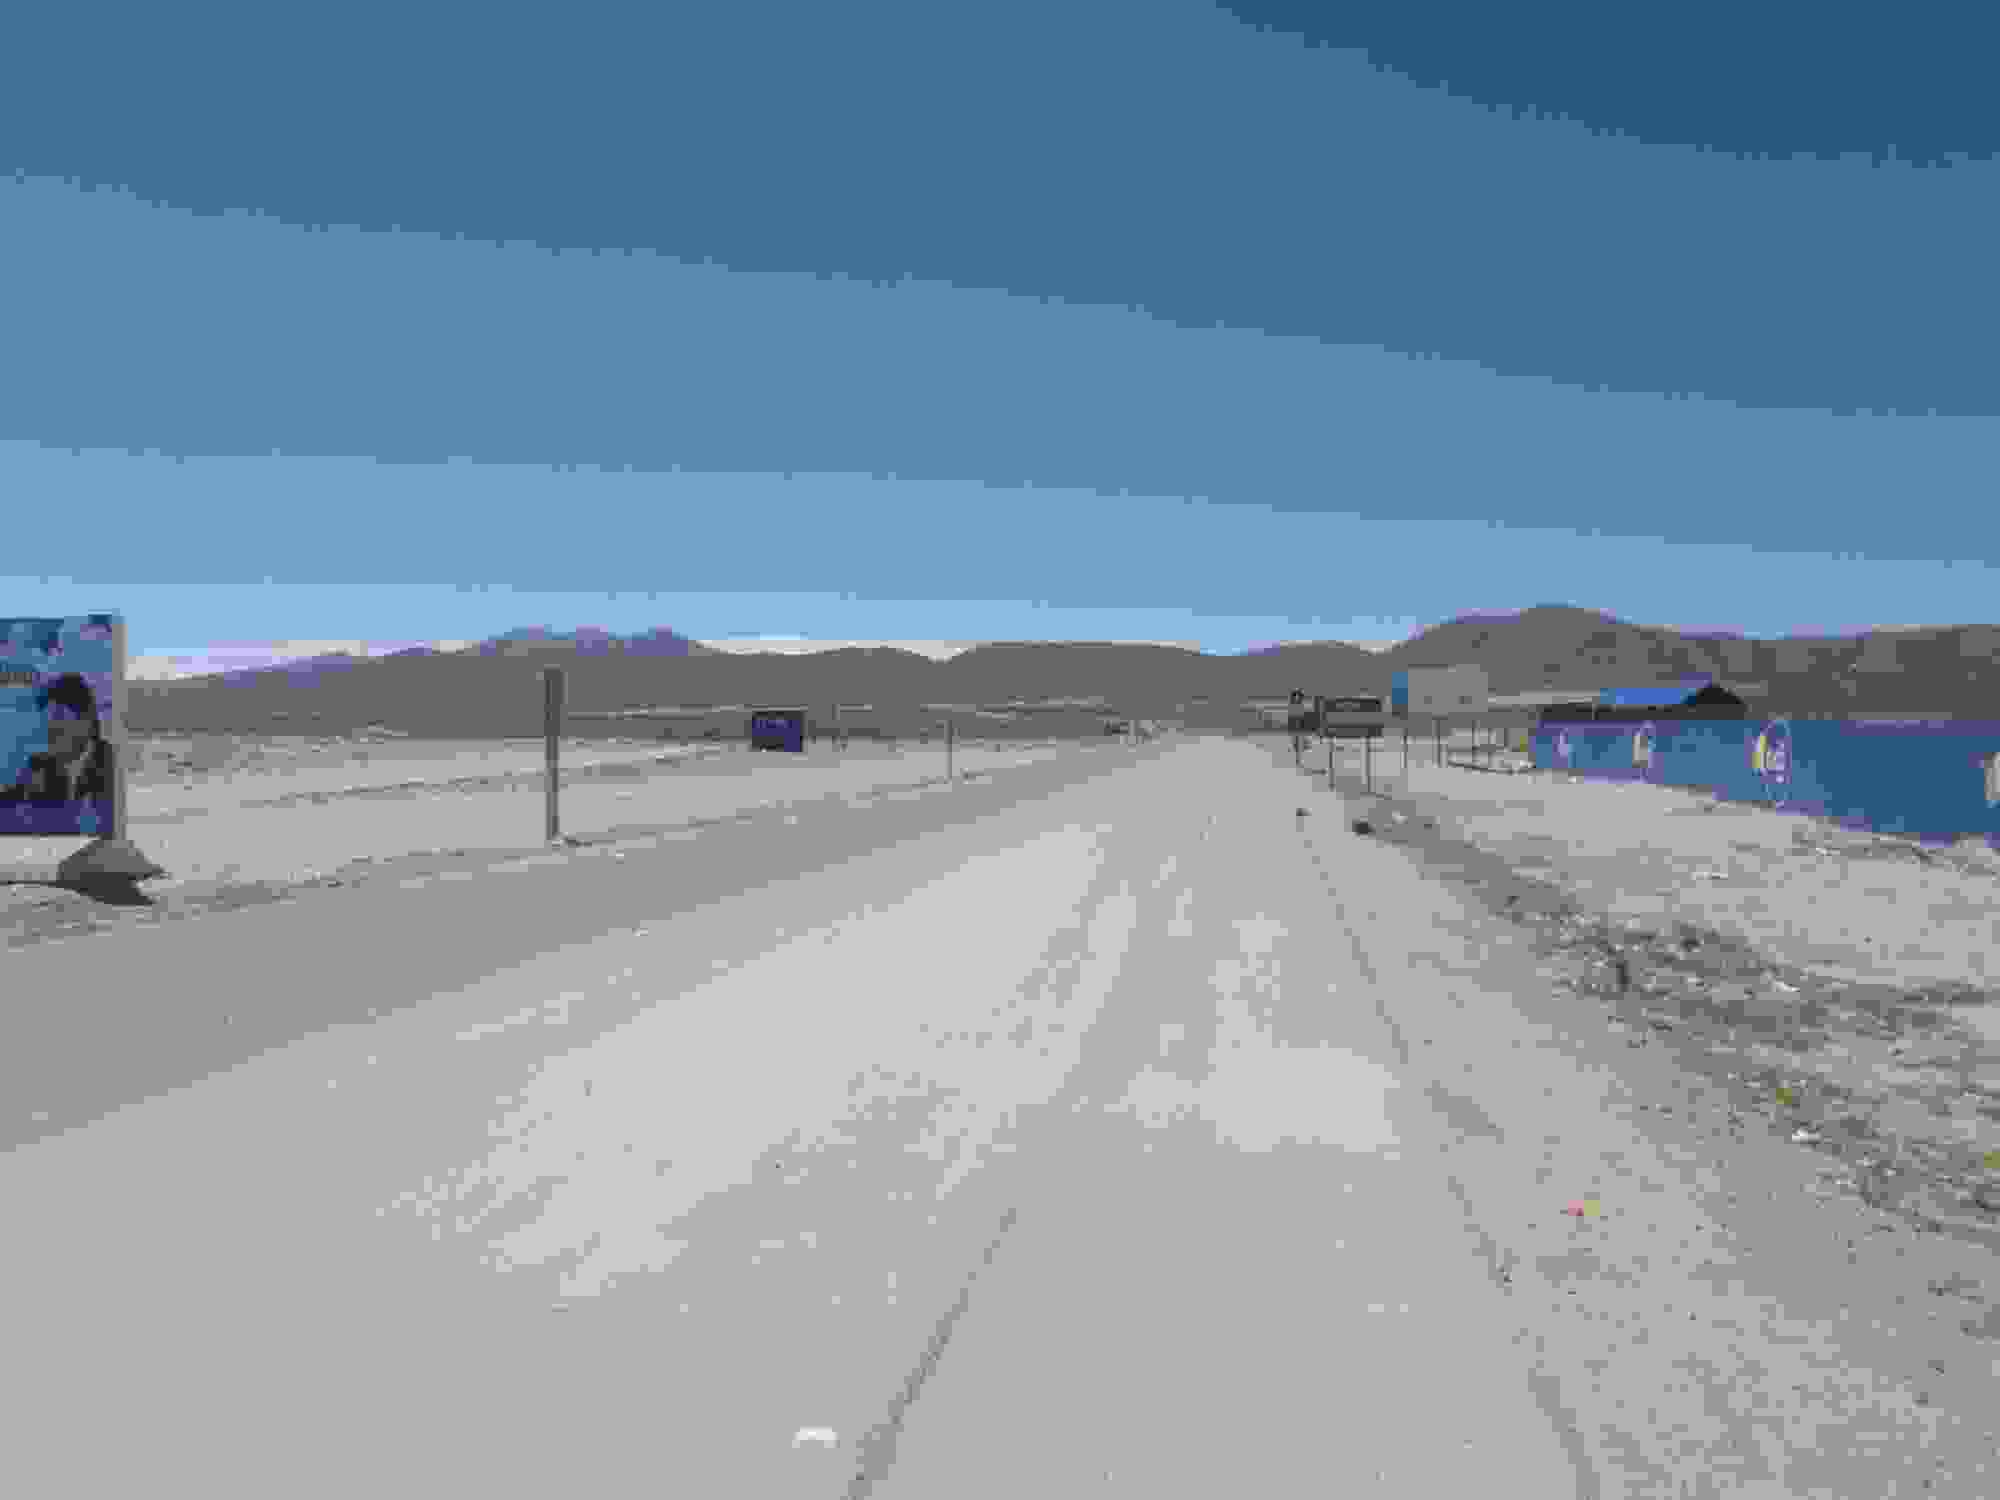
\includegraphics[width=\mywidth]{../wp-content/uploads/2015/04/wpid-wp-1428889869048.jpg} \end{center}
\vspace{-\topsep}

\pagebreak
 200km avec beaucoup de dénivelé, les paysages sont variés. 
\begin{center} 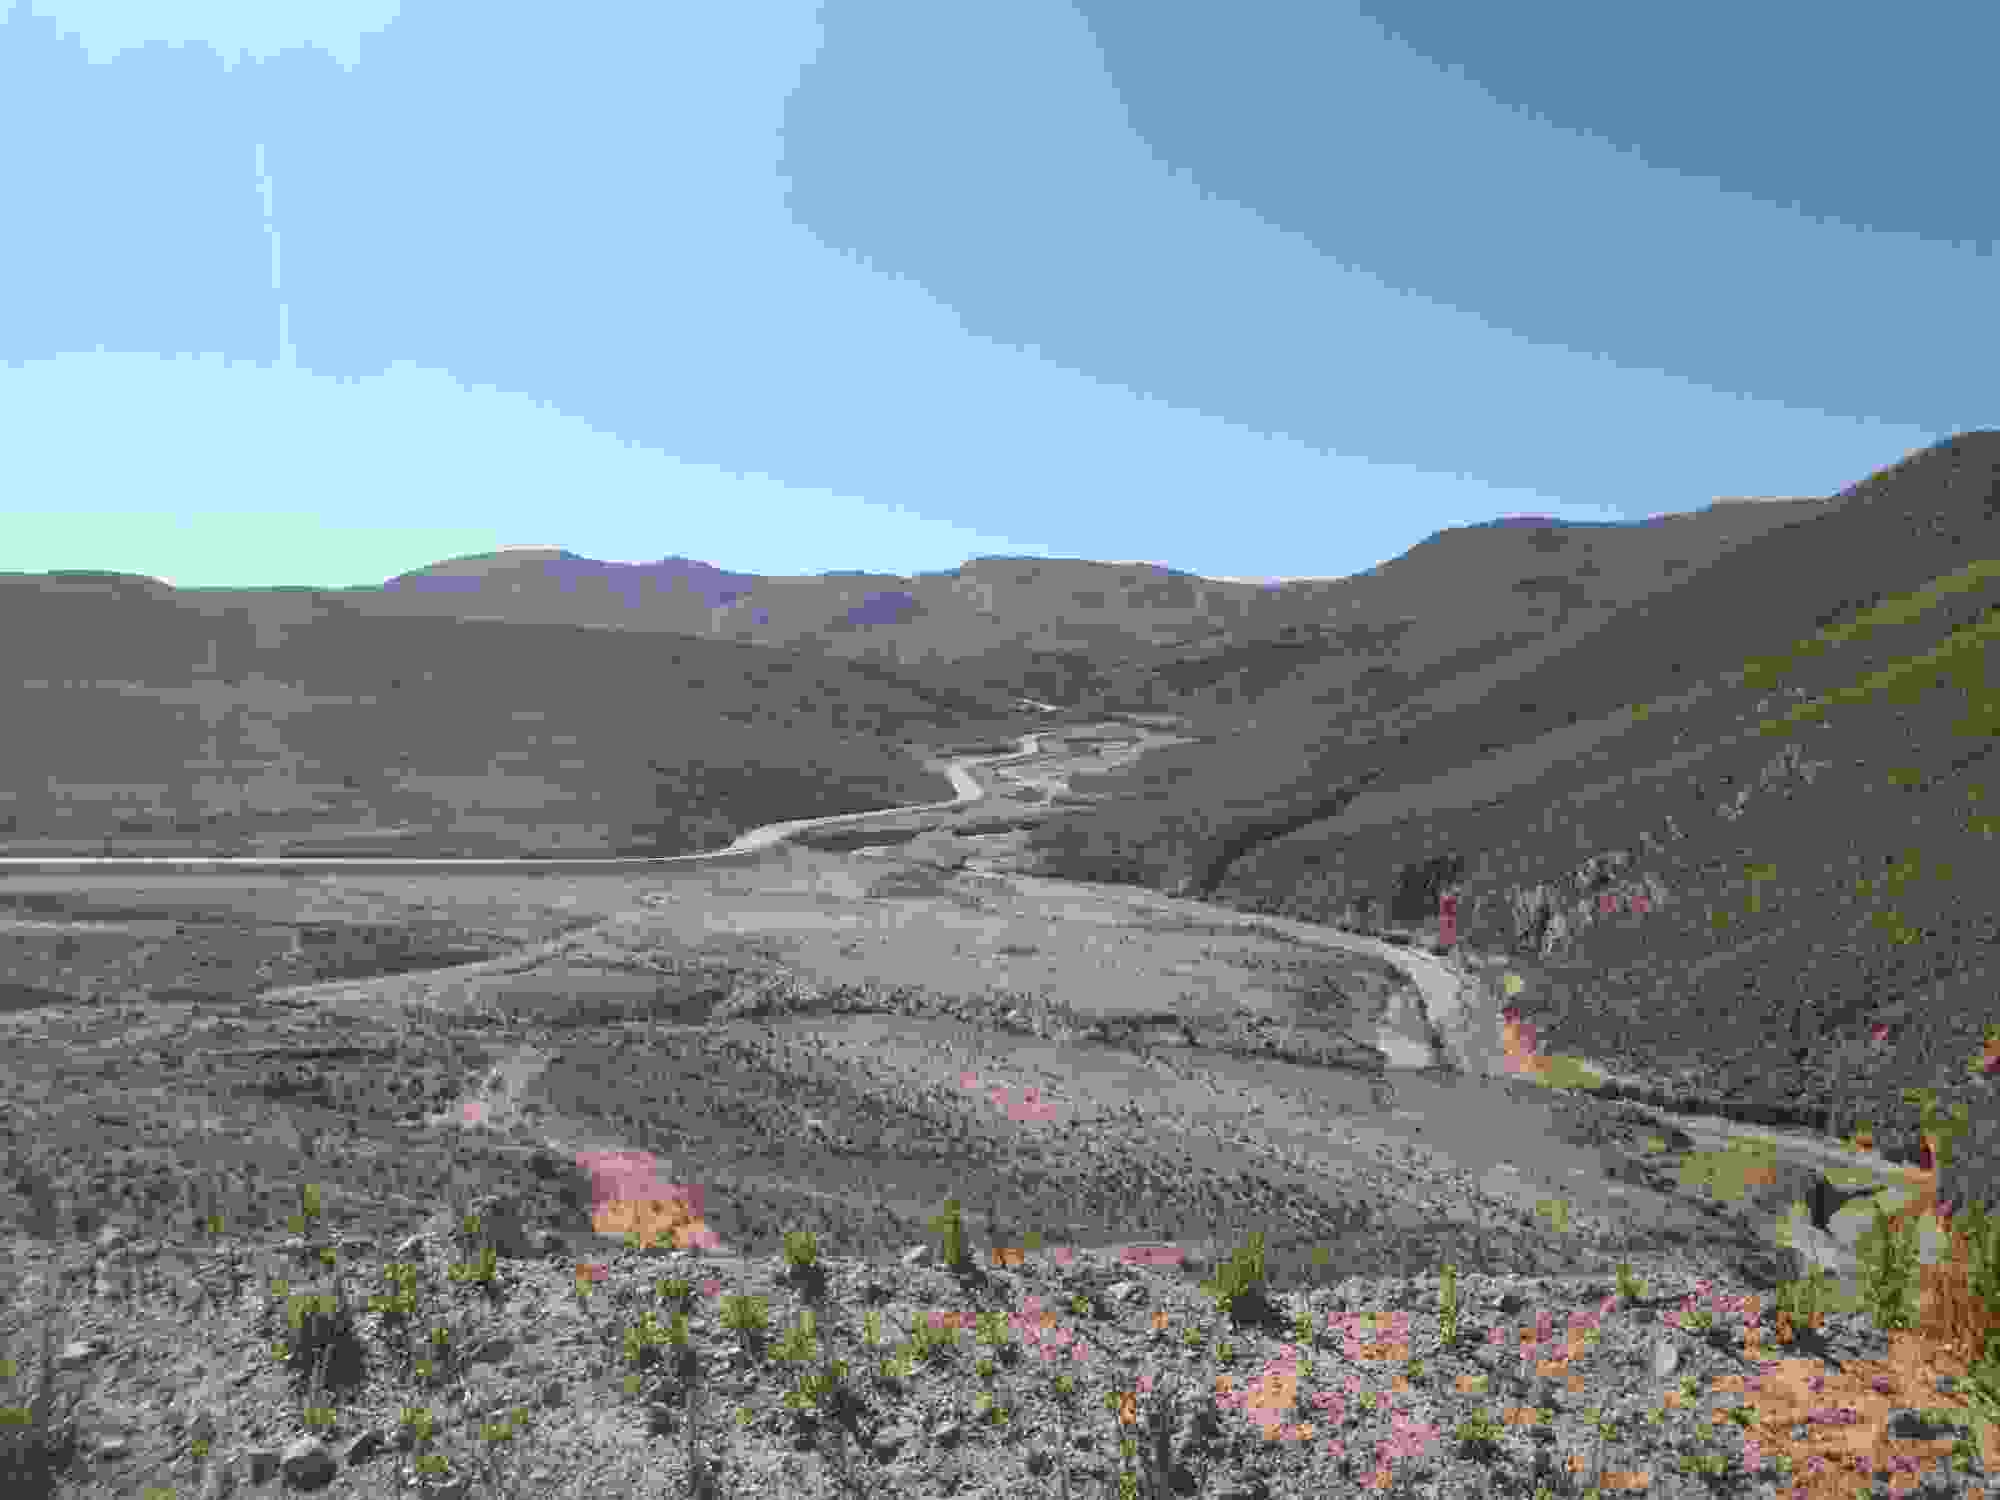
\includegraphics[width=\mywidth]{../wp-content/uploads/2015/04/wpid-wp-1428890082796.jpg} \end{center}
\begin{center} 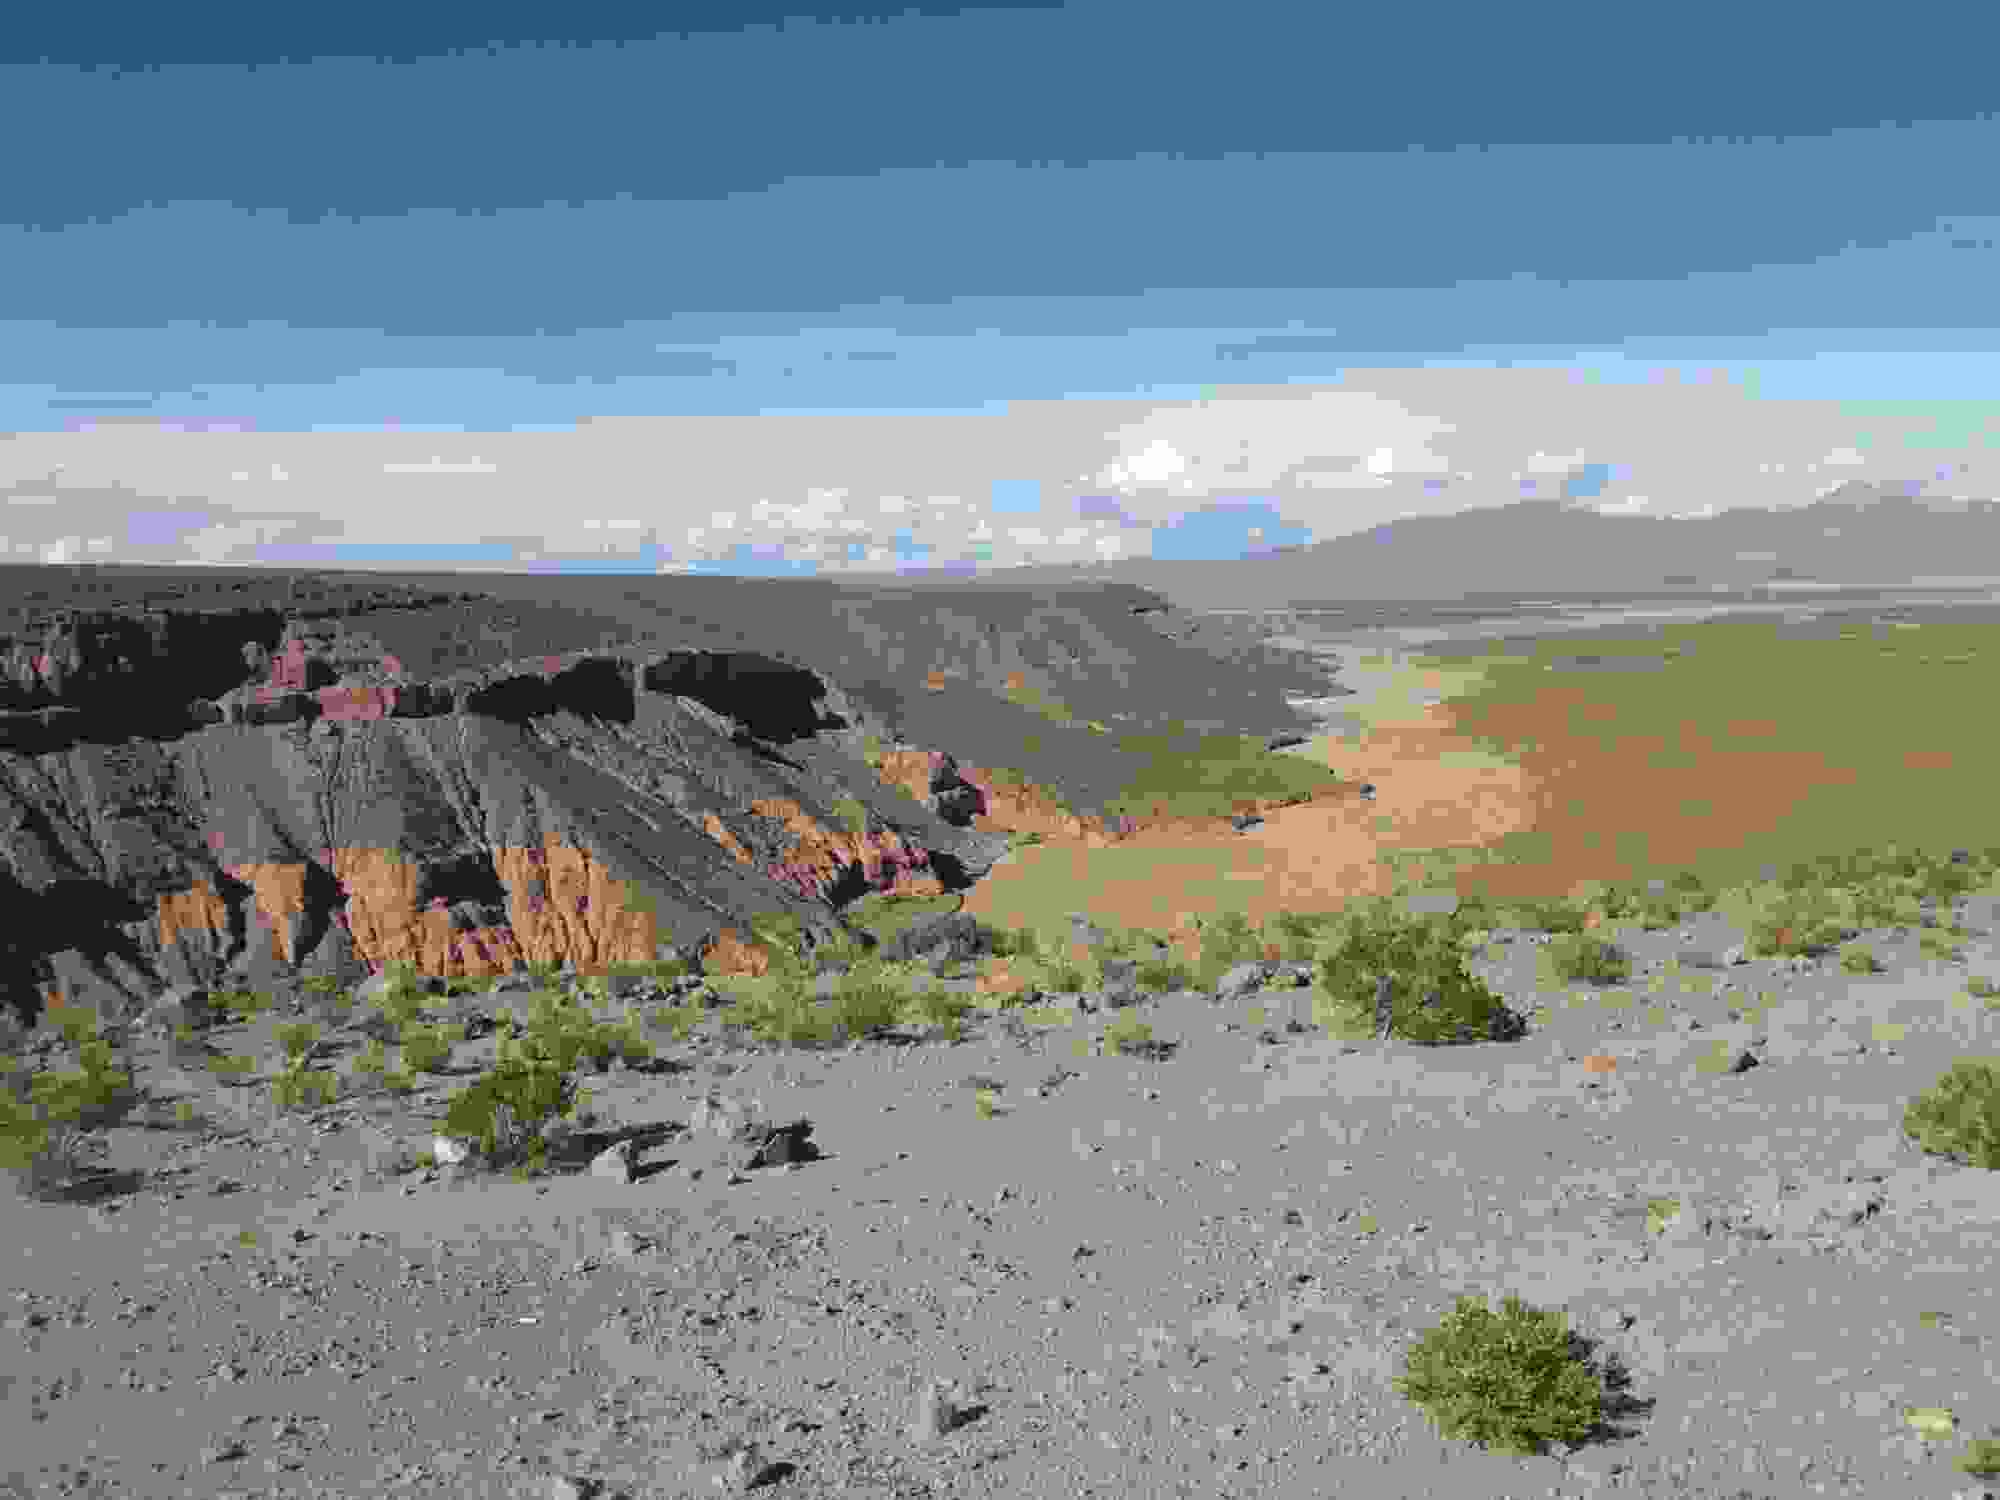
\includegraphics[width=\mywidth]{../wp-content/uploads/2015/04/wpid-wp-1428890125837.jpg} \end{center}
\begin{center} 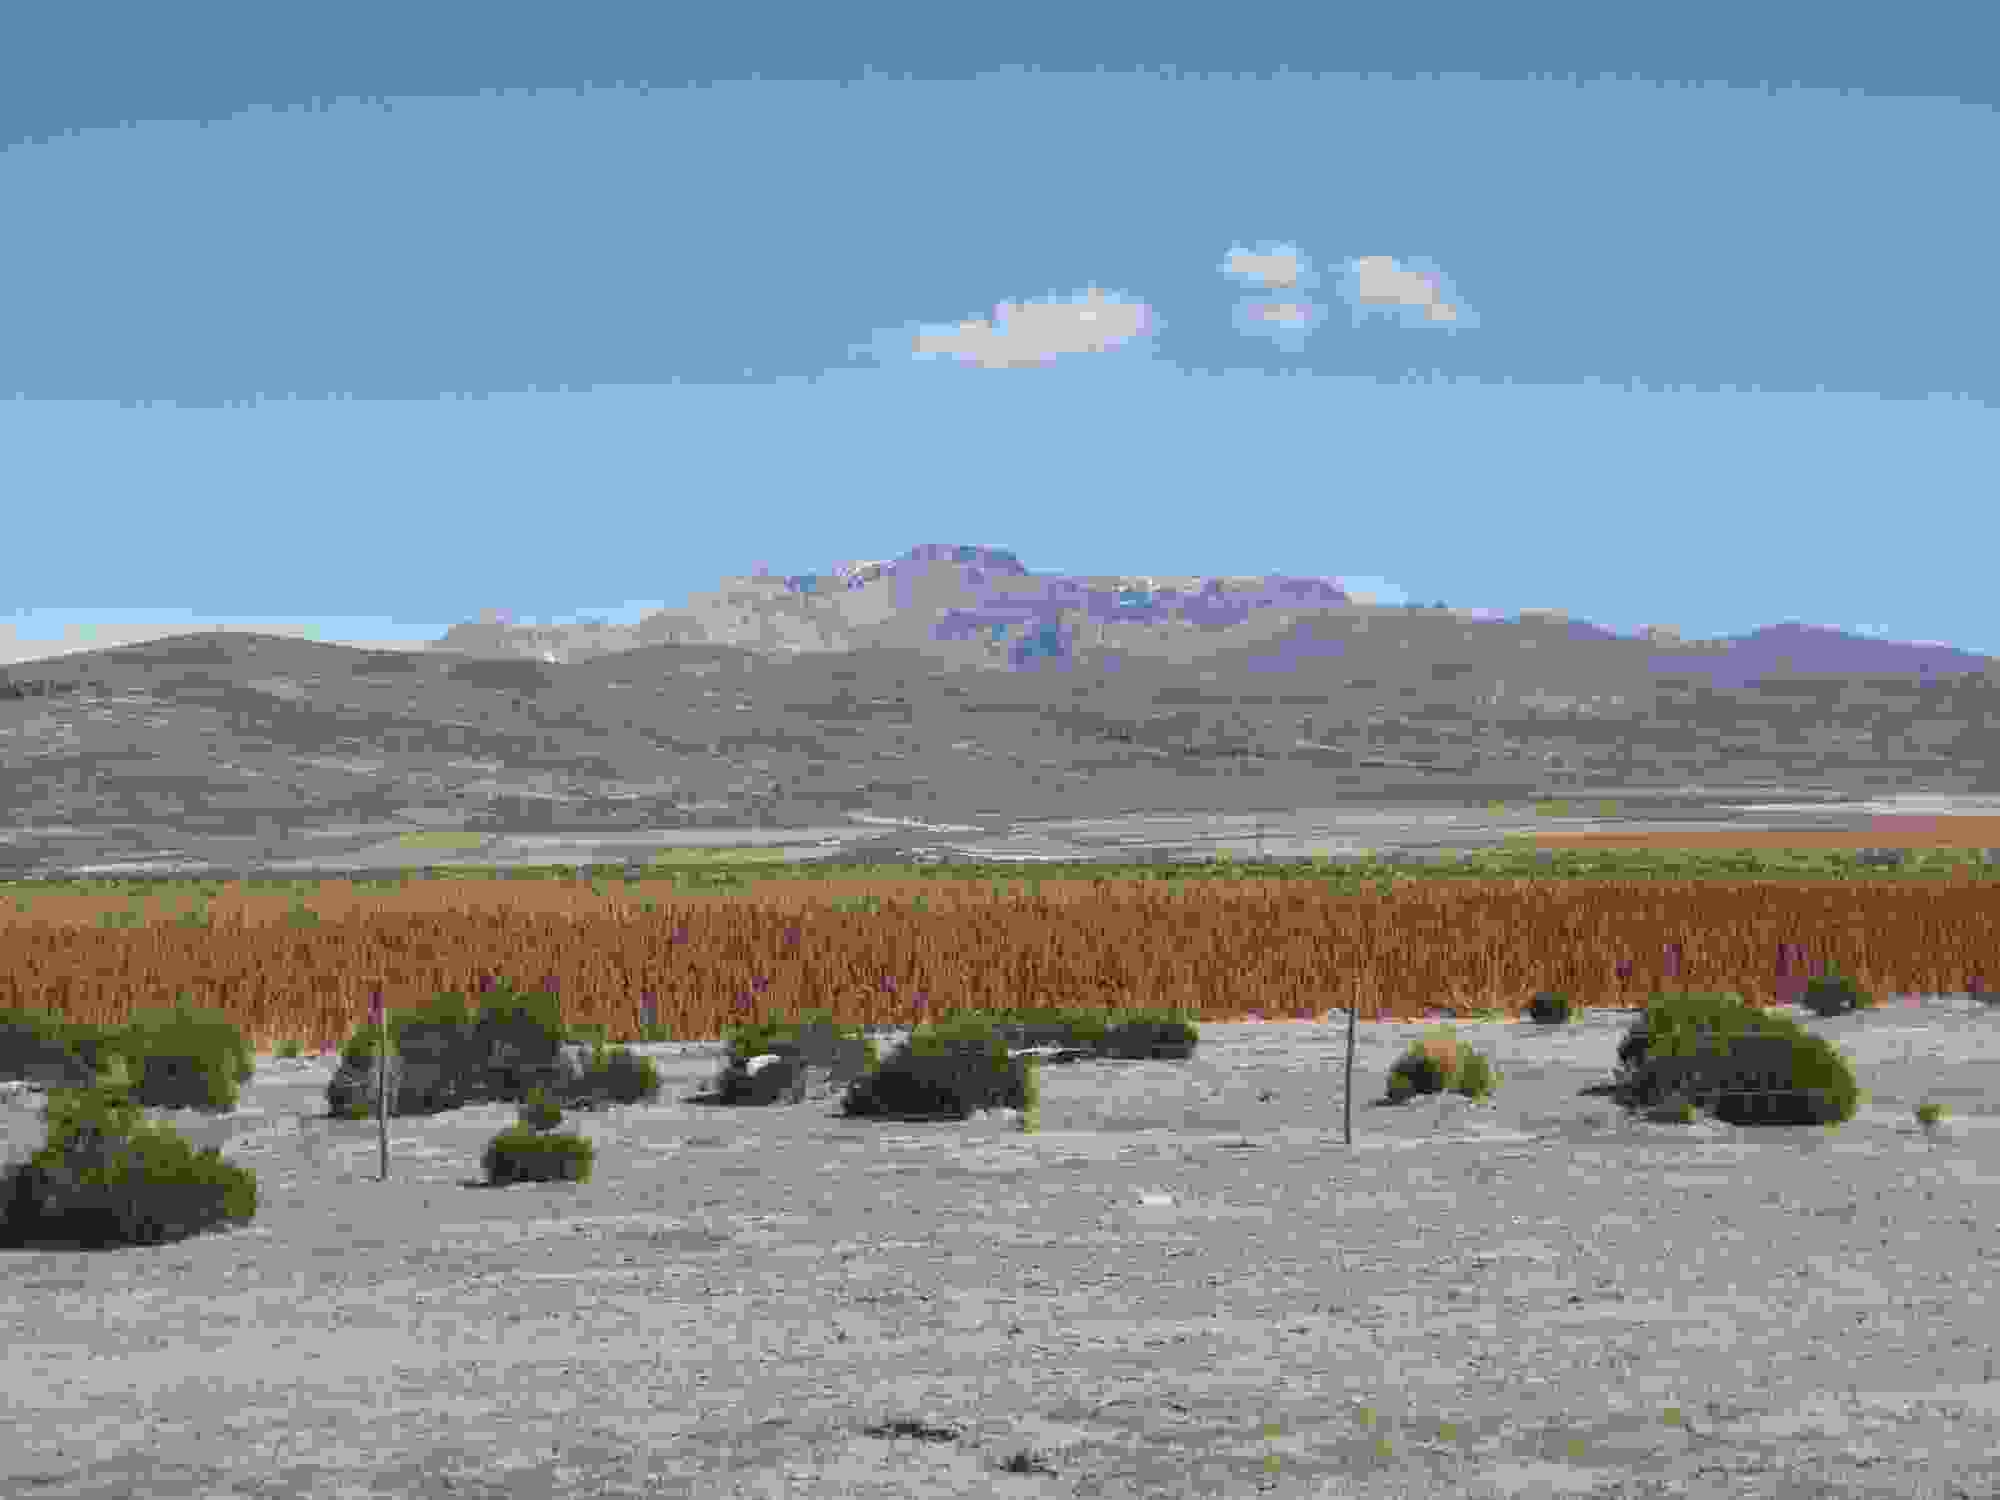
\includegraphics[width=\mywidth]{../wp-content/uploads/2015/04/wpid-wp-1428890169790.jpg} \end{center}
\begin{center} 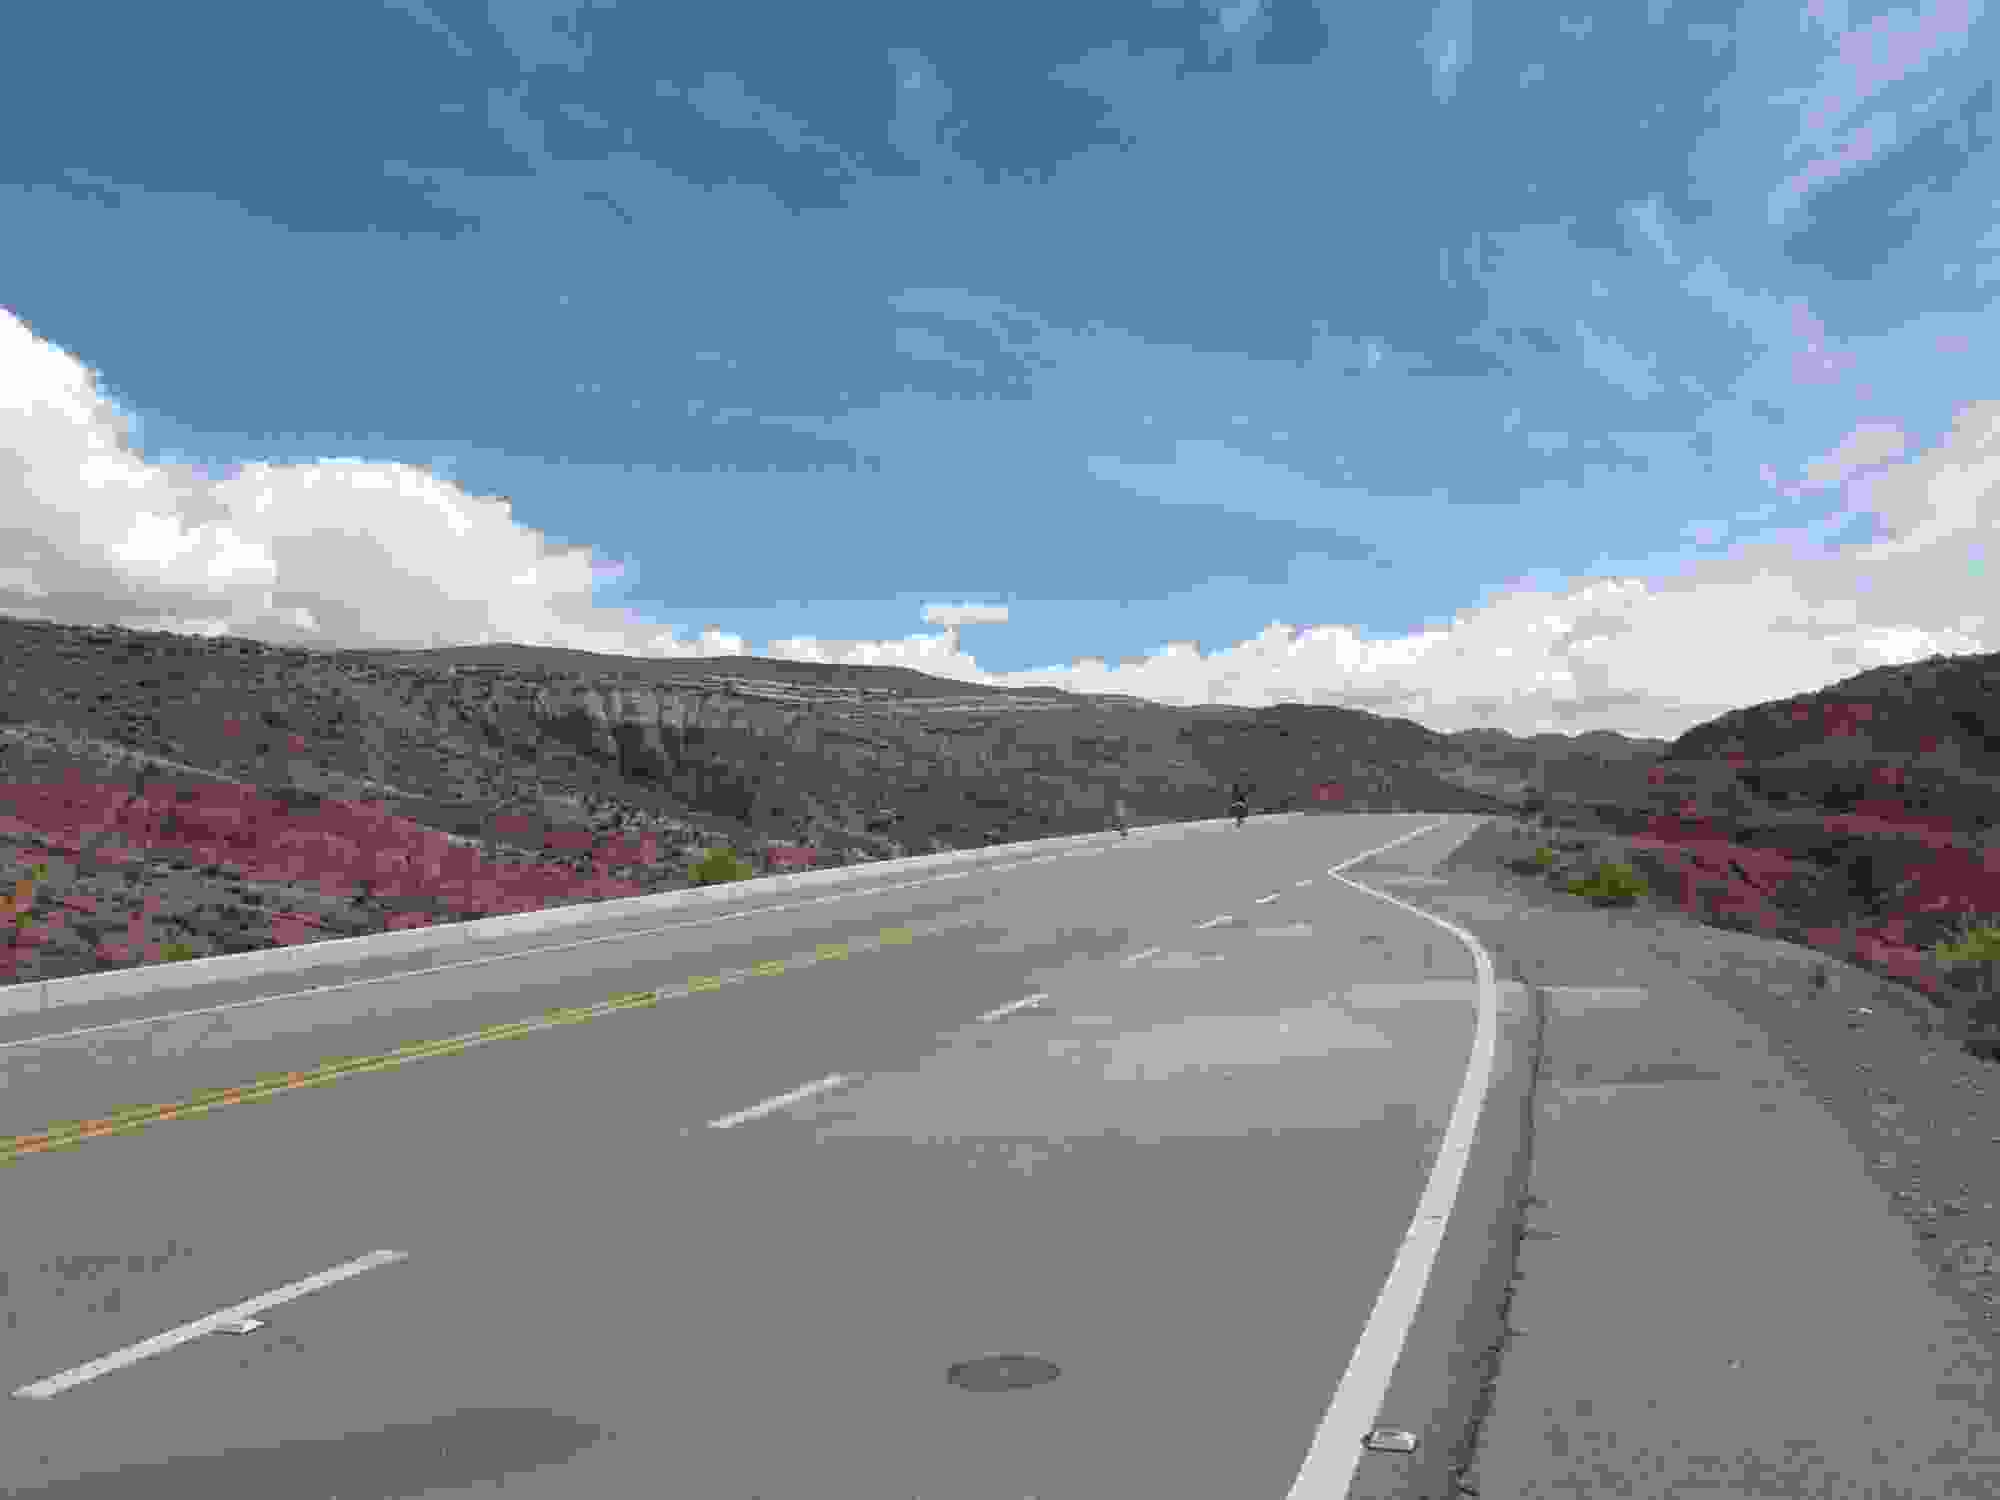
\includegraphics[width=\mywidth]{../wp-content/uploads/2015/04/wpid-wp-1428890252937.jpg} \end{center}
\begin{center} 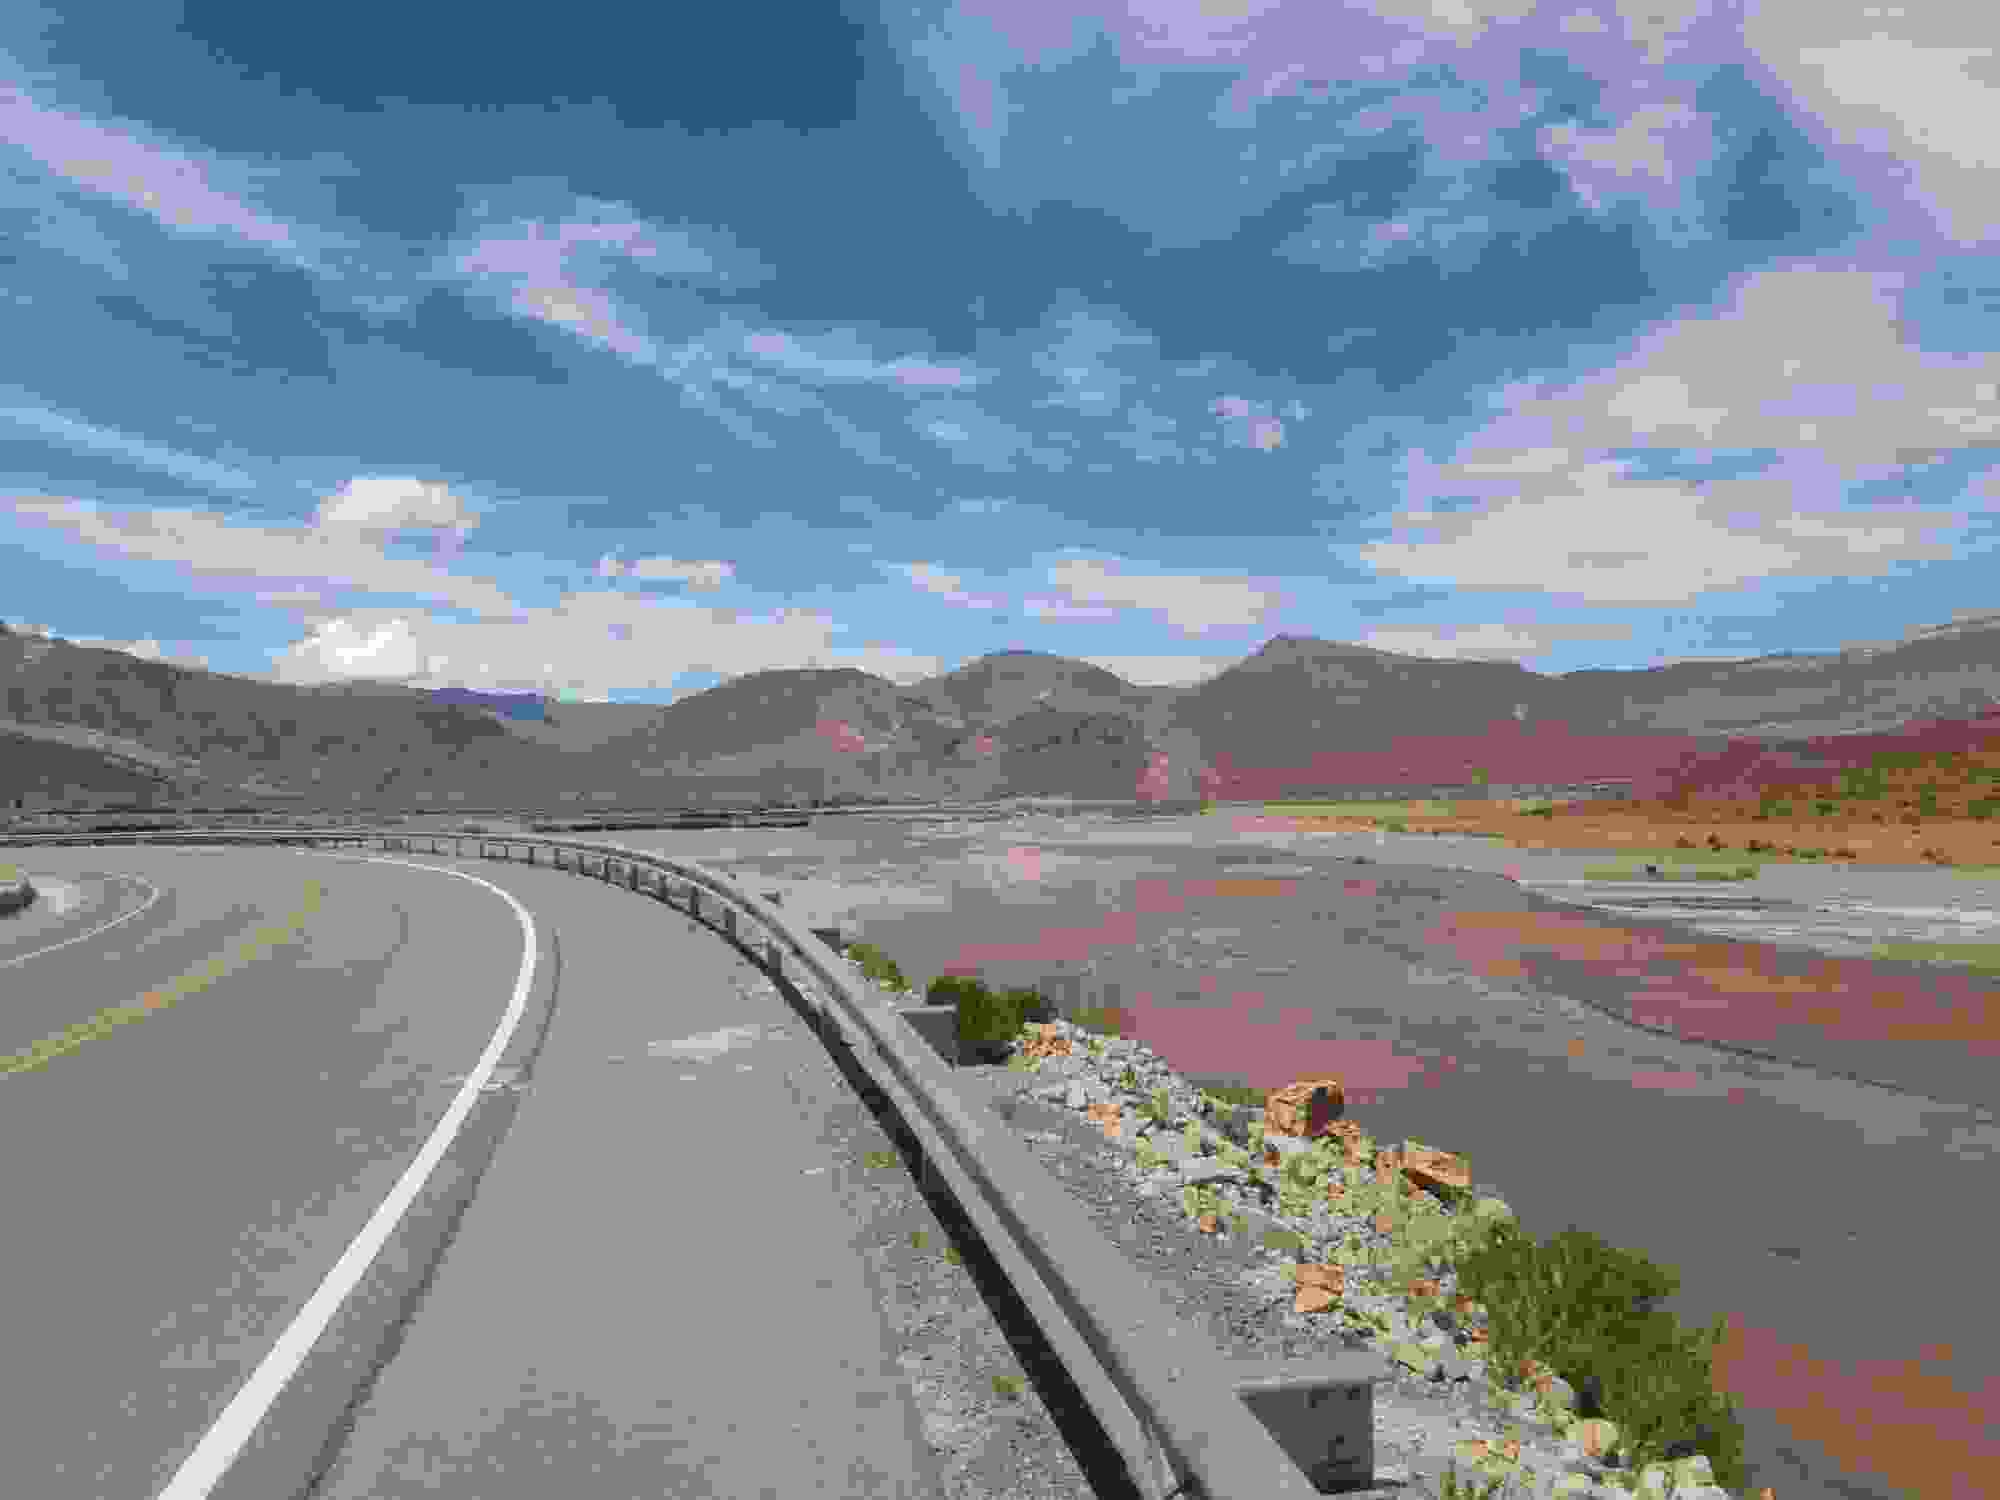
\includegraphics[width=\mywidth]{../wp-content/uploads/2015/04/wpid-wp-1428890285088.jpg} \end{center}

 On traverse quelques villages.
\begin{center} 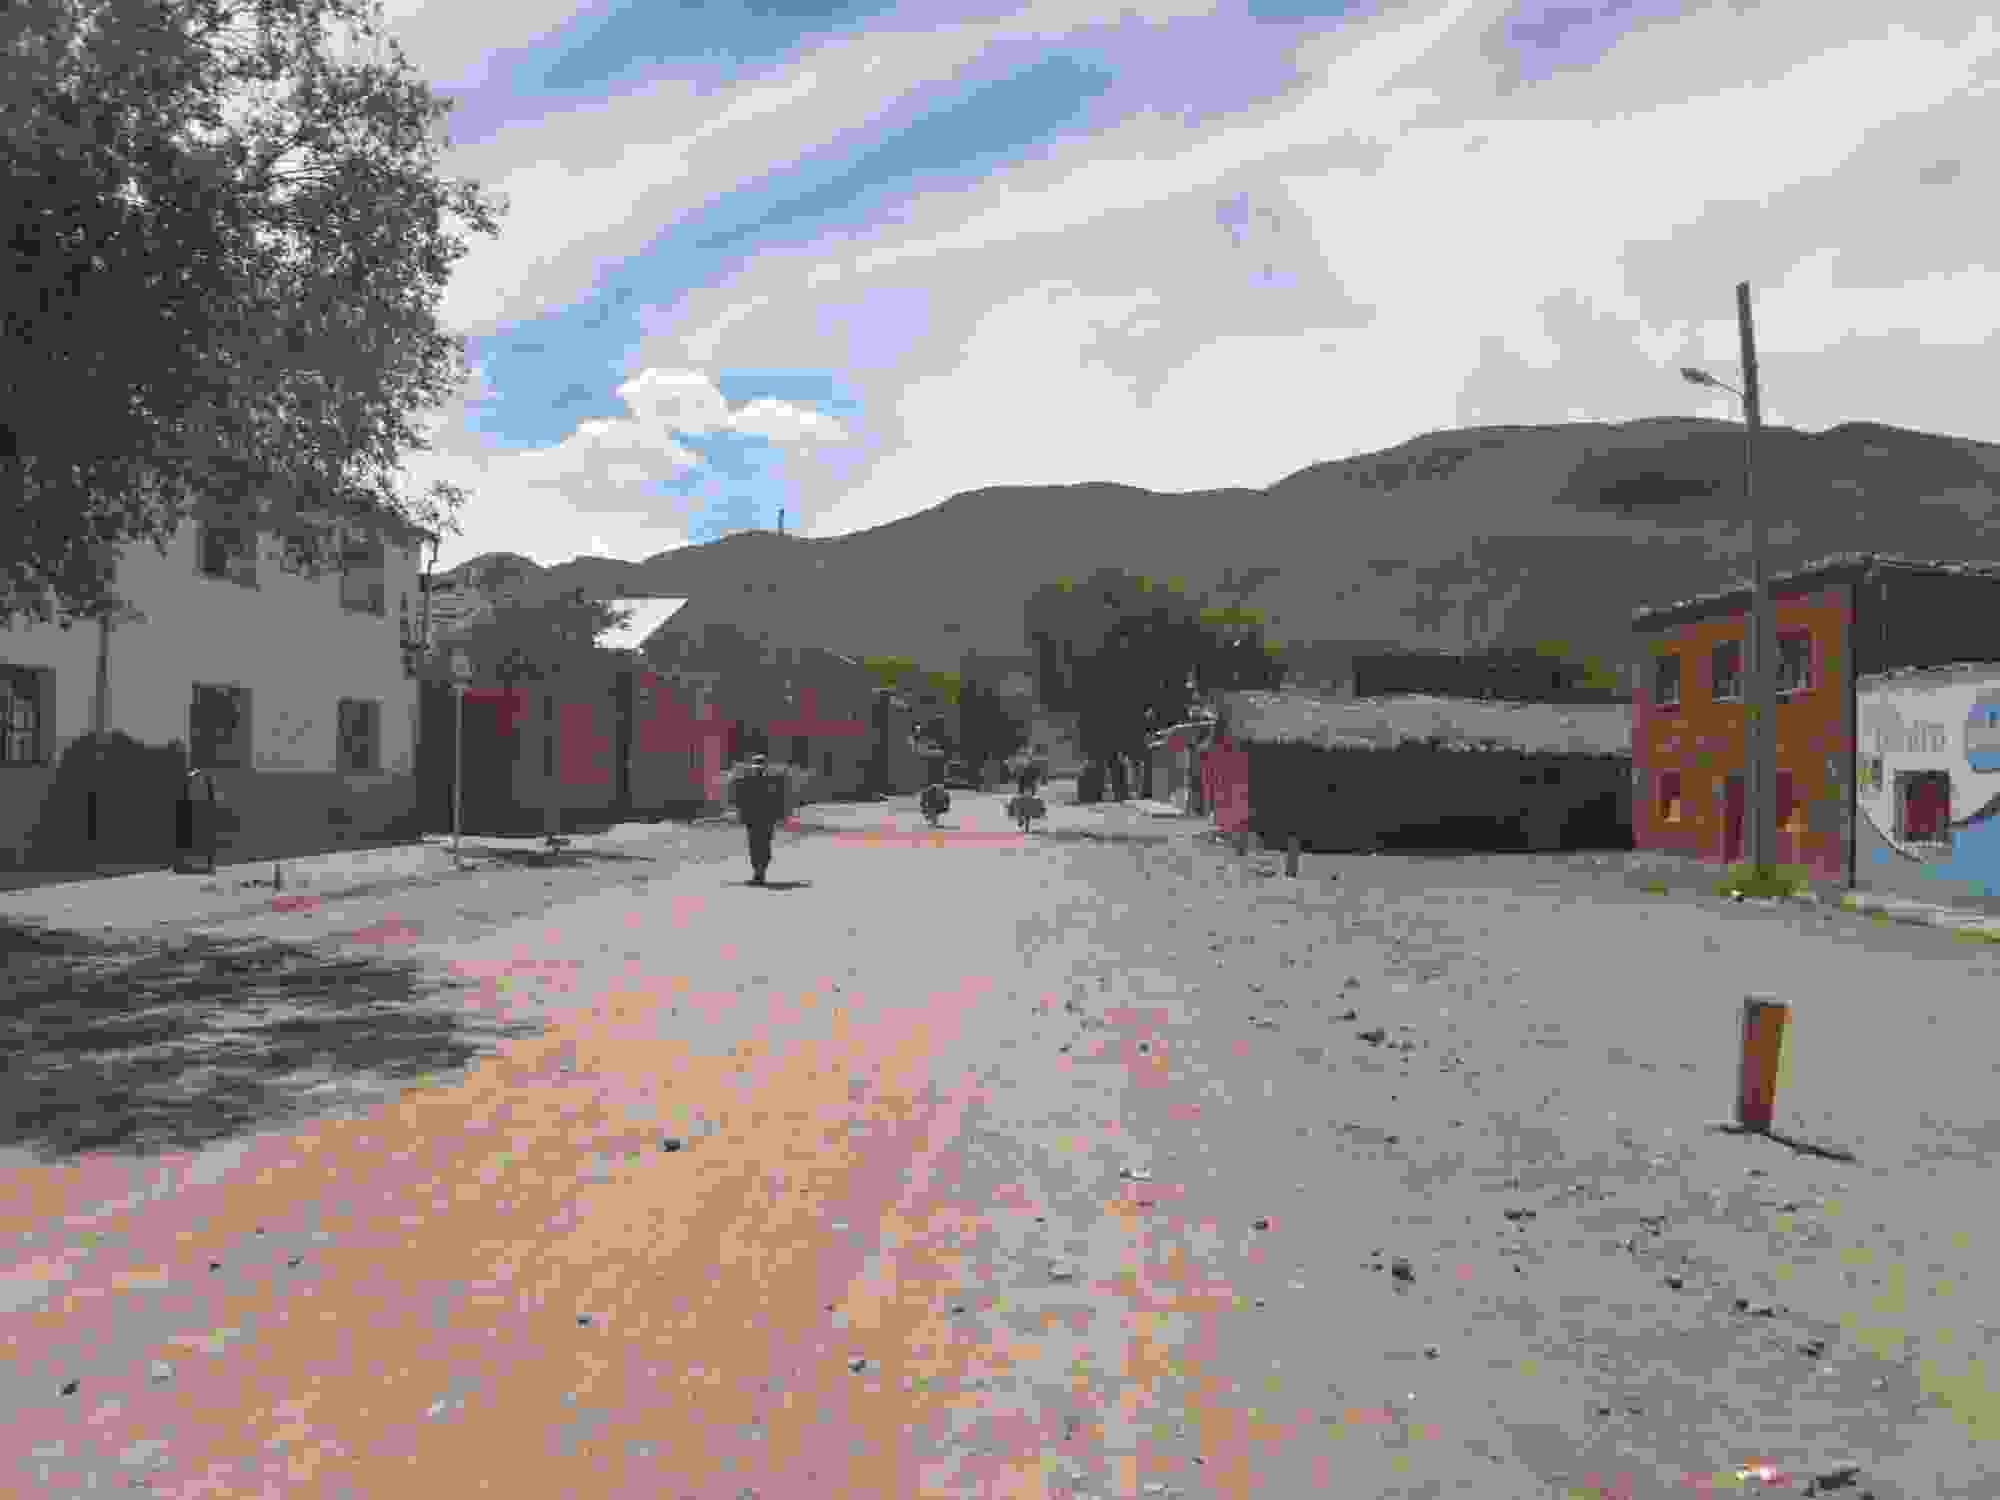
\includegraphics[width=\mywidth]{../wp-content/uploads/2015/04/wpid-wp-1428890373922.jpg} \end{center}
\begin{center} 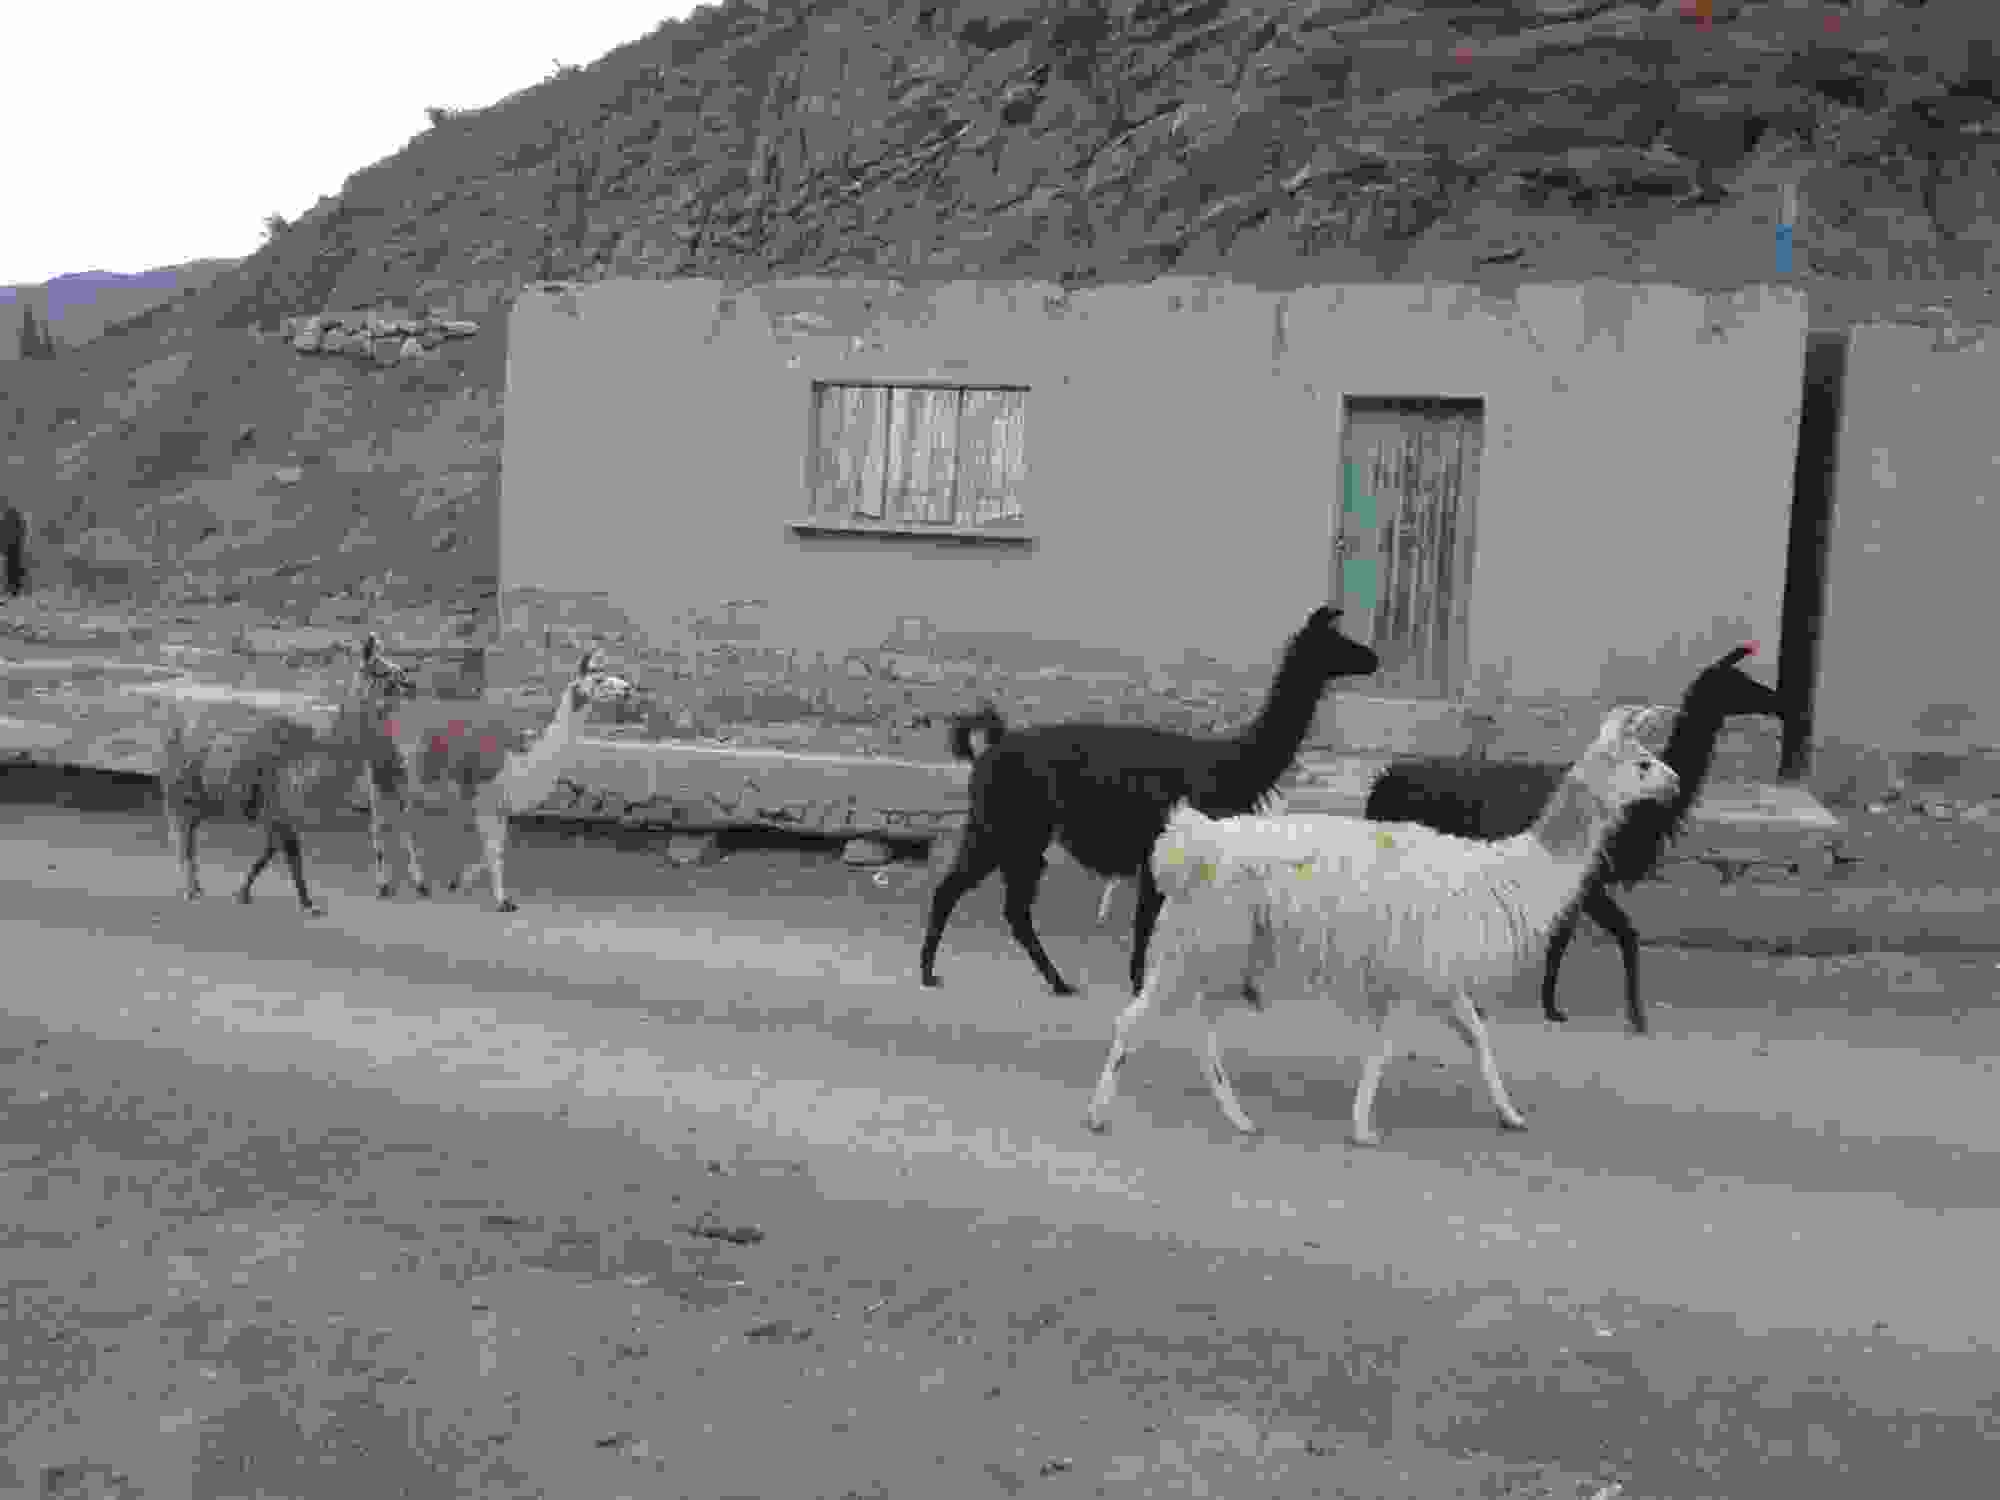
\includegraphics[width=\mywidth]{../wp-content/uploads/2015/04/wpid-wp-1428890480186.jpg} \end{center}

 Encore de beaux paysages. 
\begin{center} 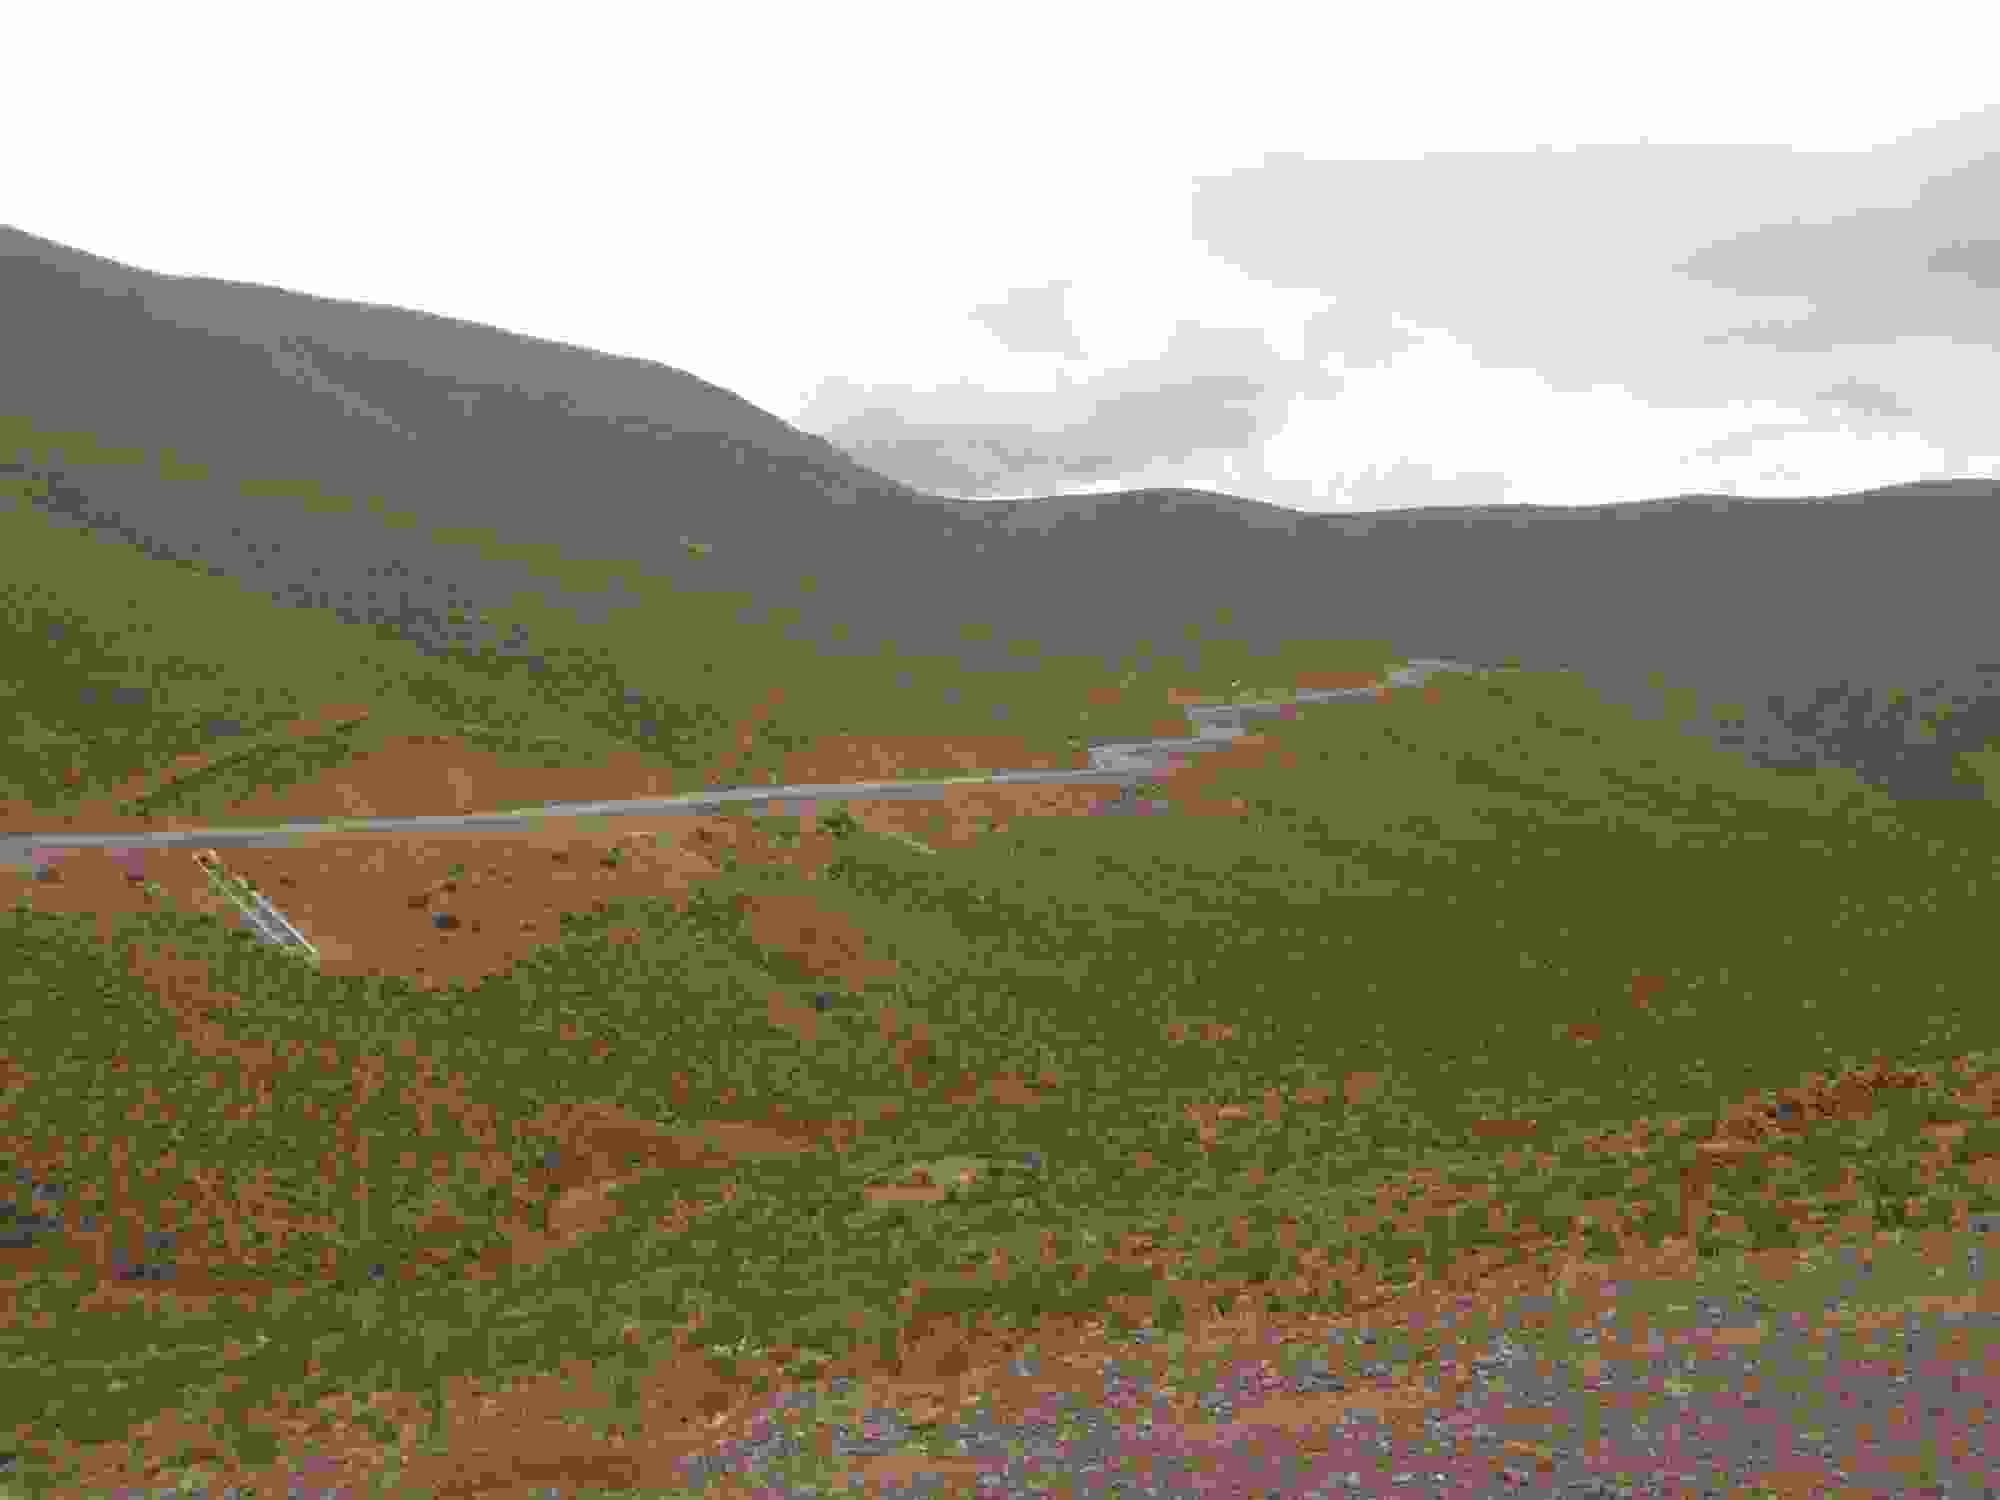
\includegraphics[width=\mywidth]{../wp-content/uploads/2015/04/wpid-wp-1428890534520.jpg} \end{center}
\begin{center} 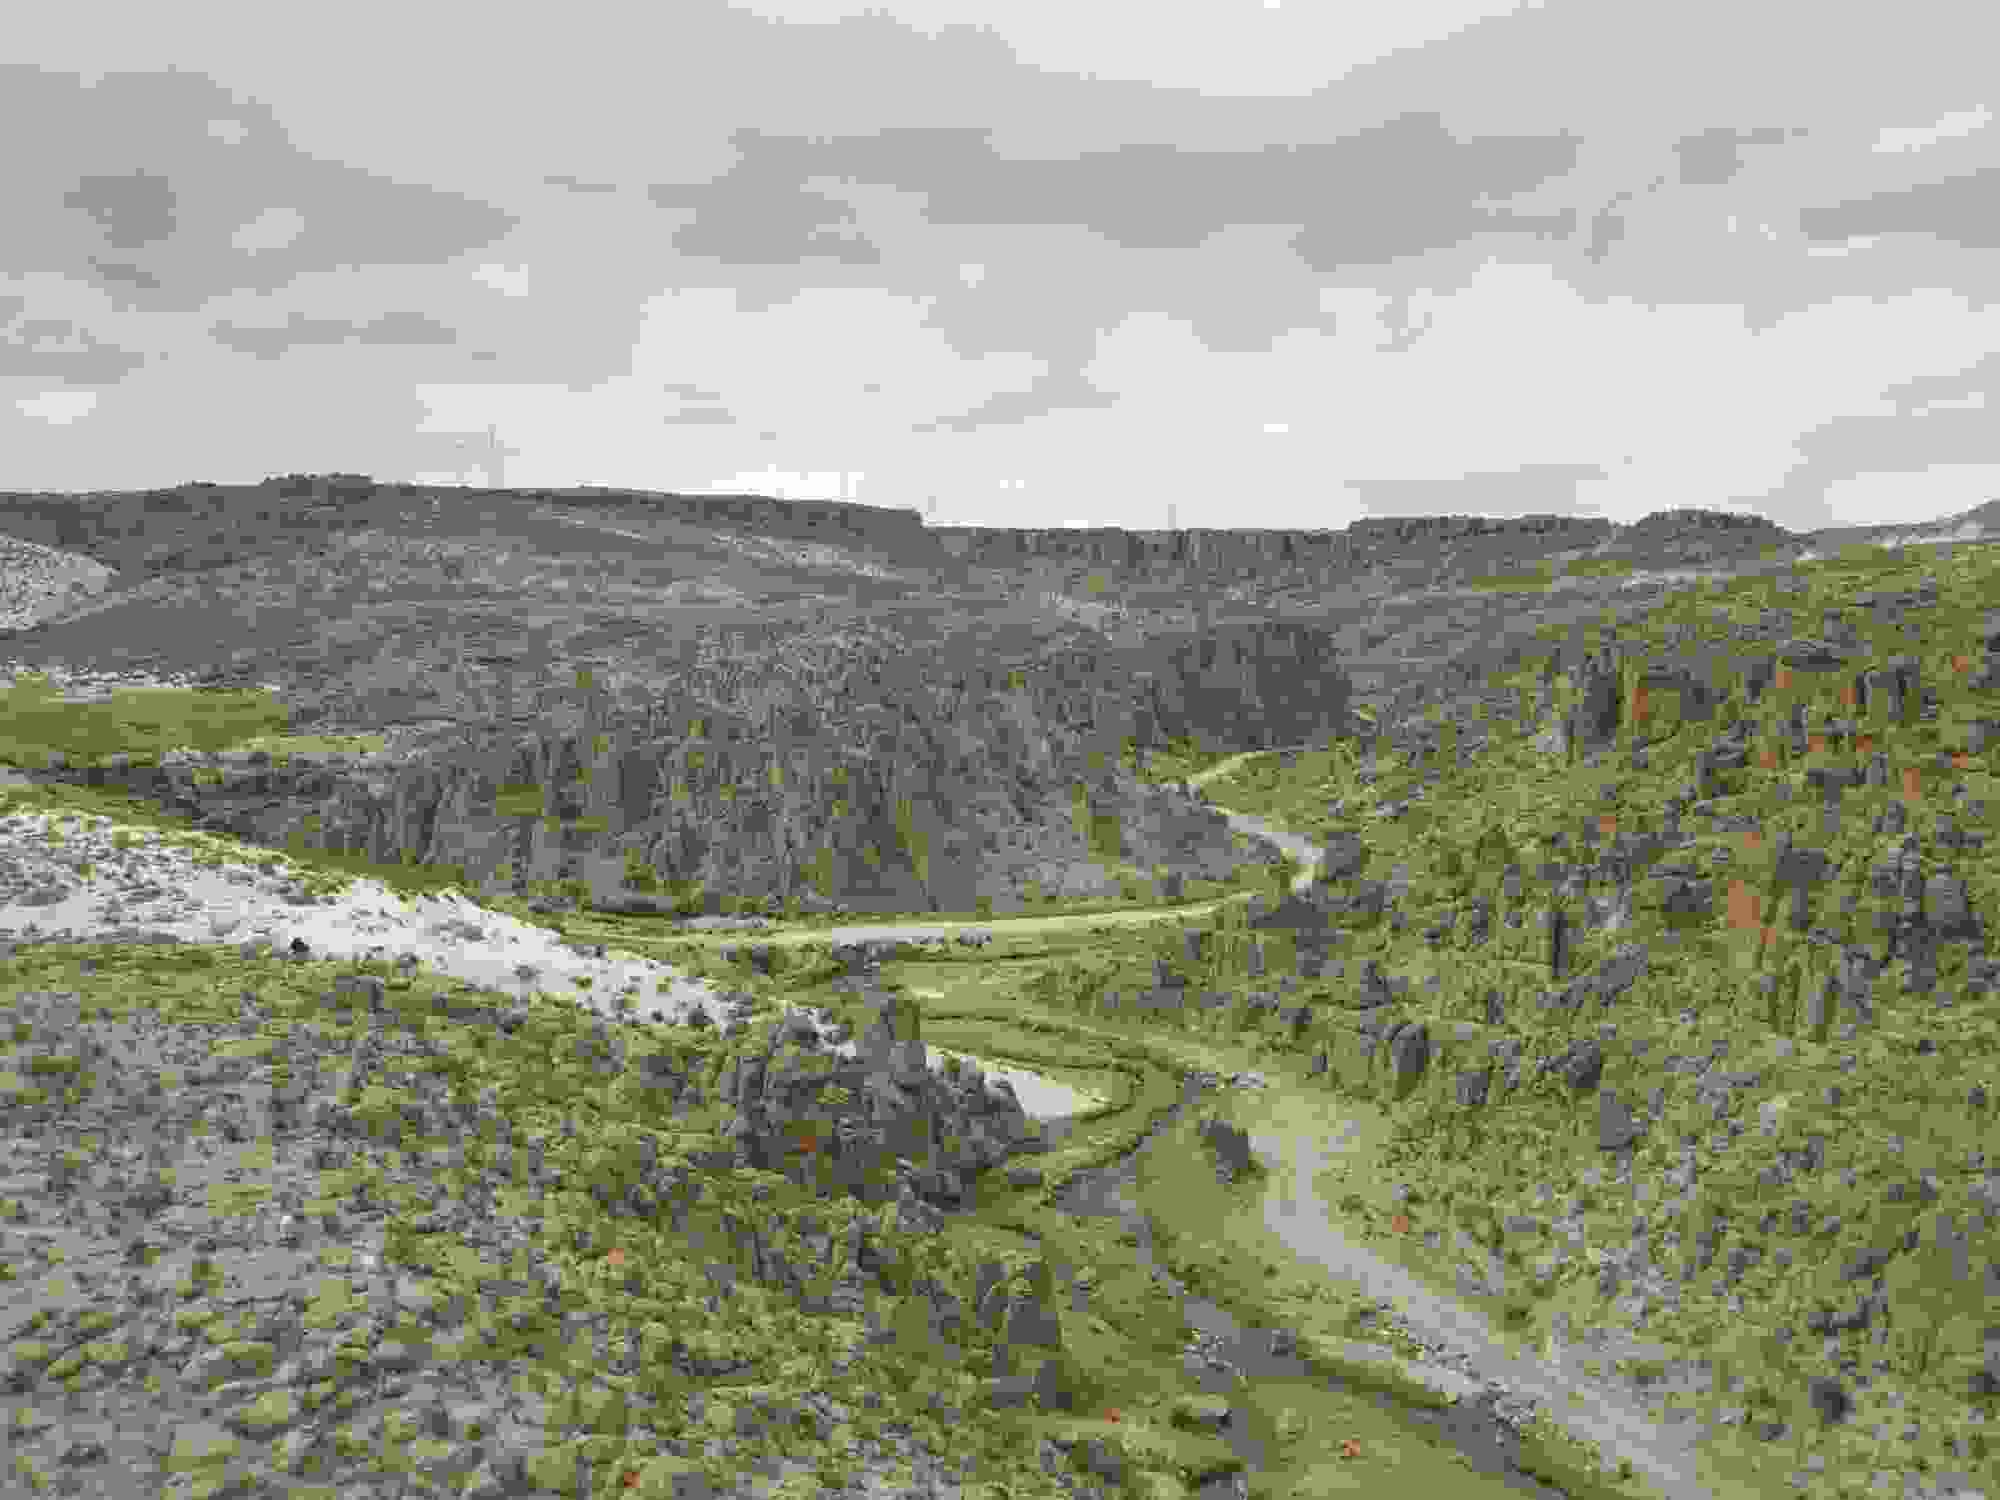
\includegraphics[width=\mywidth]{../wp-content/uploads/2015/04/wpid-wp-1428890635363.jpg} \end{center}

 Puis c'est l'arrivée à Potosí.
\begin{center} 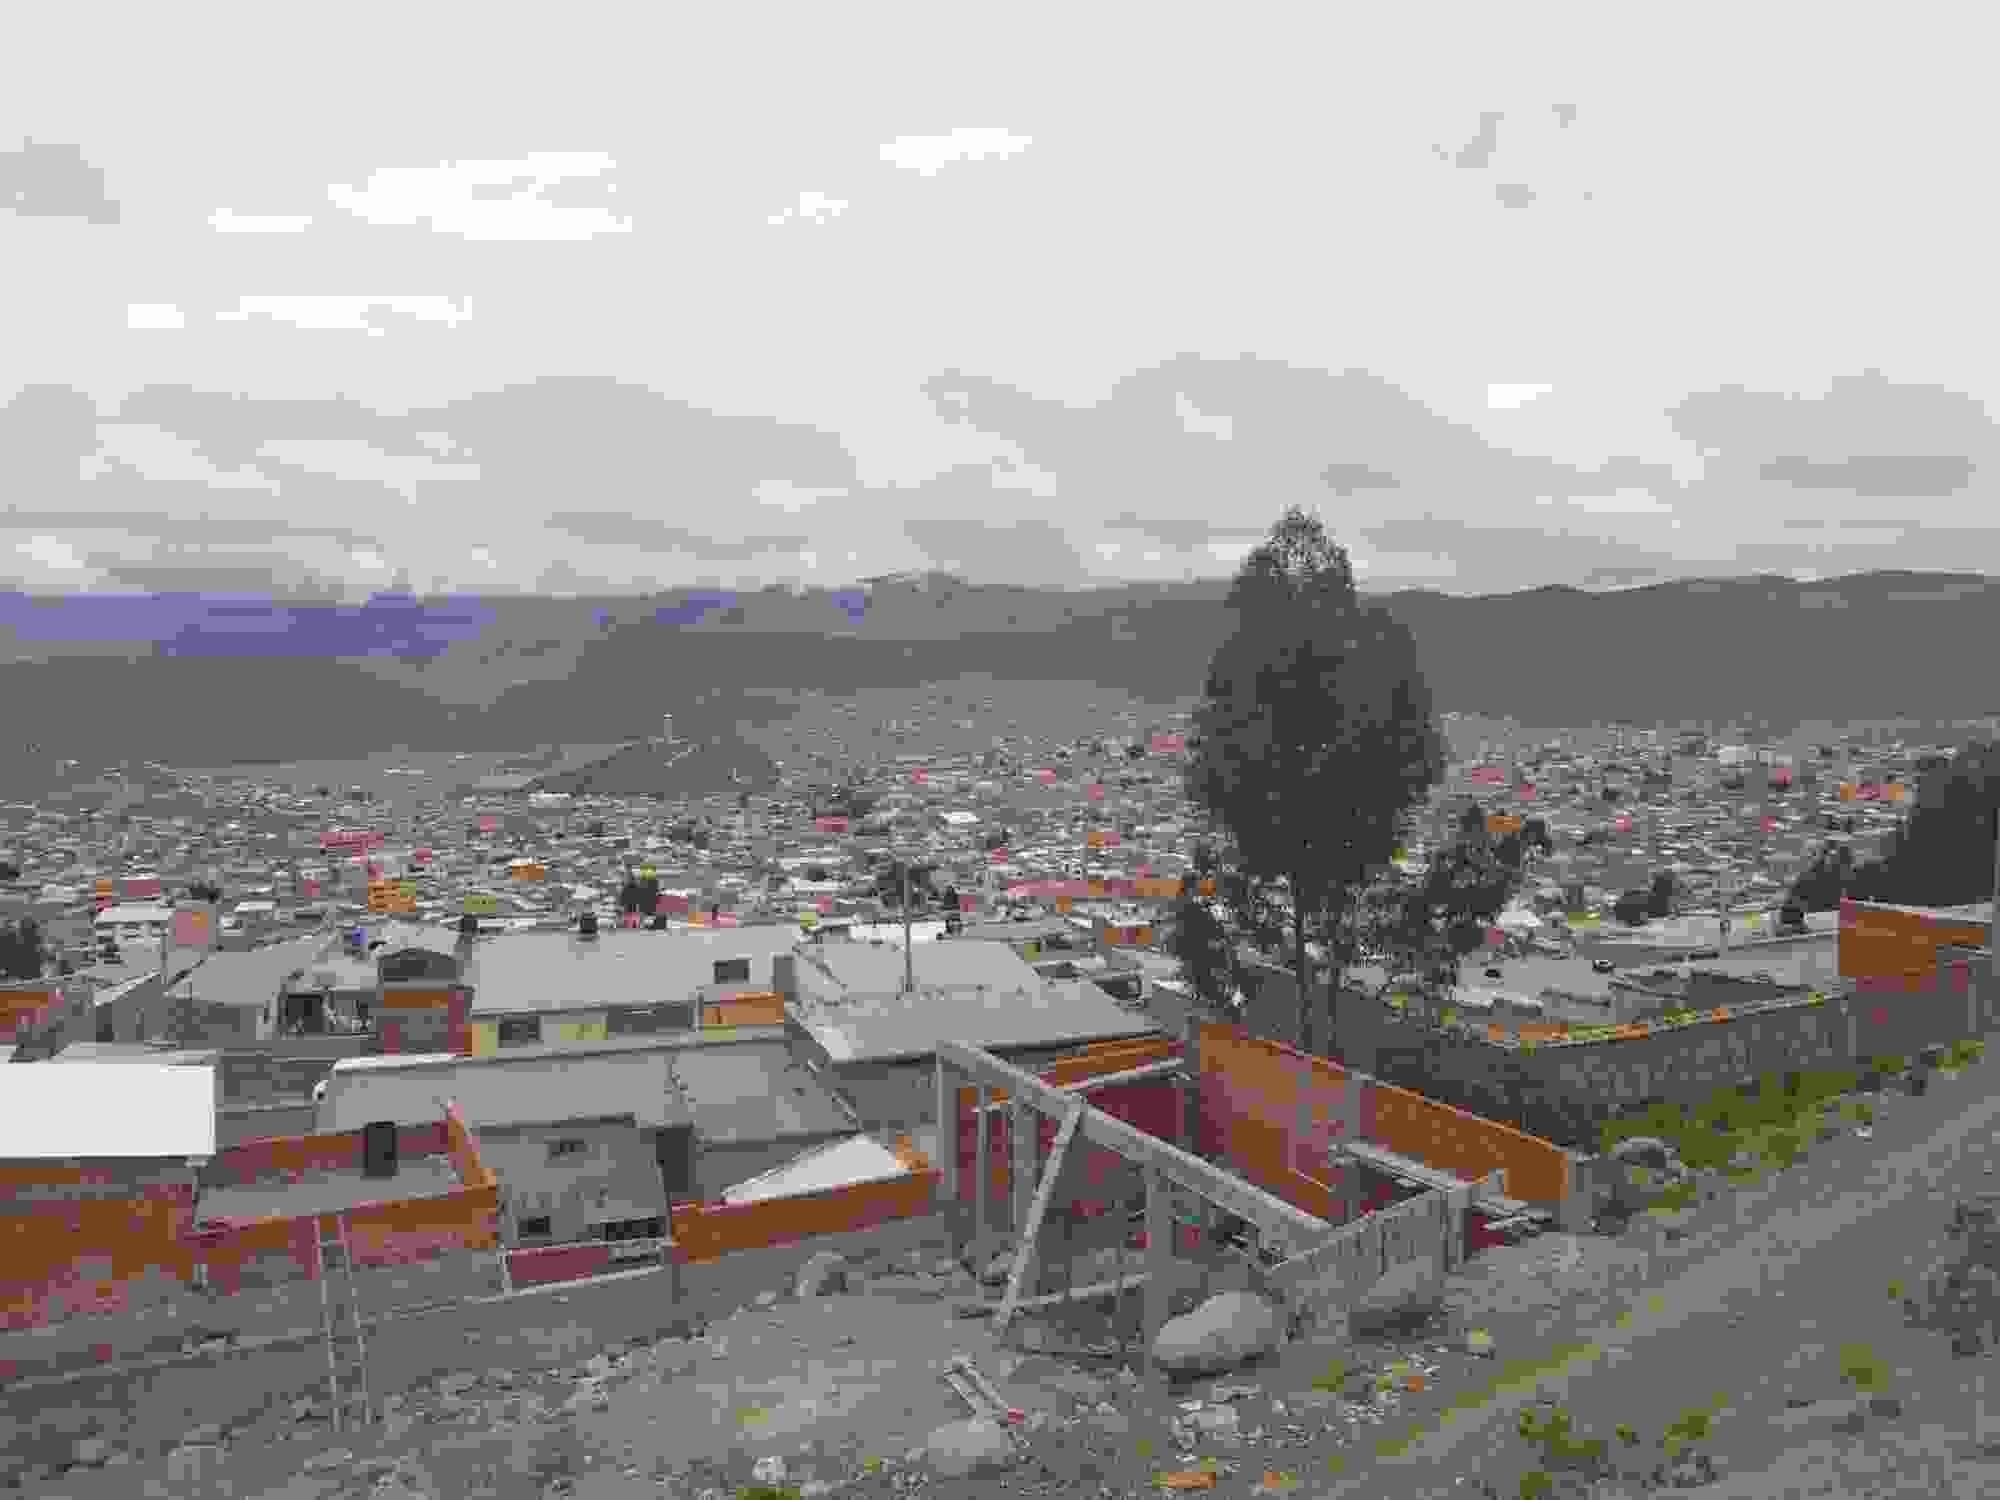
\includegraphics[width=\mywidth]{../wp-content/uploads/2015/04/wpid-wp-1428893483818.jpg} \end{center}
\vspace{-\topsep}

\pagebreak
 Un lac de couleur bizarre en contrebas de la ville : en fait ce sont les déchets des usines de traitement des minerais.
\begin{center} 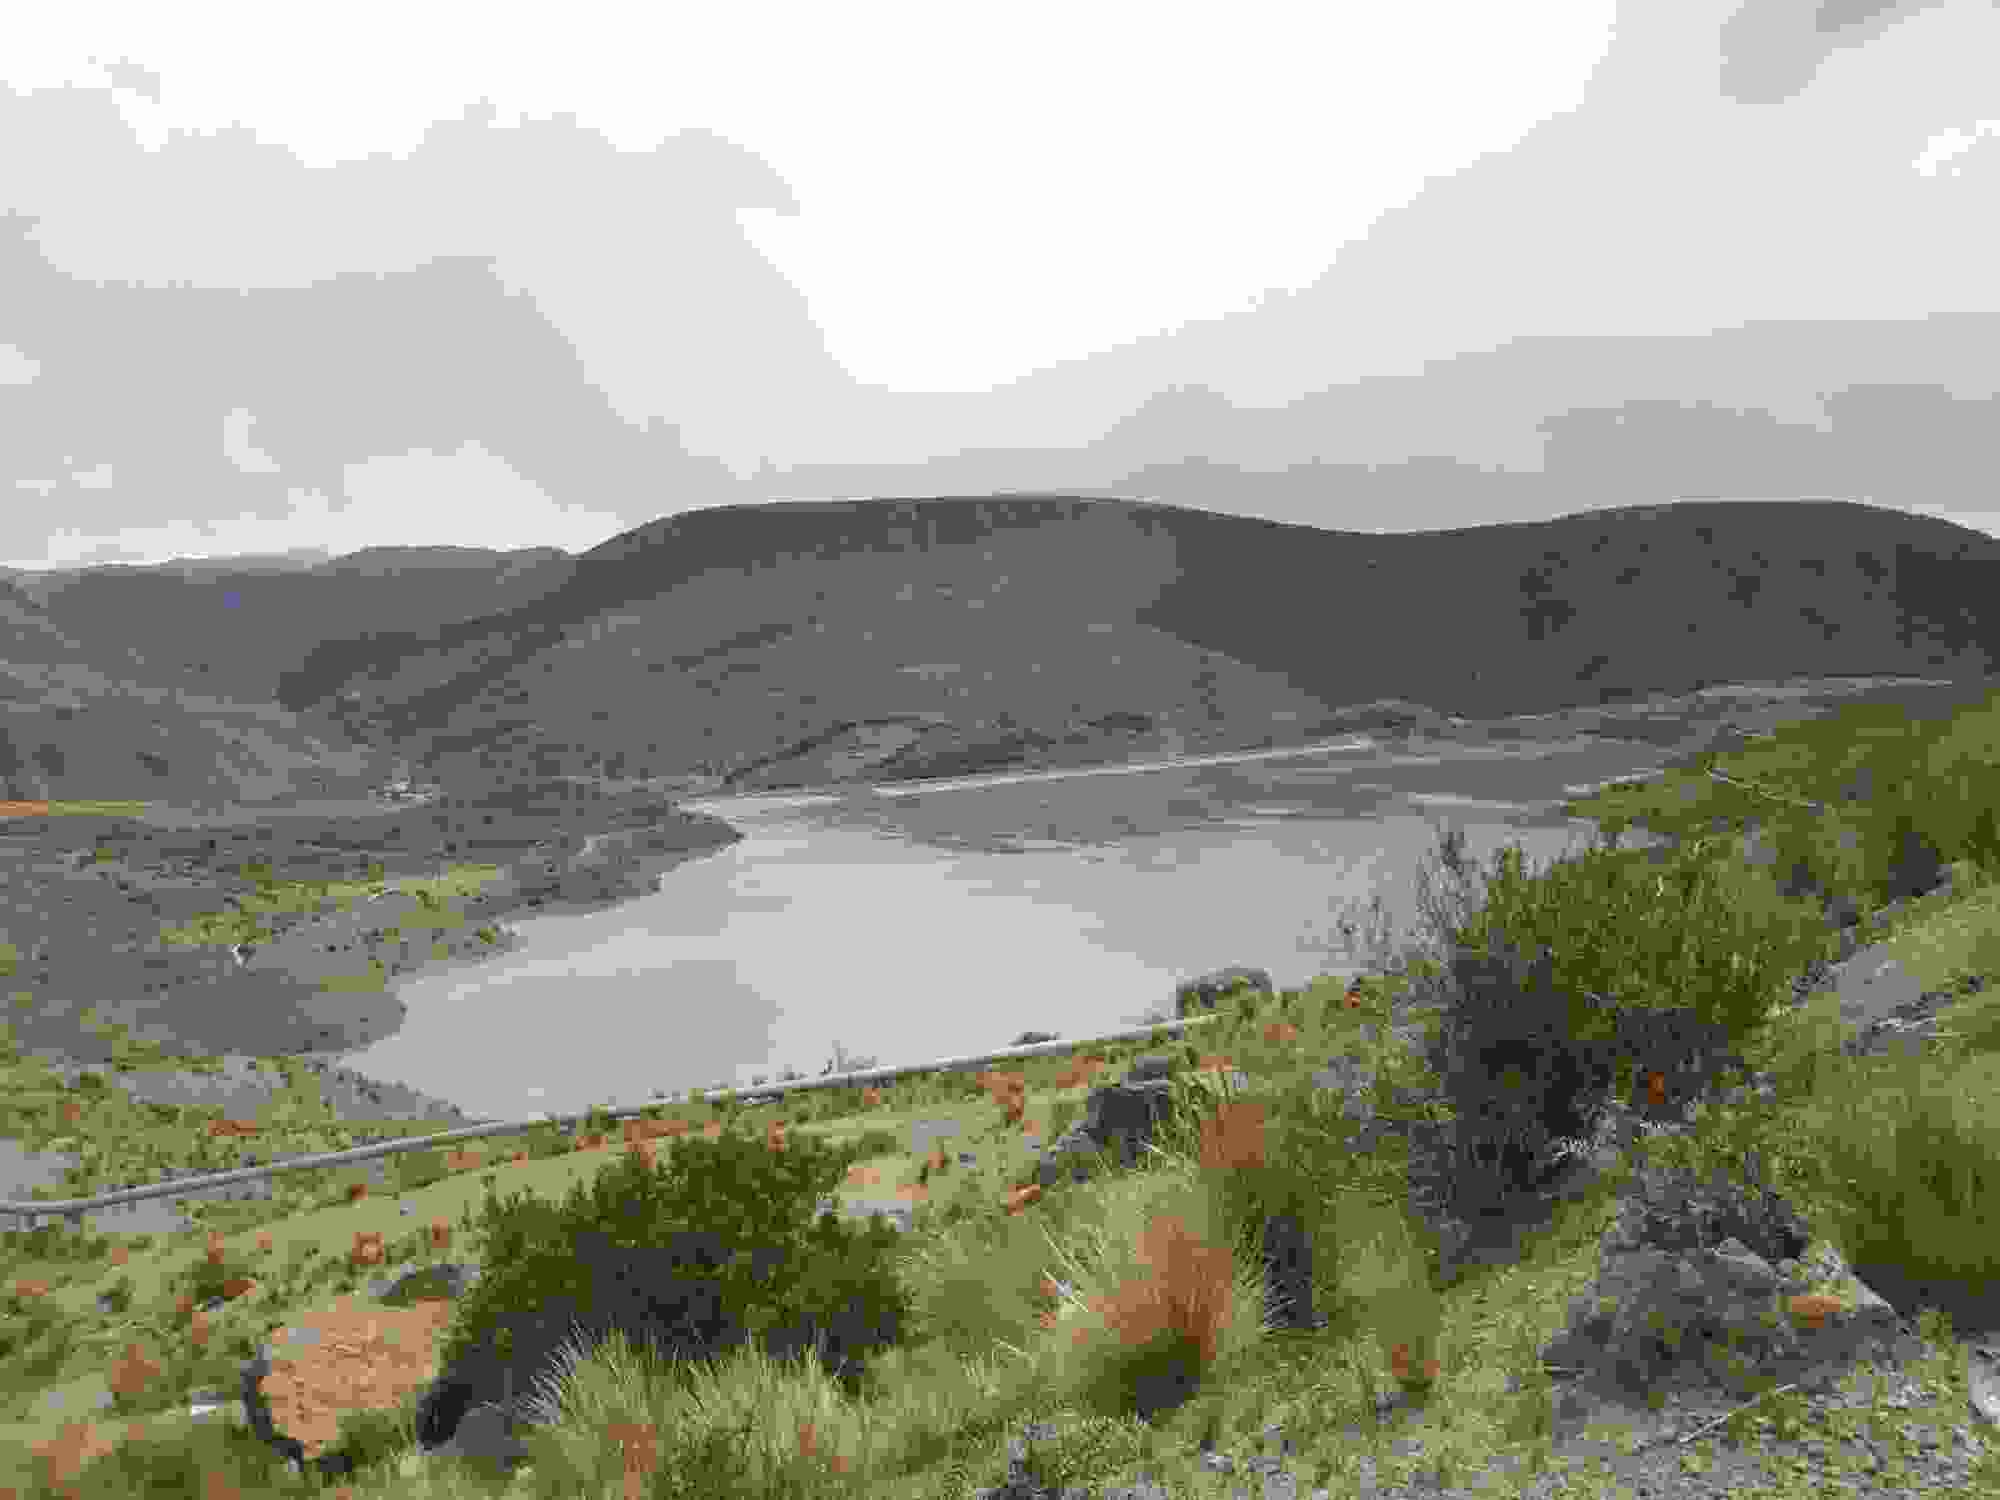
\includegraphics[width=\mywidth]{../wp-content/uploads/2015/04/wpid-wp-1428891087219.jpg} \end{center}

 Le centre de Potosí, des petites rues animées et polluées. 
\begin{center} 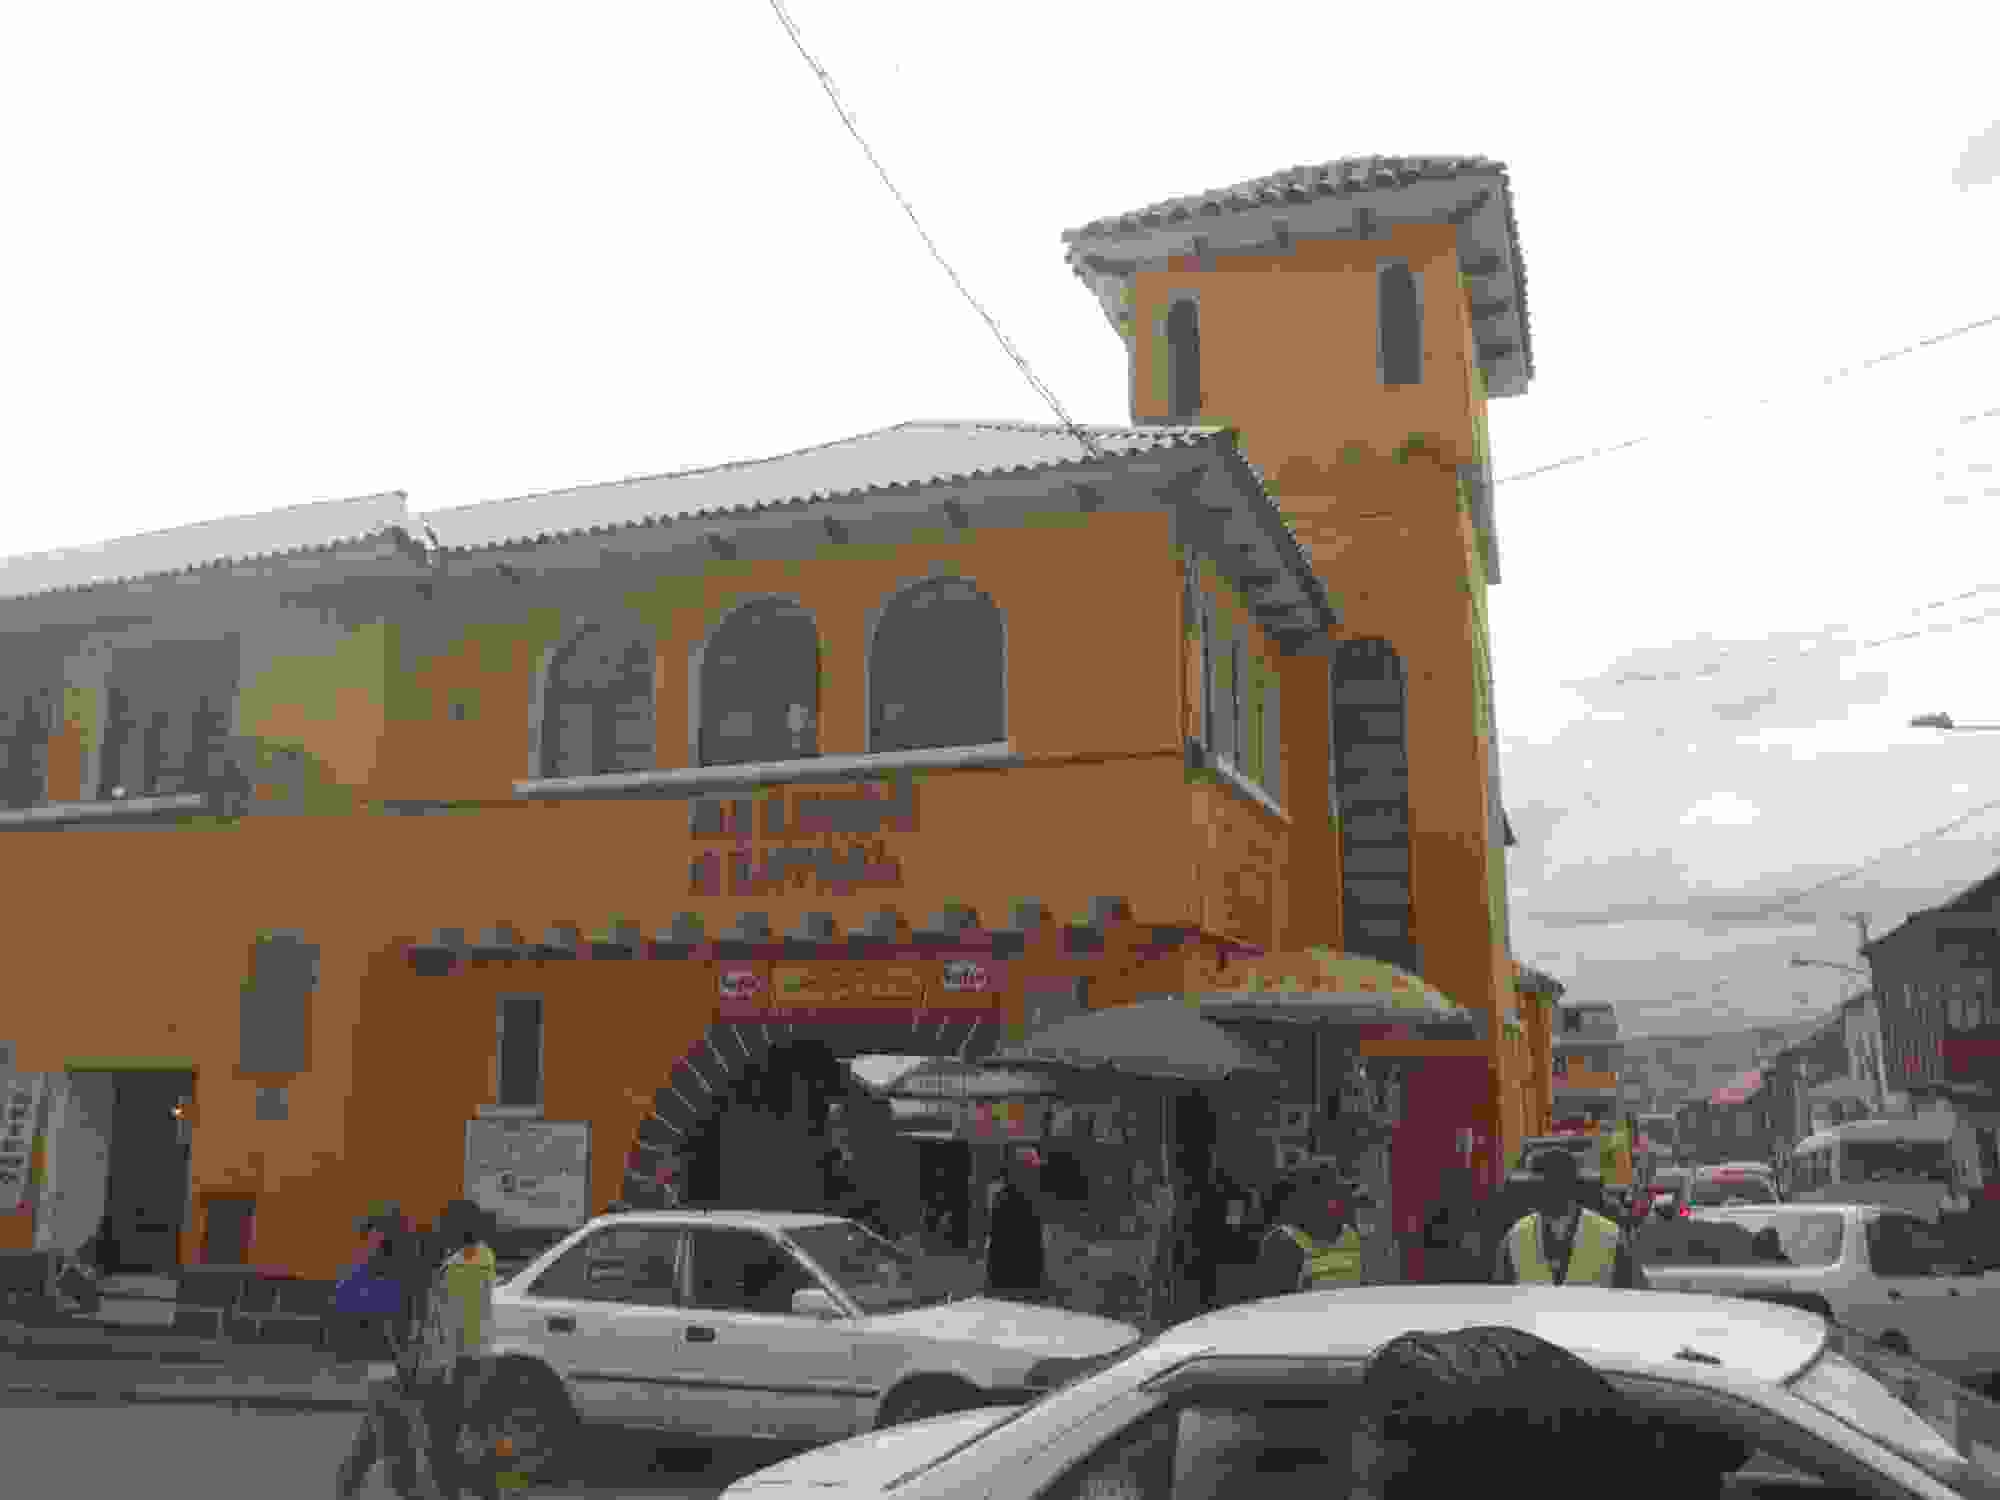
\includegraphics[width=\mywidth]{../wp-content/uploads/2015/04/wpid-wp-1428891137998.jpg} \end{center}
\vspace{-\topsep}

\pagebreak
~\\
\begin{center} 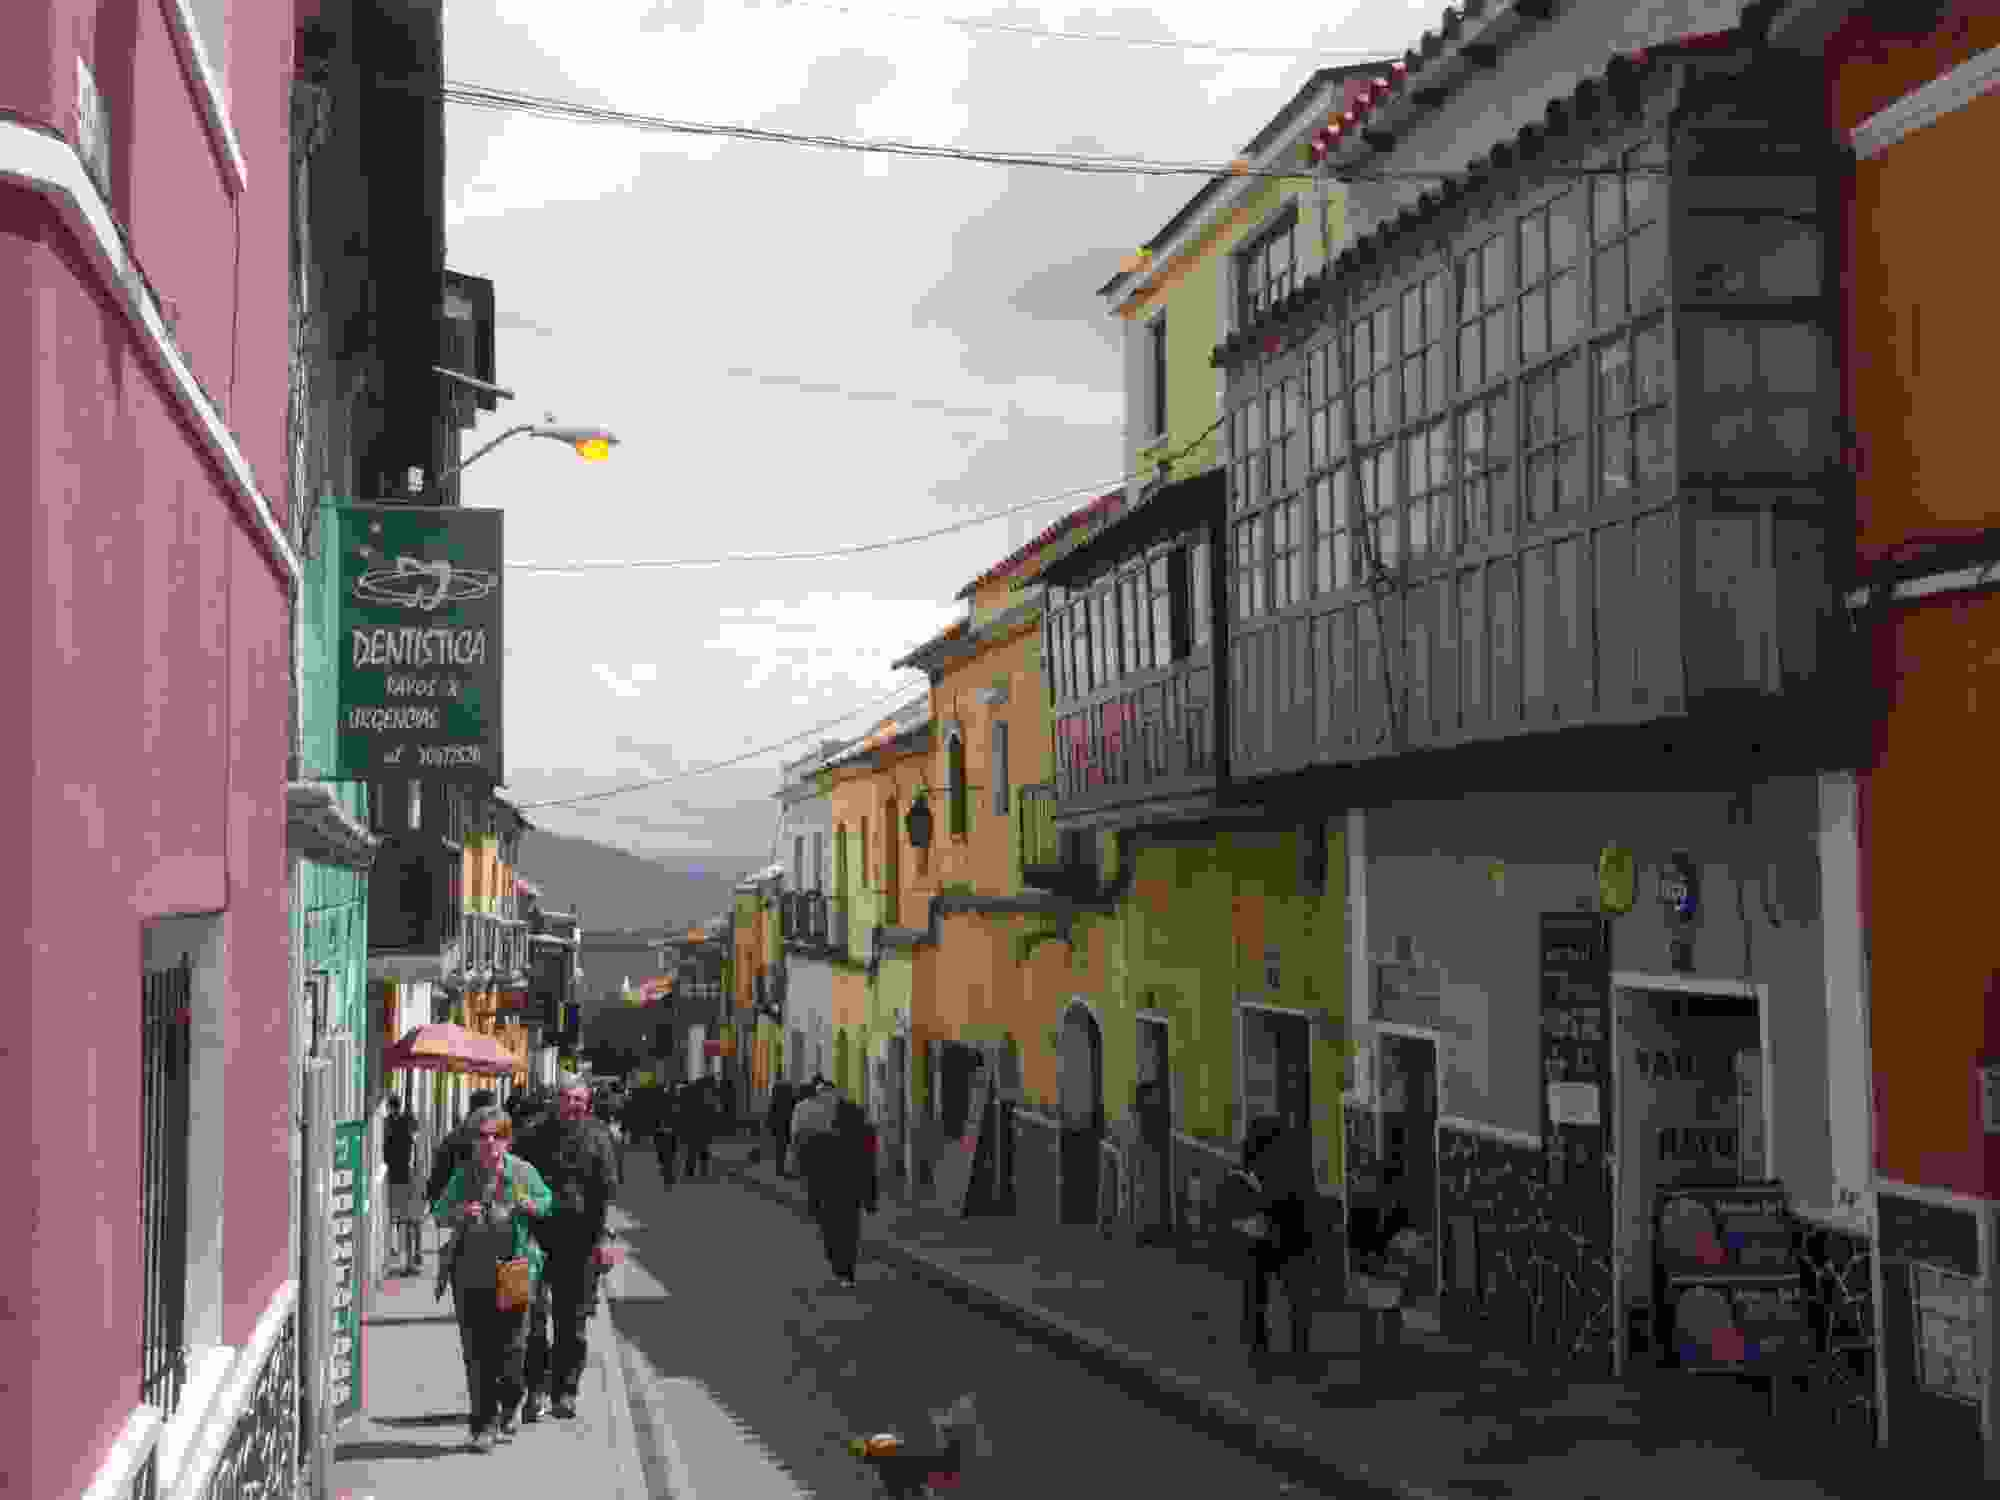
\includegraphics[width=\mywidth]{../wp-content/uploads/2015/04/wpid-wp-1428891177251.jpg} \end{center}
~
\begin{center} 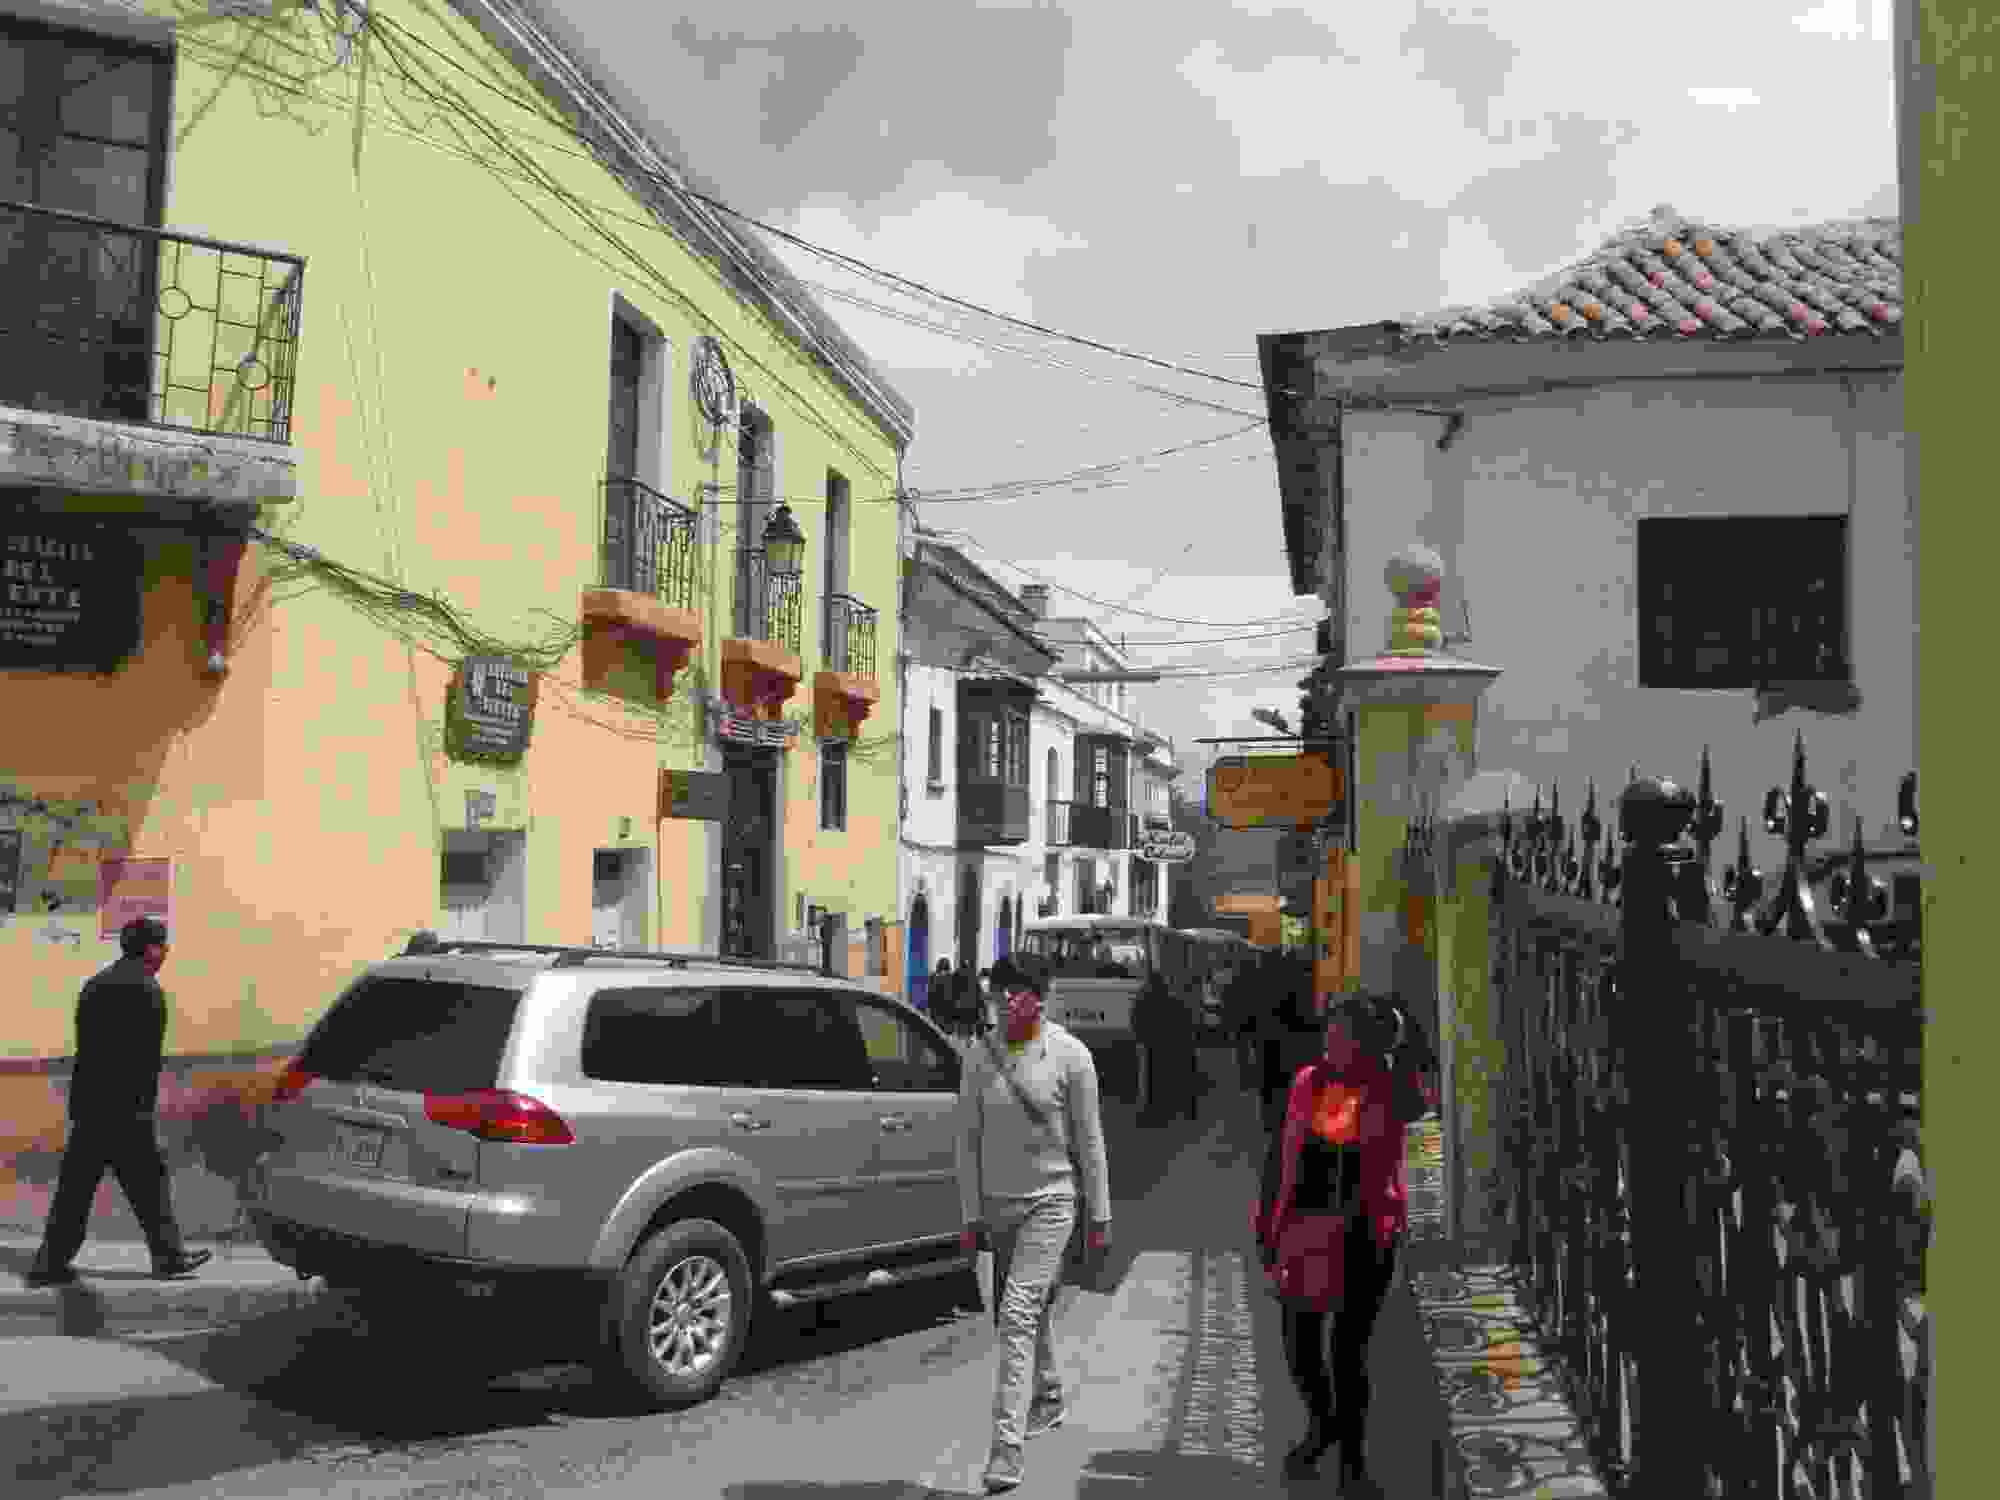
\includegraphics[width=\mywidth]{../wp-content/uploads/2015/04/wpid-wp-1428891217403.jpg} \end{center}
\vspace{-\topsep}

\pagebreak
  La cathédrale :
\begin{center} 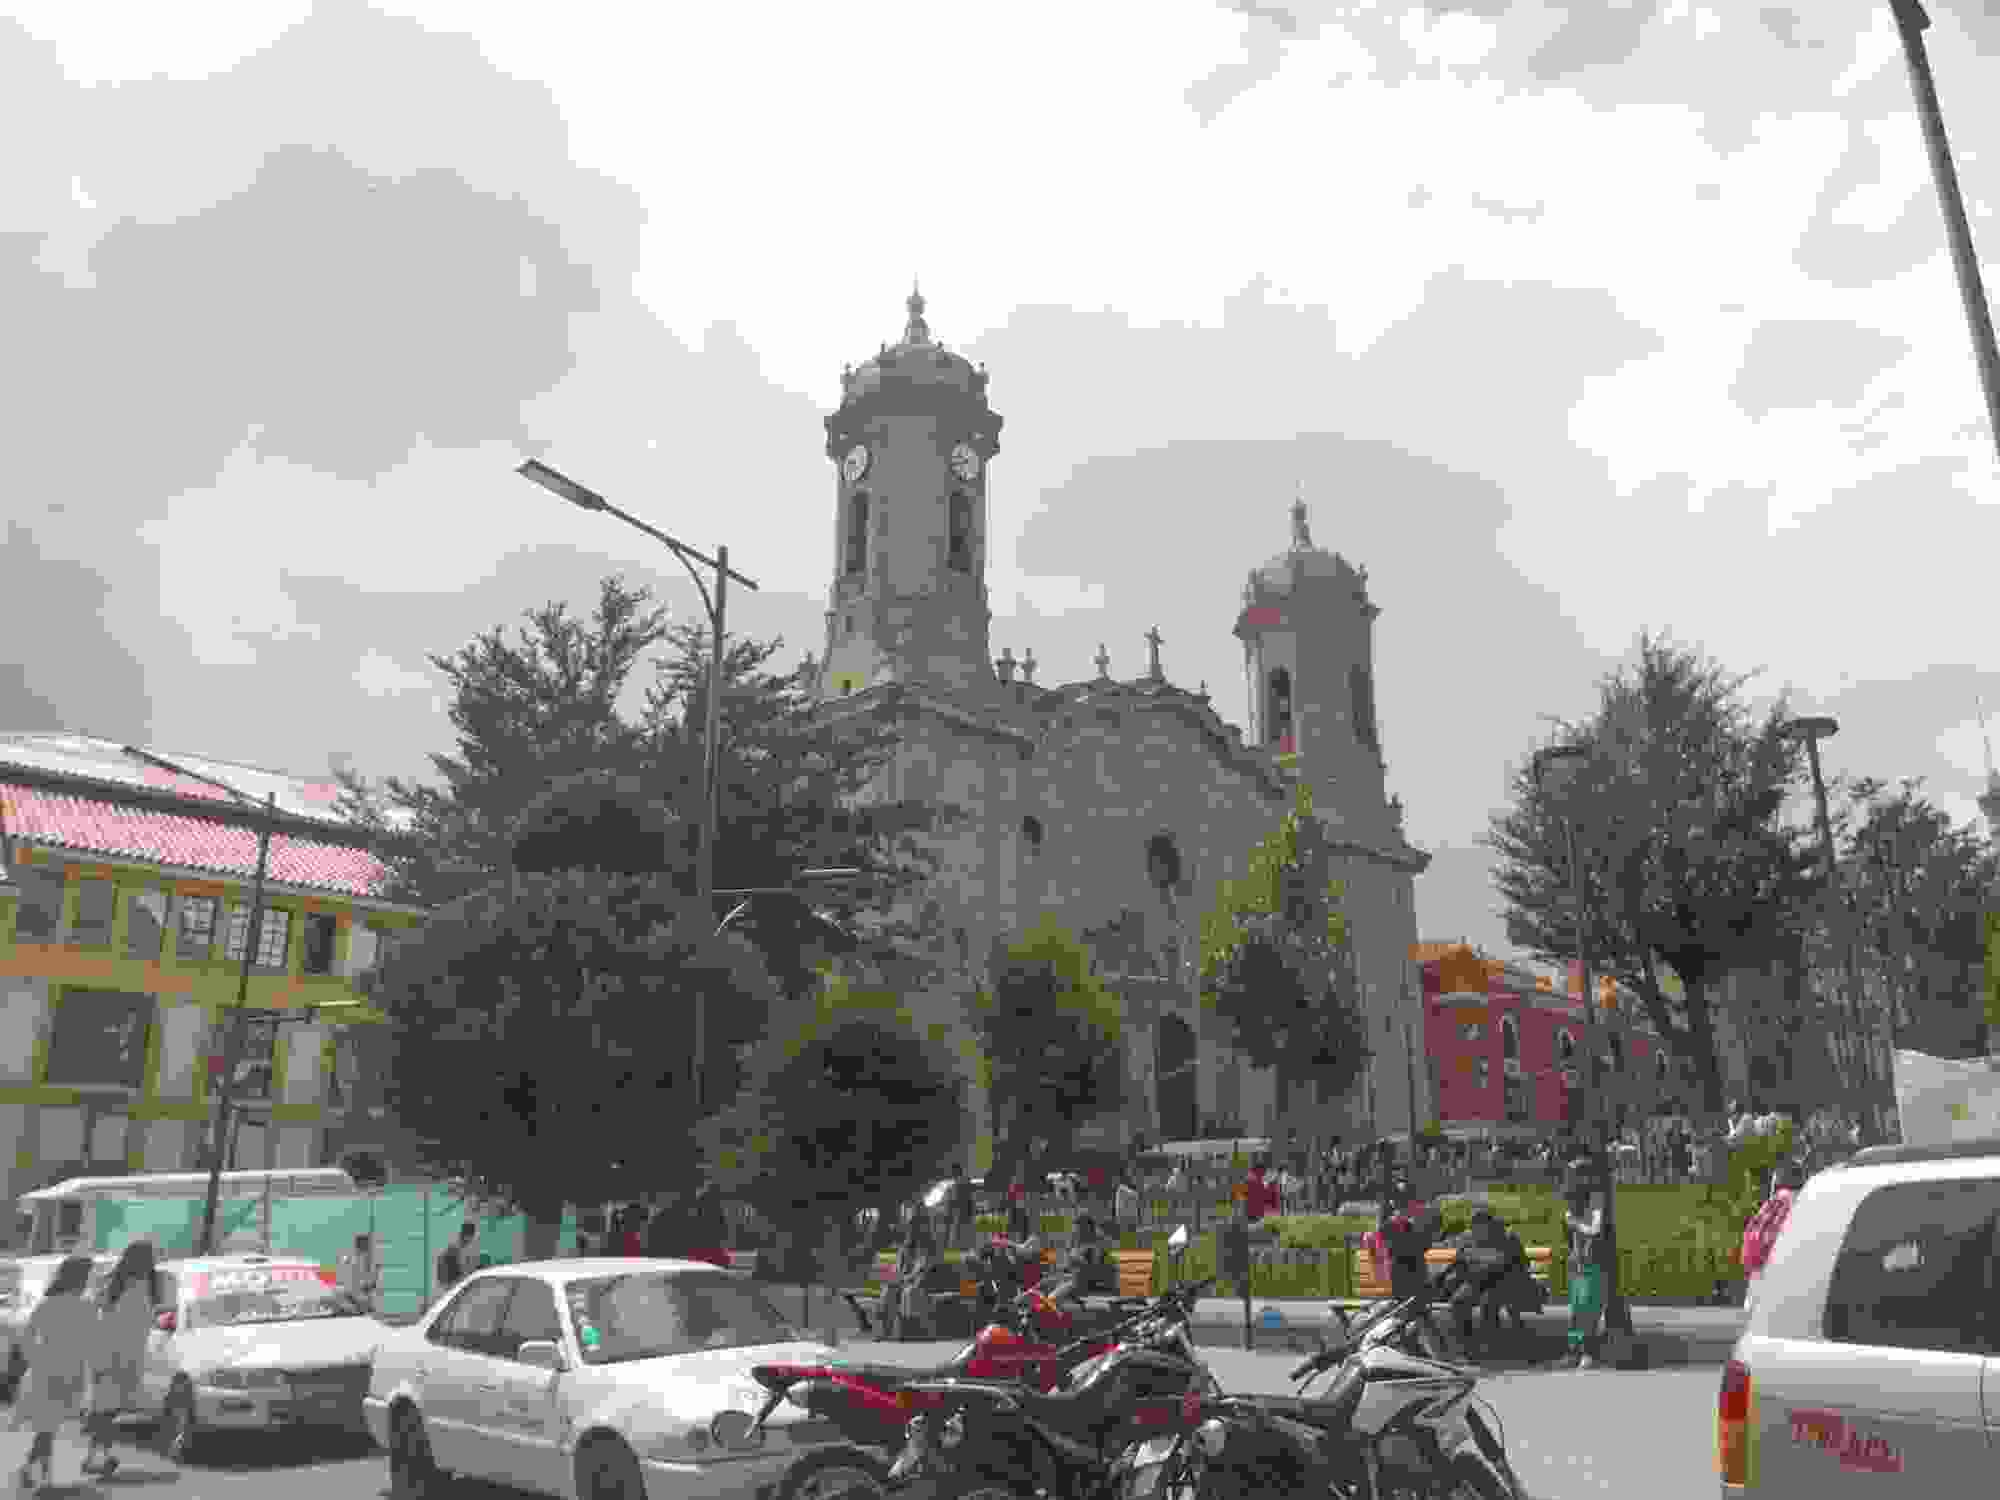
\includegraphics[width=\mywidth]{../wp-content/uploads/2015/04/wpid-wp-1428891310502.jpg} \end{center}

  Une église :
\begin{center} 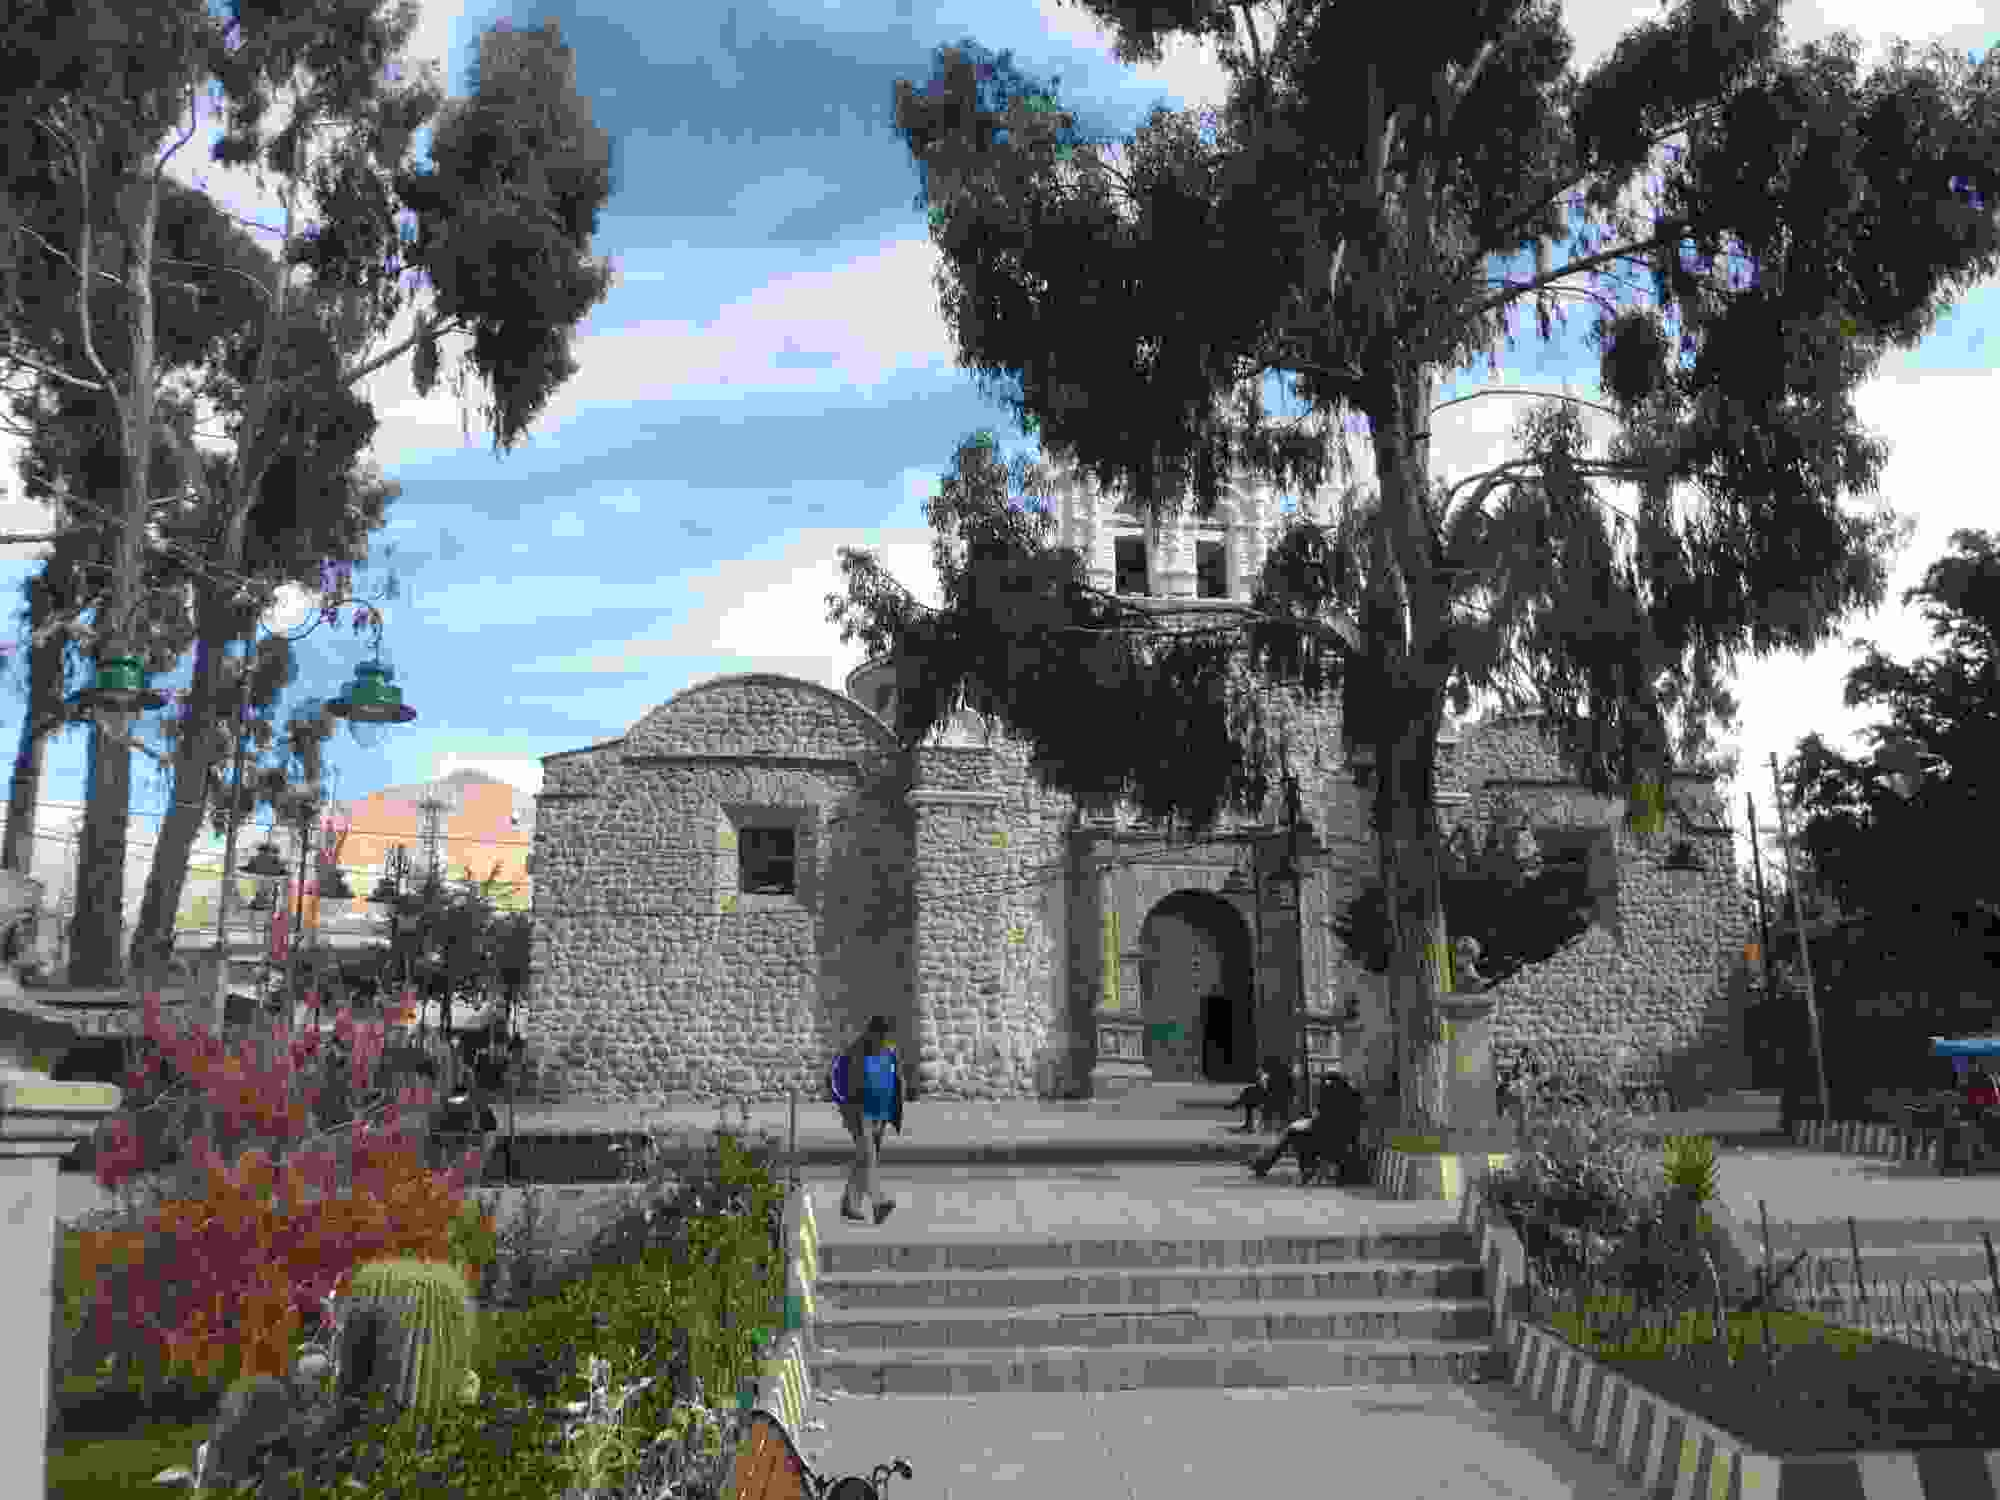
\includegraphics[width=\mywidth]{../wp-content/uploads/2015/04/wpid-wp-1428891346885.jpg} \end{center}

 Le couvent Santa Teresa, visite guidée intéressante sur la vie des soeurs à l'époque coloniale : une fois entrées à l'âge de 15 ans celles-ci étaient cloîtrées le reste de leur vie sans aucun contact avec l'extérieur. 
\begin{center} 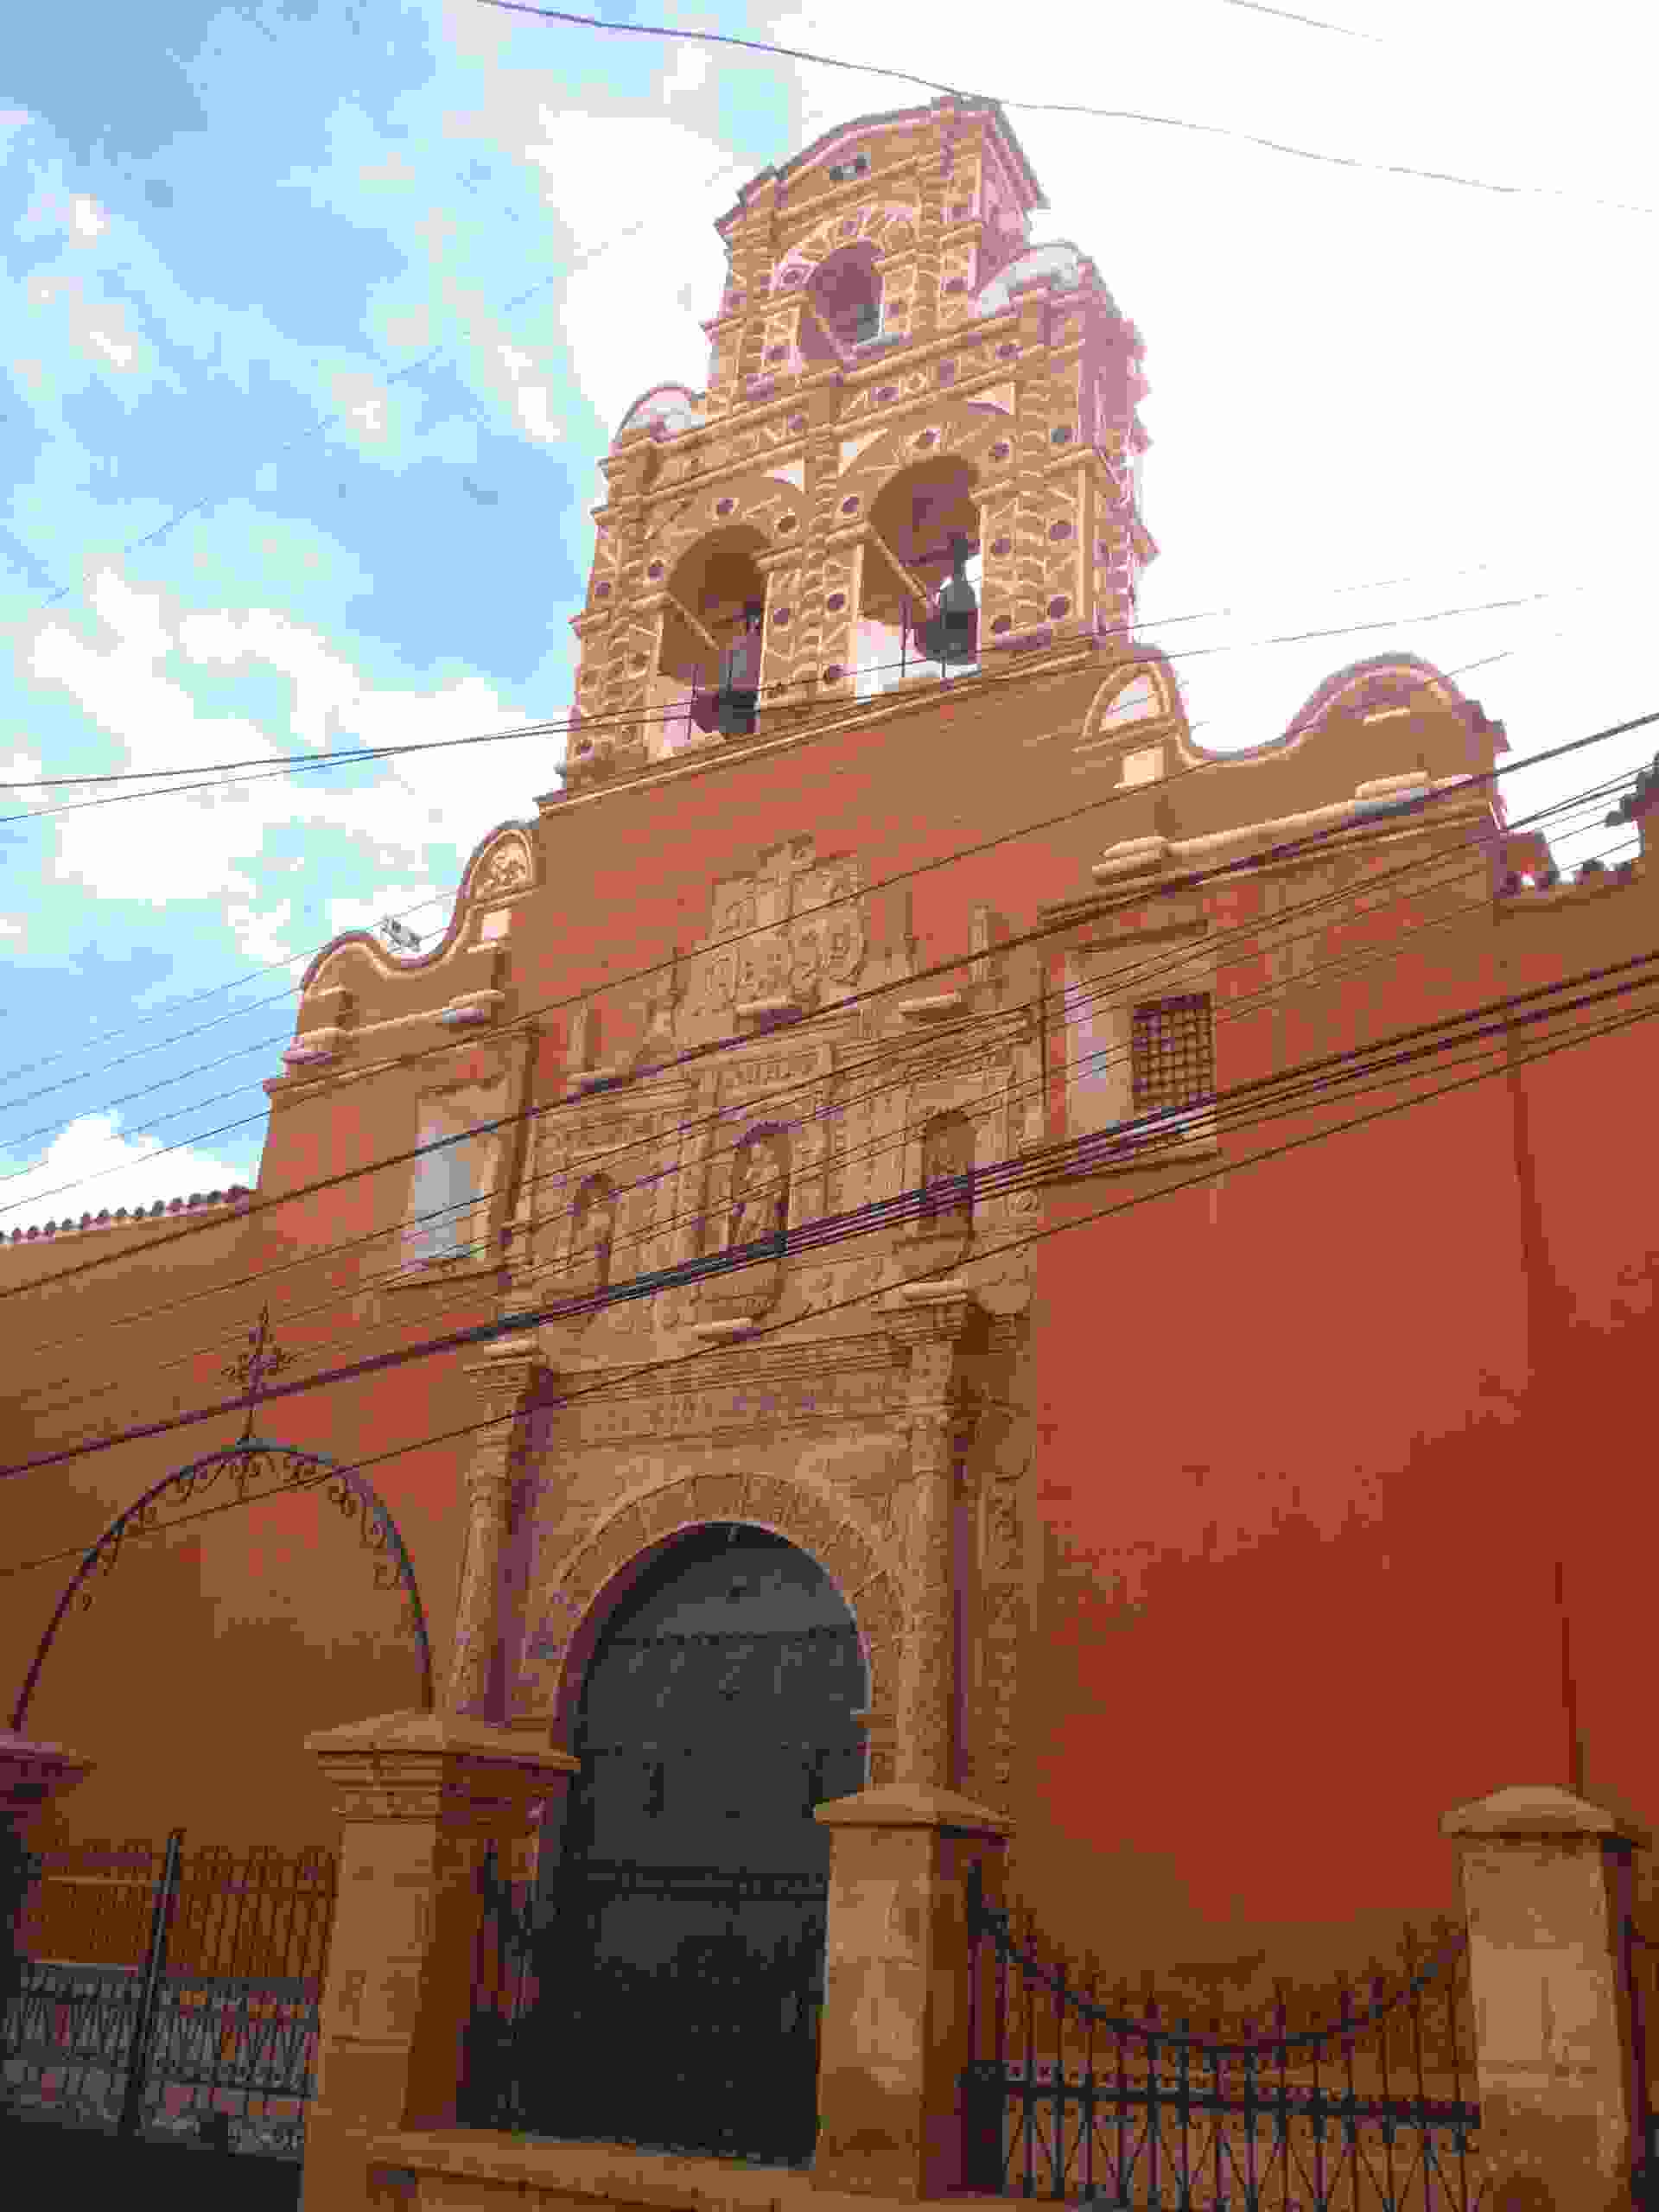
\includegraphics[height=\mywidth]{../wp-content/uploads/2015/04/wpid-wp-1428891737578.jpg} \end{center}

 La Casa de la Moneda :
\begin{center} 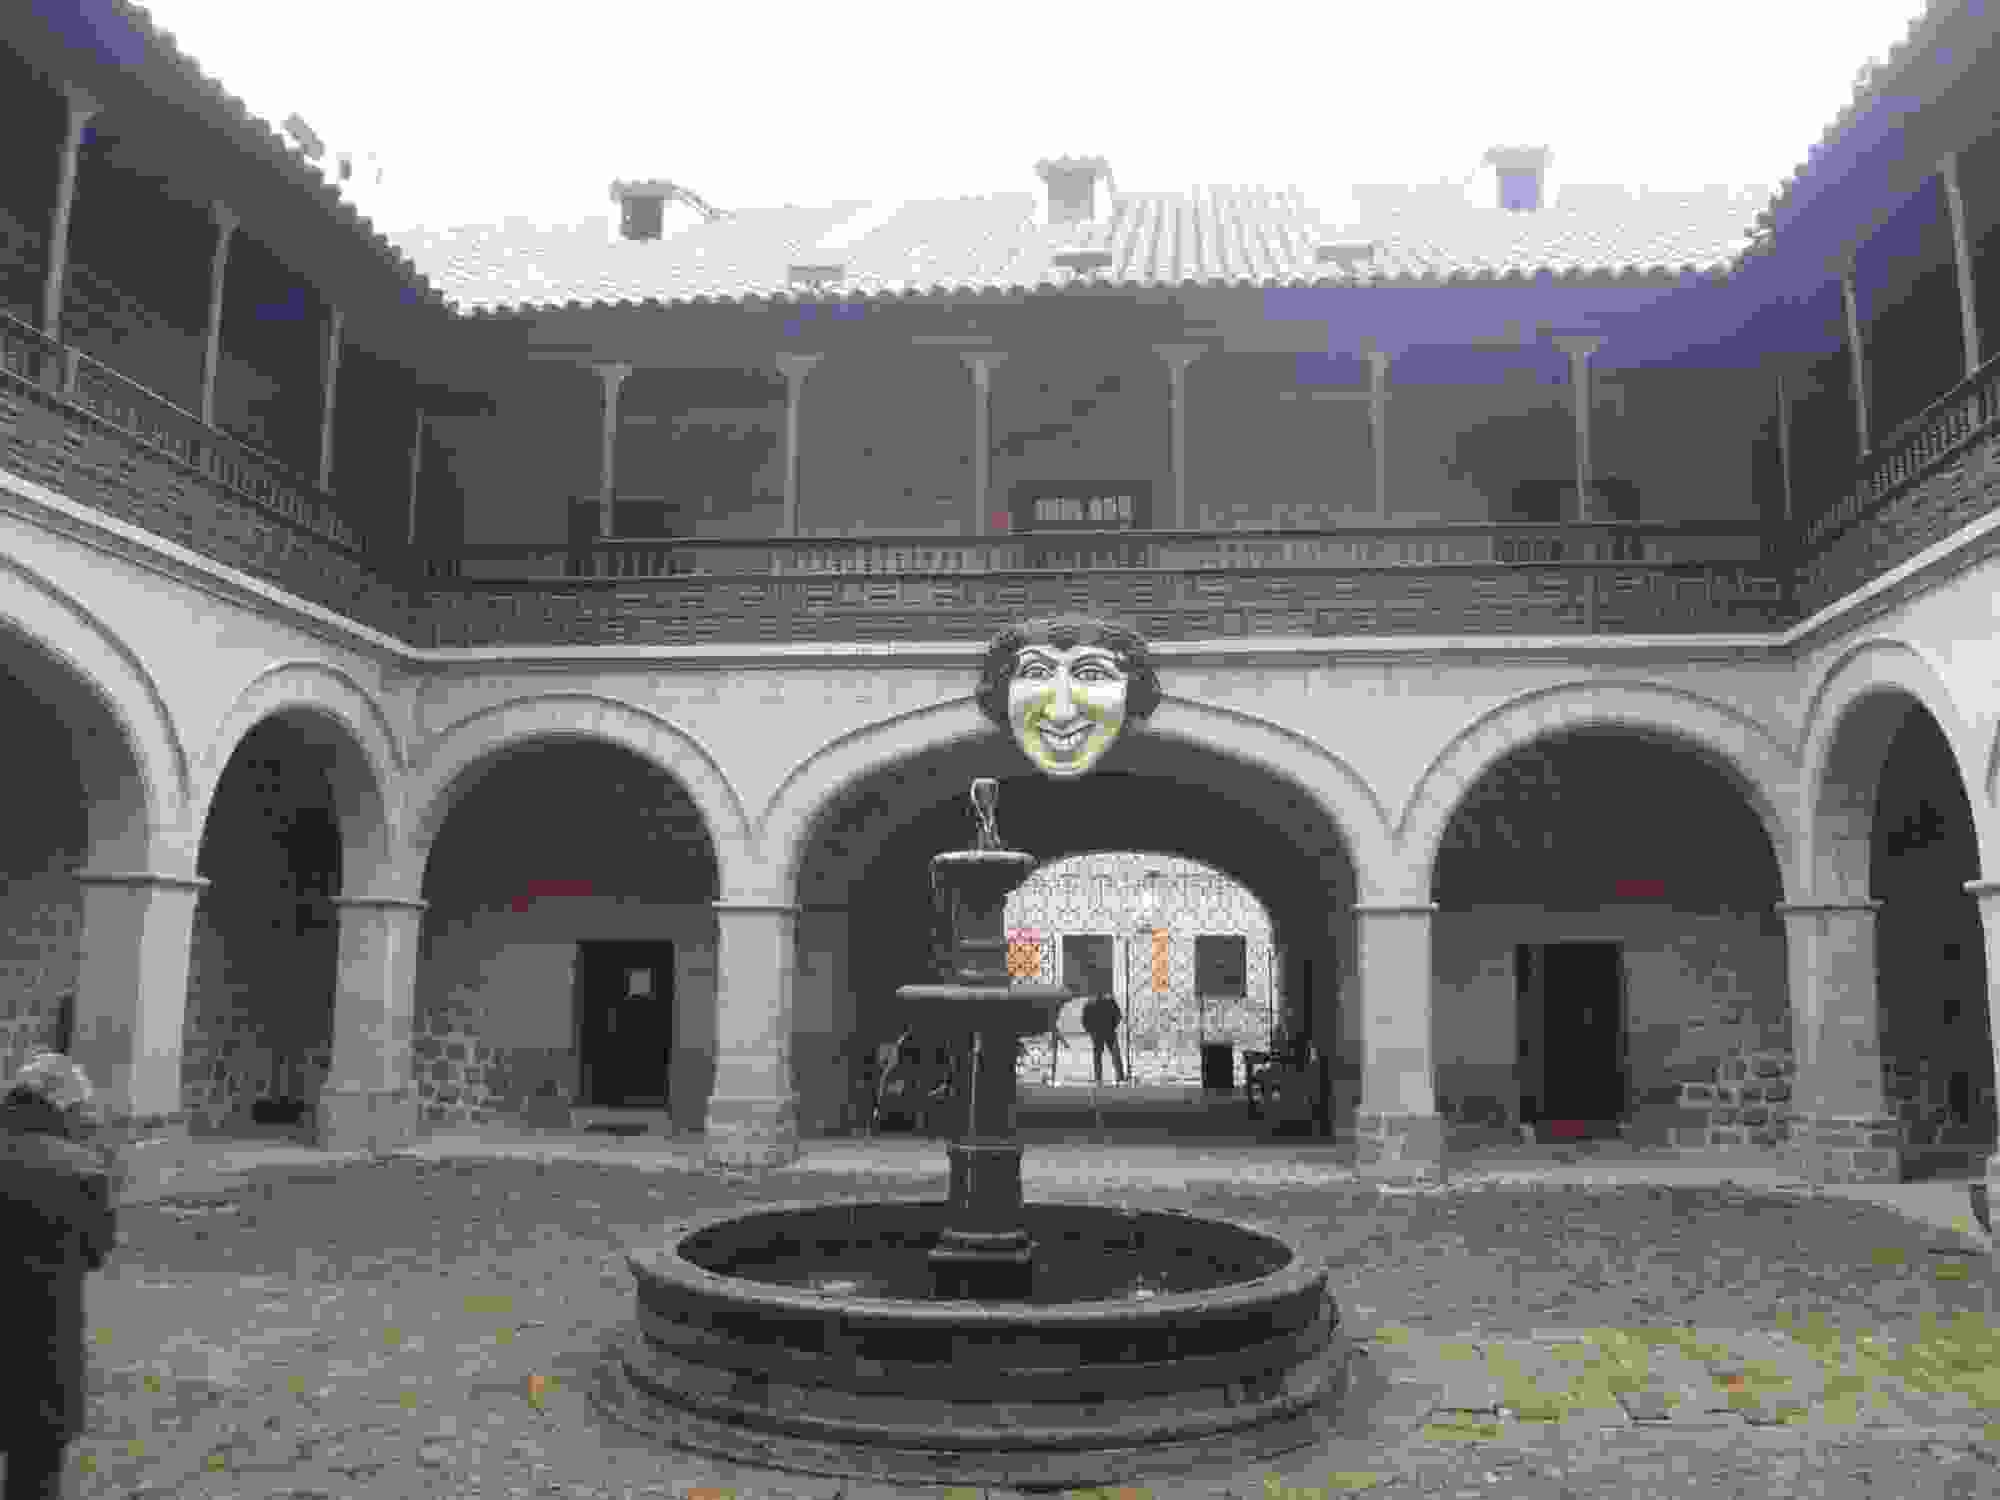
\includegraphics[width=\mywidth]{../wp-content/uploads/2015/04/wpid-wp-1428891875565.jpg} \end{center}

 Mais Potosí ce sont avant tout les mines d'argent, creusées dans le Cerro Rico.
\begin{center} 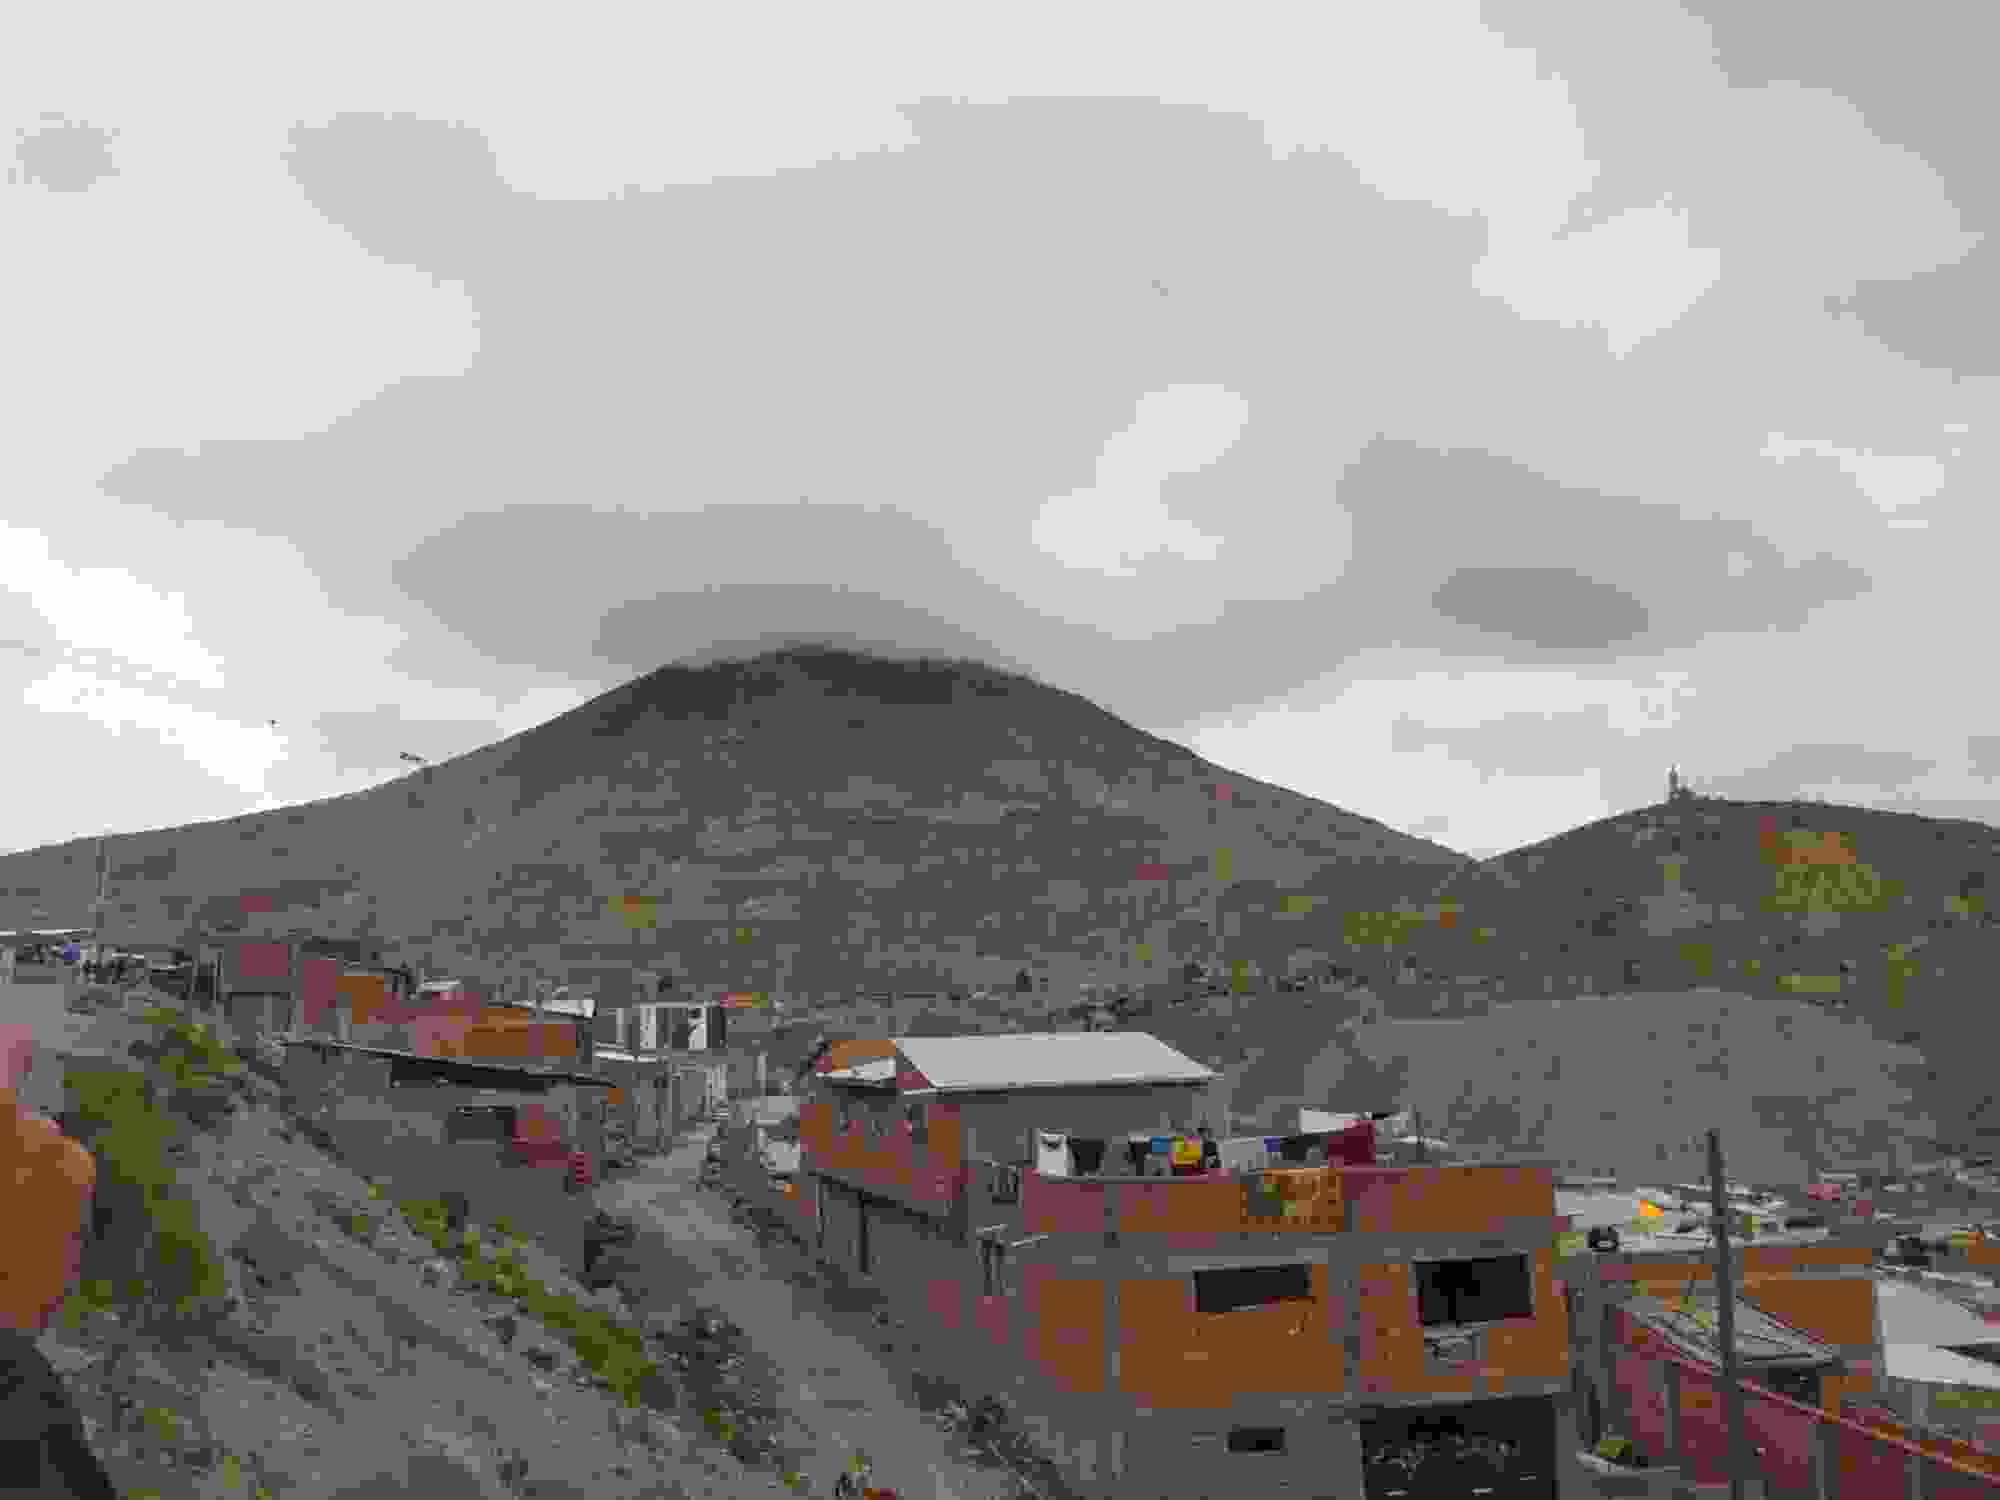
\includegraphics[width=\mywidth]{../wp-content/uploads/2015/04/wpid-wp-1428891958963.jpg} \end{center}

 La visite commence au marché des mineurs pour acheter des cadeaux pour les mineurs : feuilles de coca, boissons.
\begin{center} 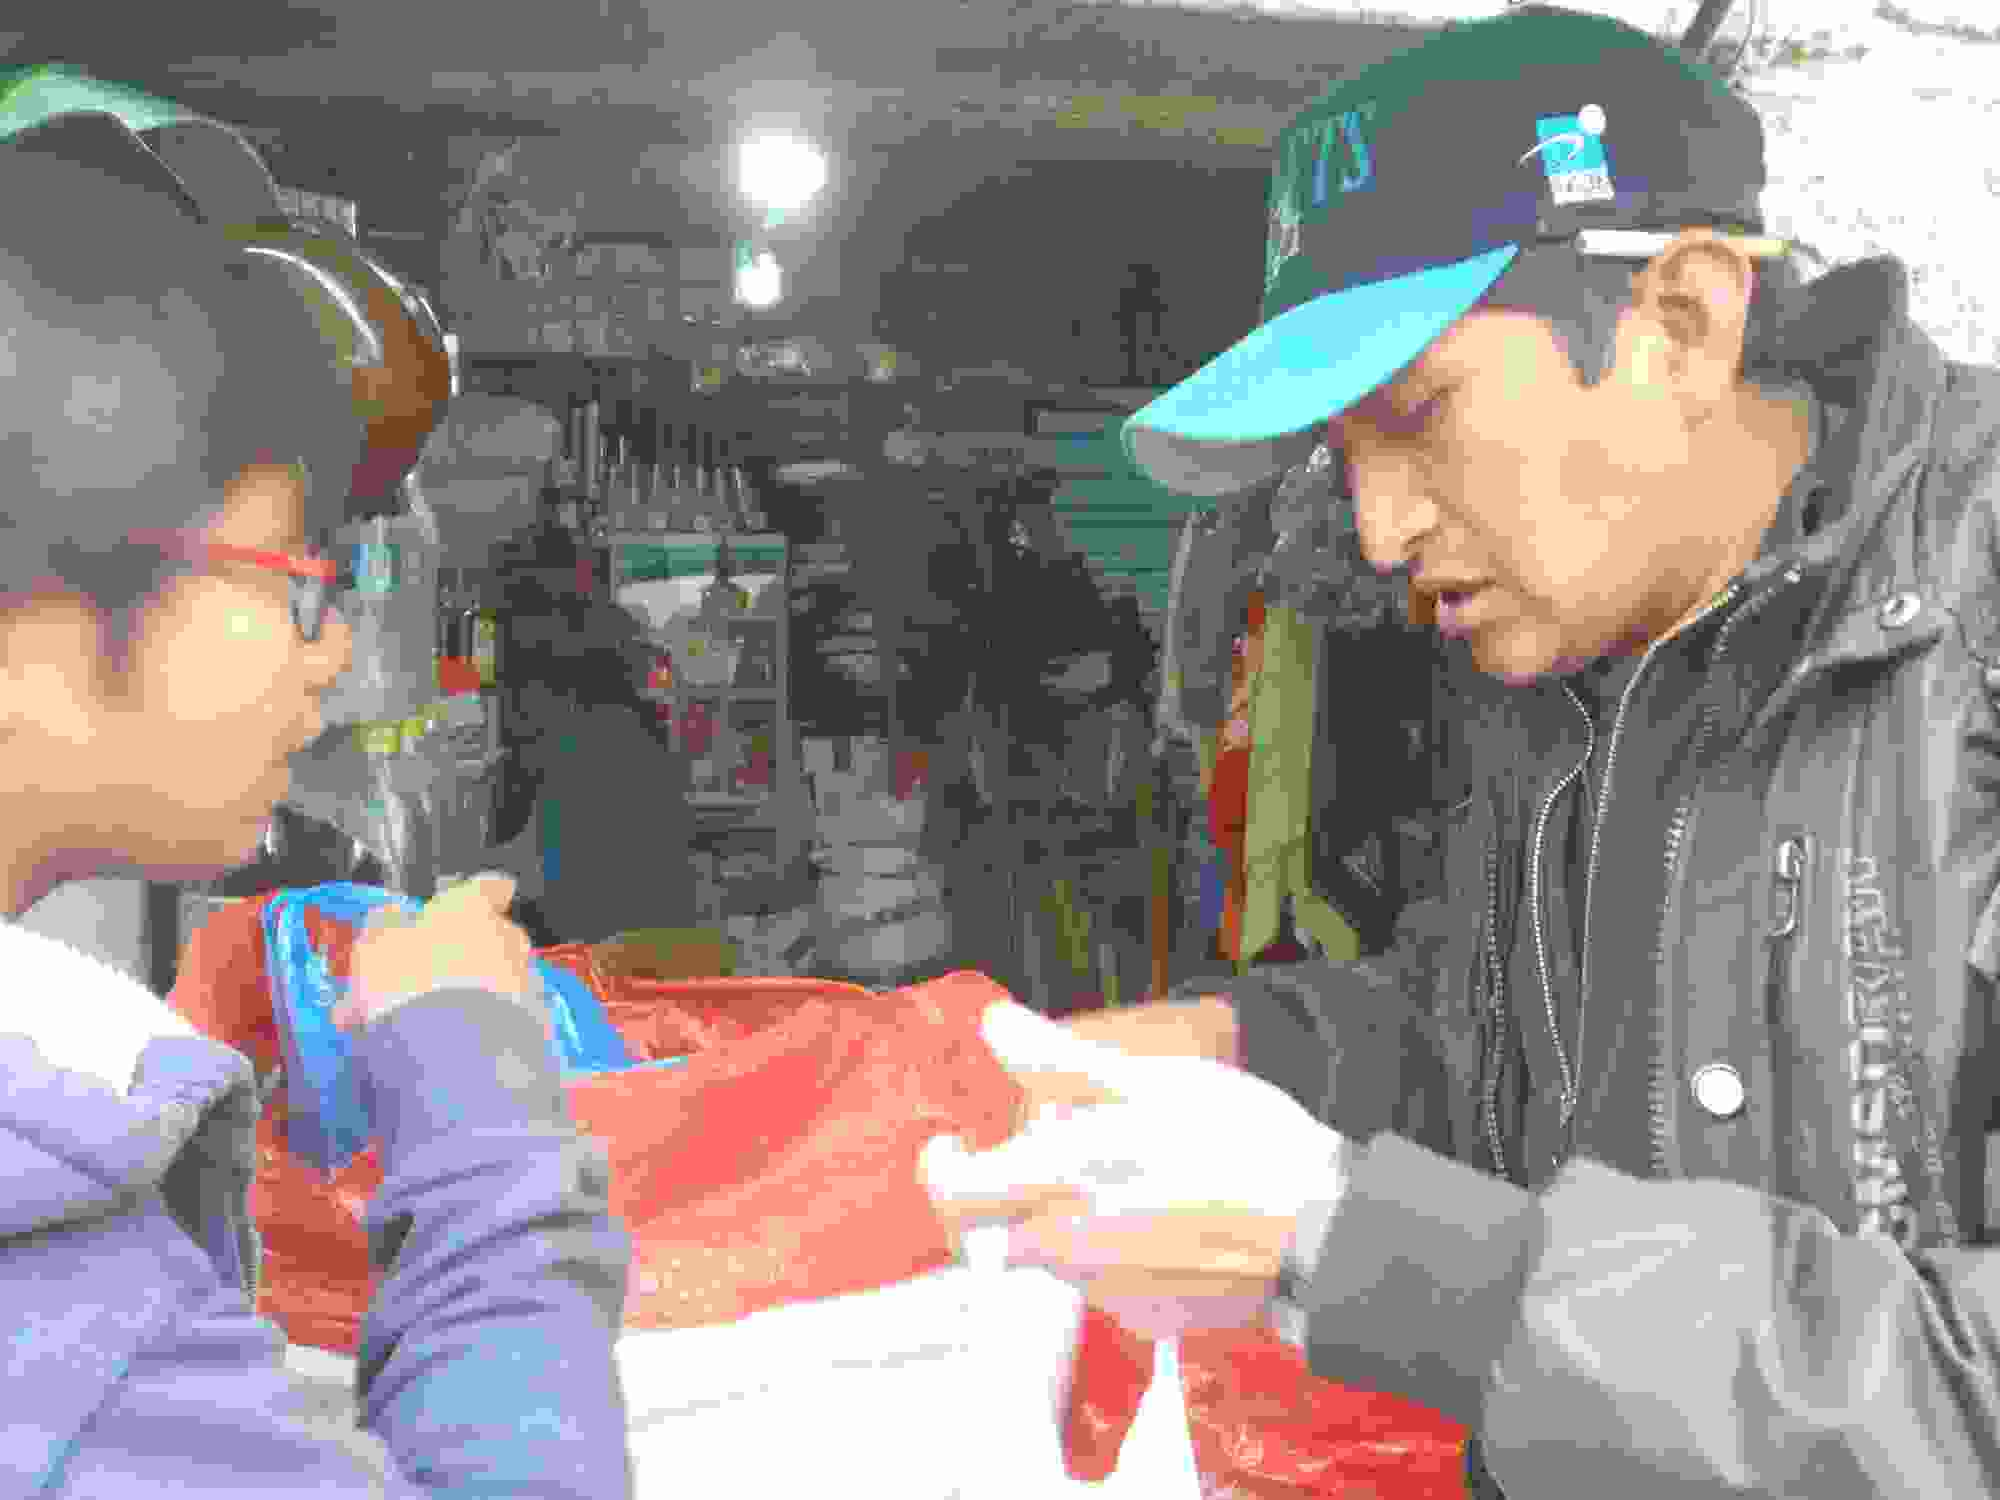
\includegraphics[width=\mywidth]{../wp-content/uploads/2015/04/wpid-wp-1428892276575.jpg} \end{center}
\vspace{-\topsep}

\pagebreak
 On enfile la tenue de protection. \\
\begin{center} 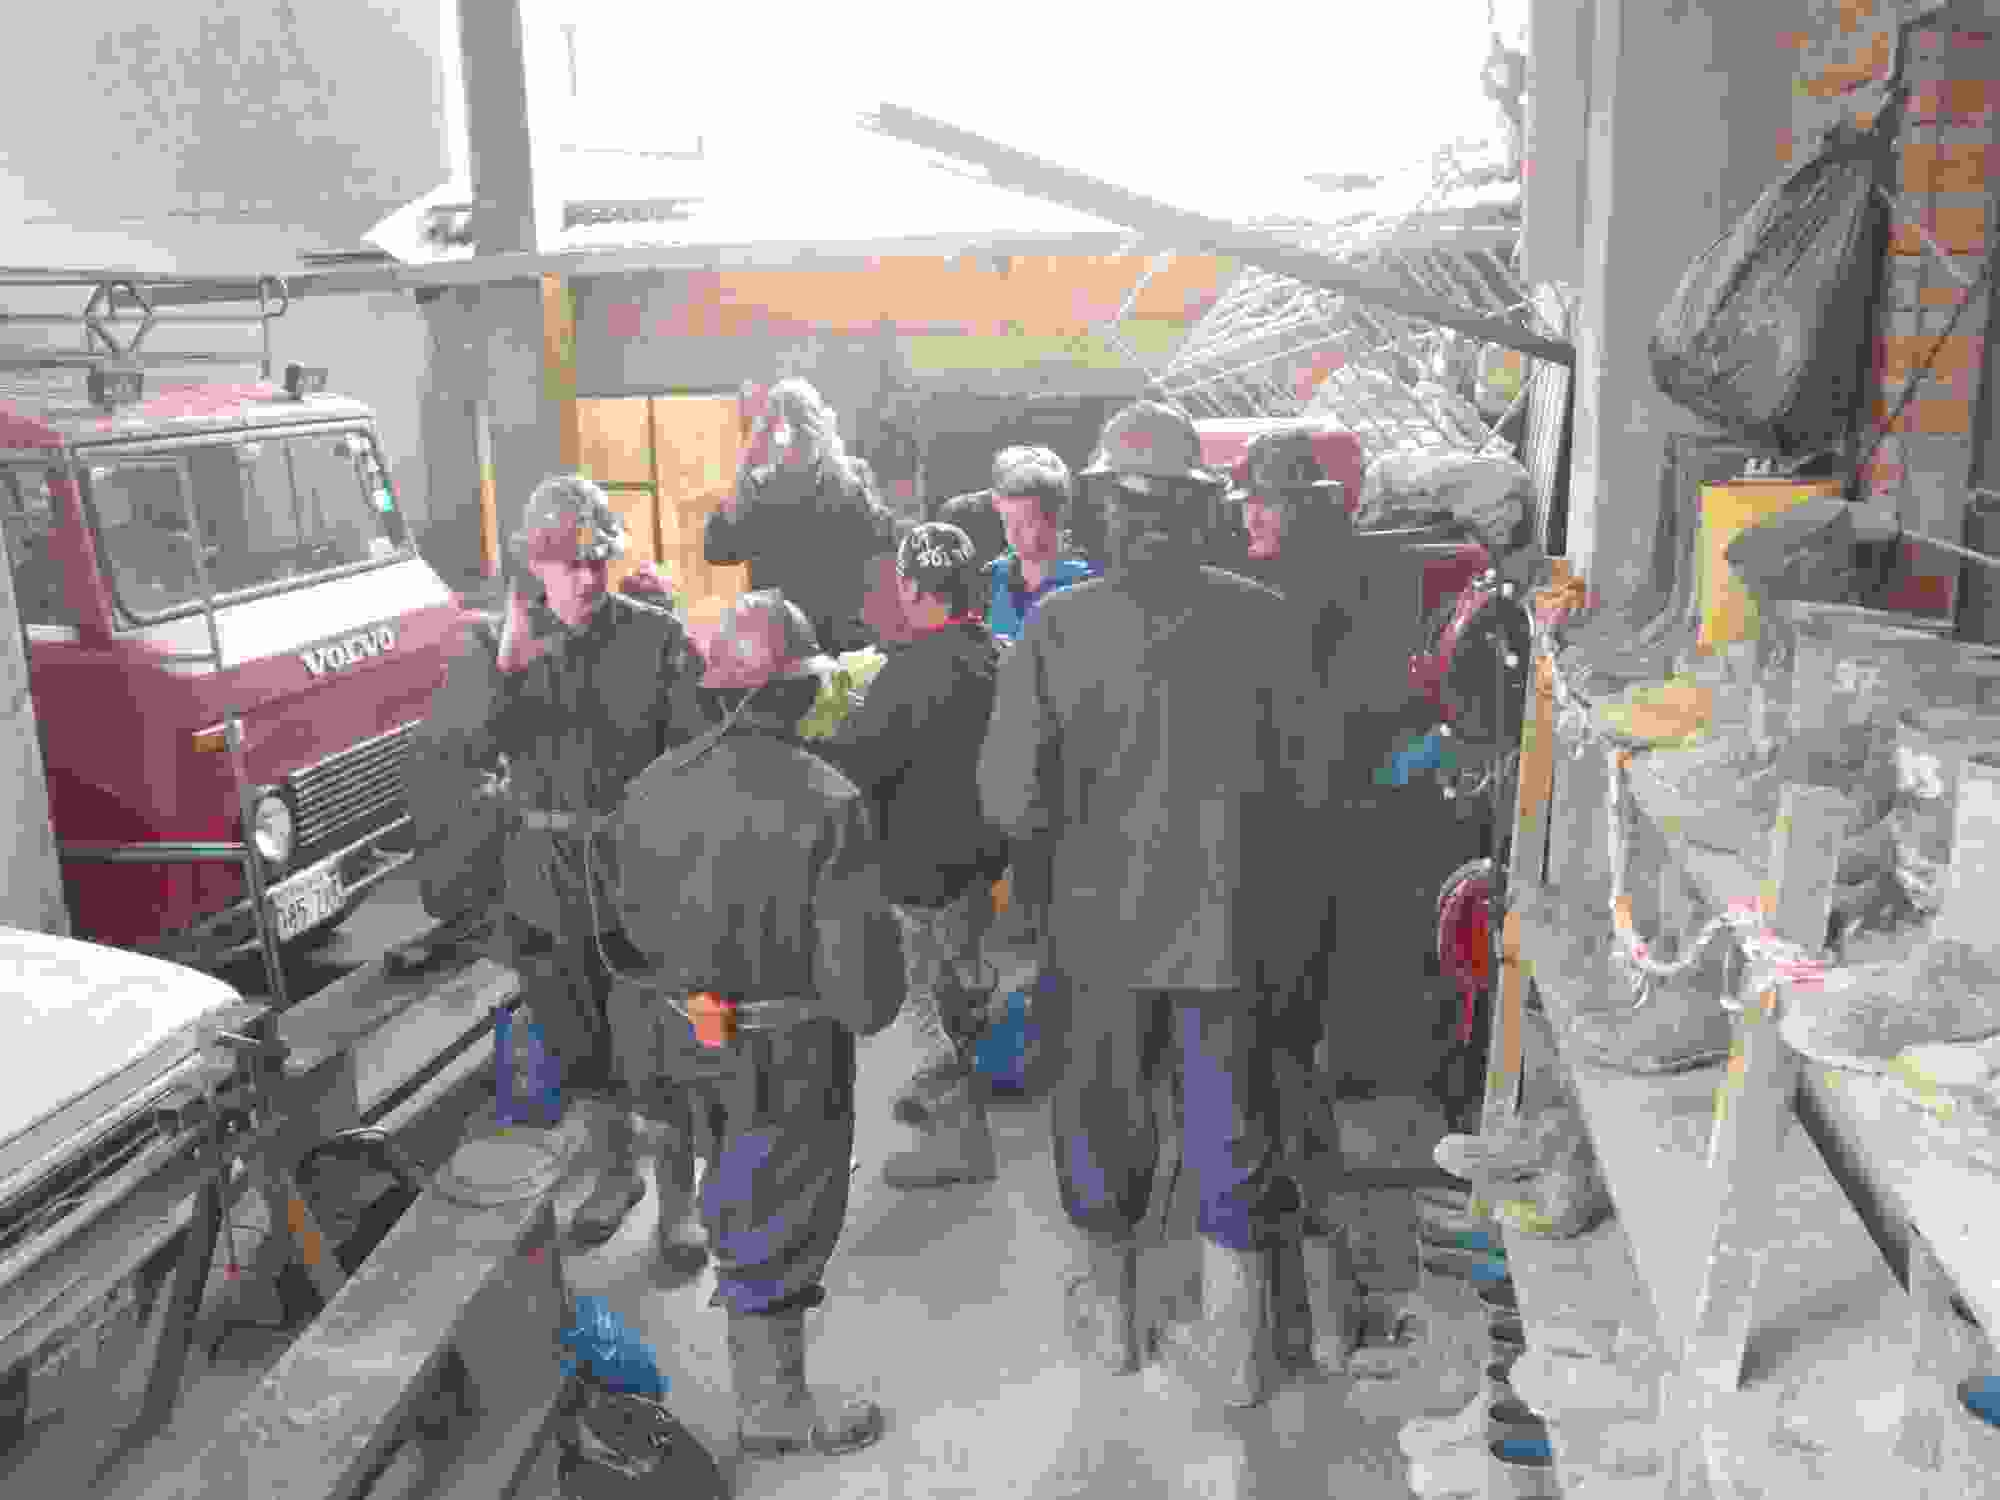
\includegraphics[width=\mywidth]{../wp-content/uploads/2015/04/wpid-wp-1428892402383.jpg} \end{center}

 Visite d'une usine de traitement des minerais : argent, zinc et plomb sont extraits ici. 
\begin{center} 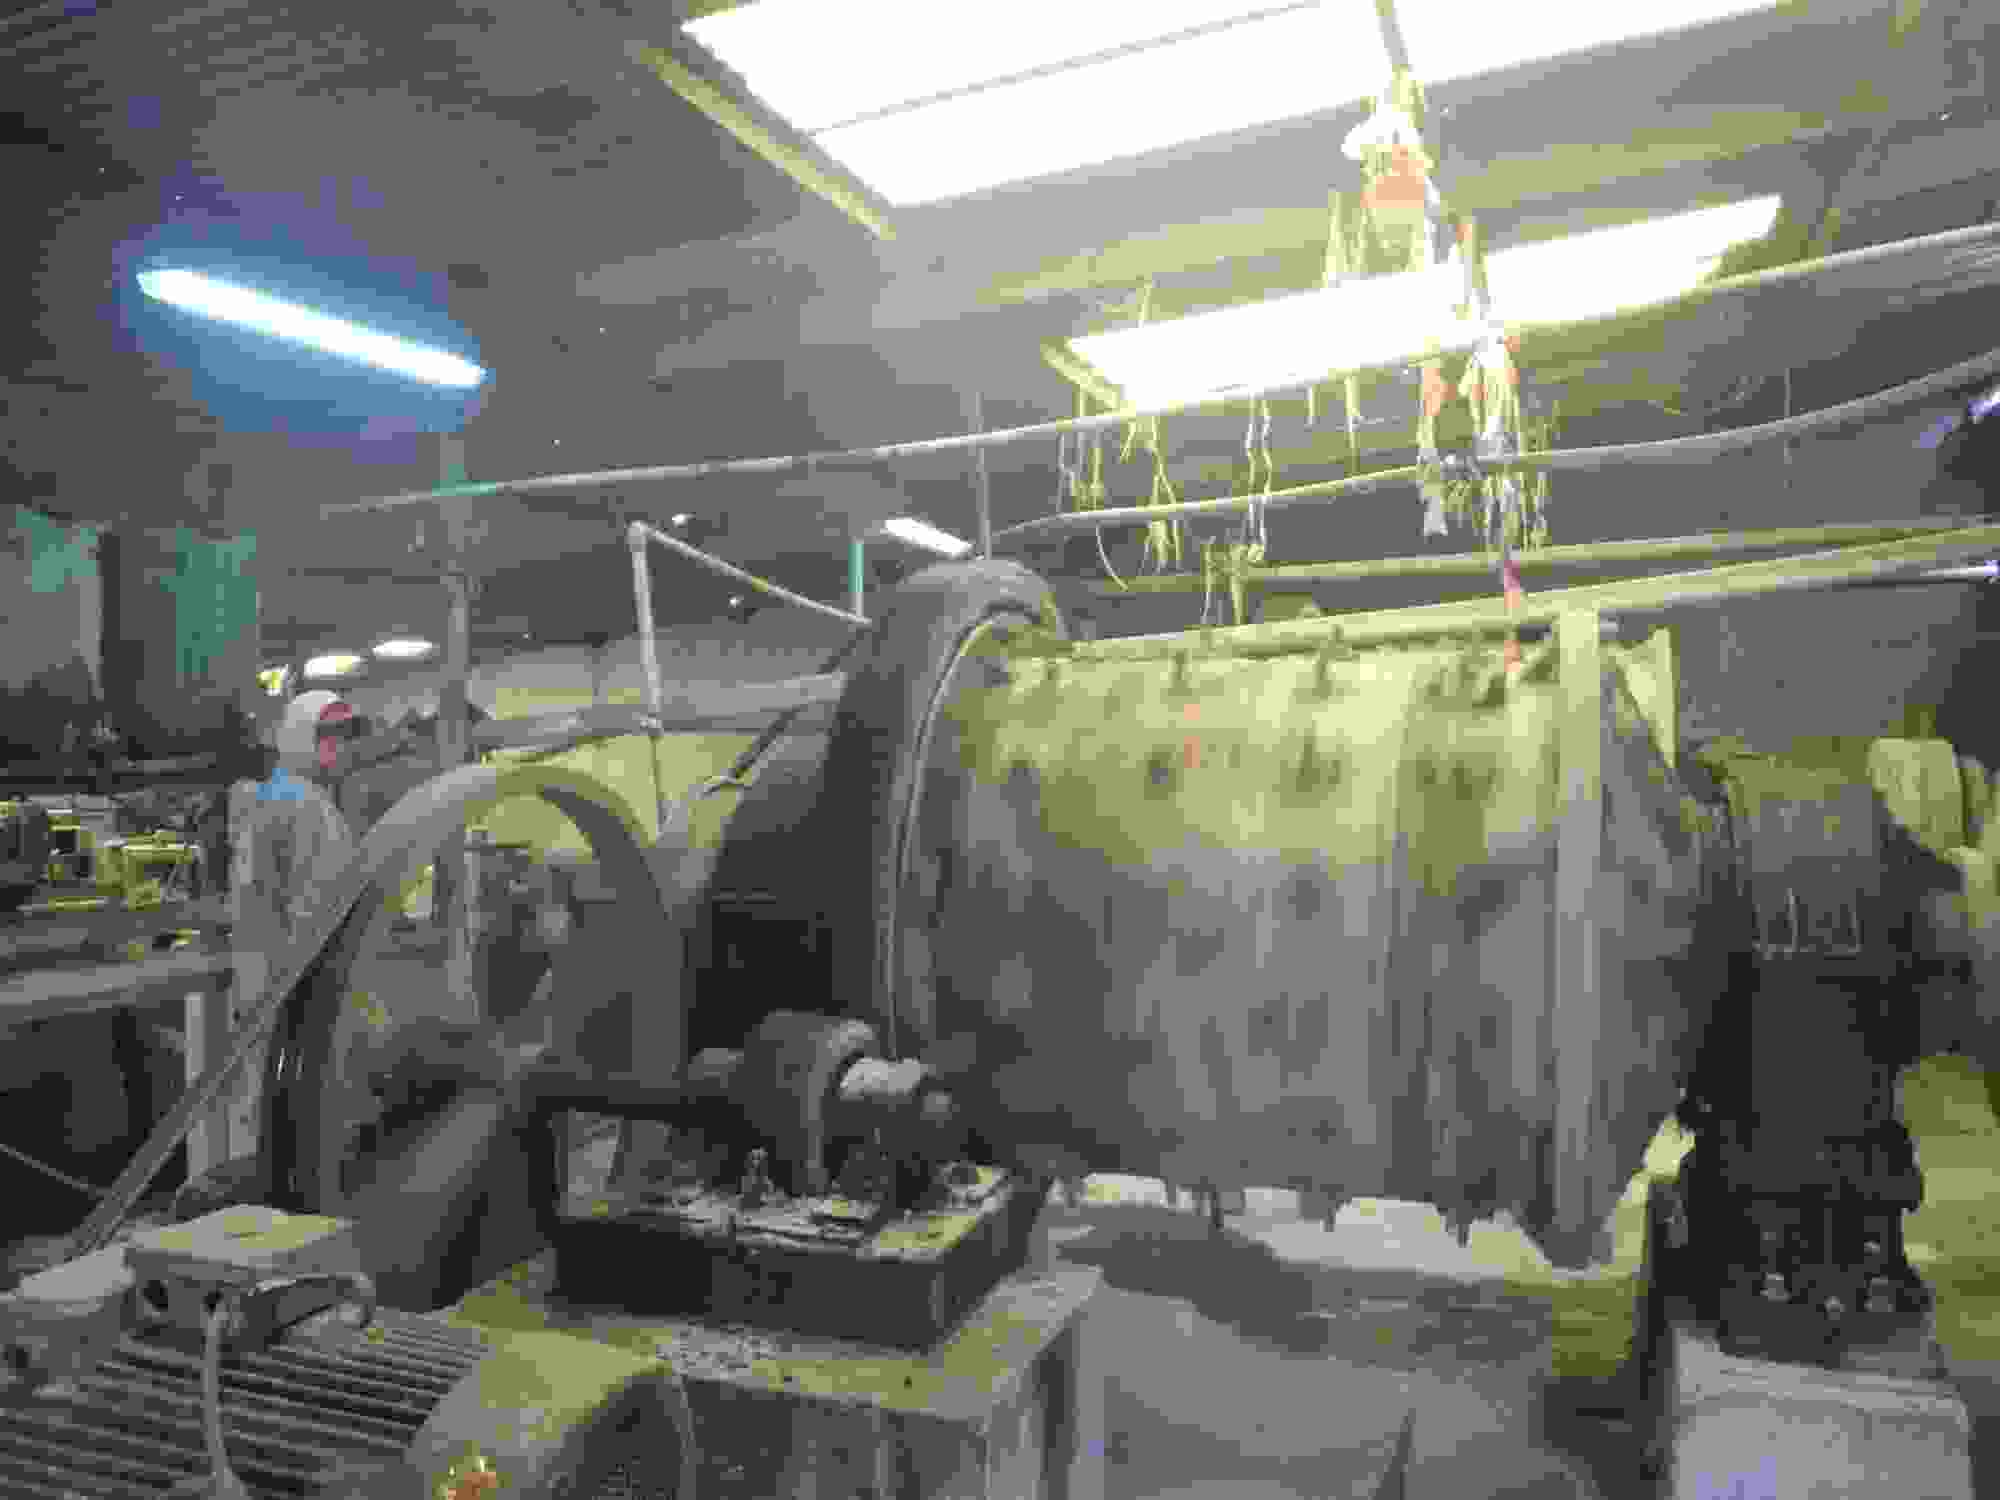
\includegraphics[width=\mywidth]{../wp-content/uploads/2015/04/wpid-wp-1428892501544.jpg} \end{center}
\begin{center} 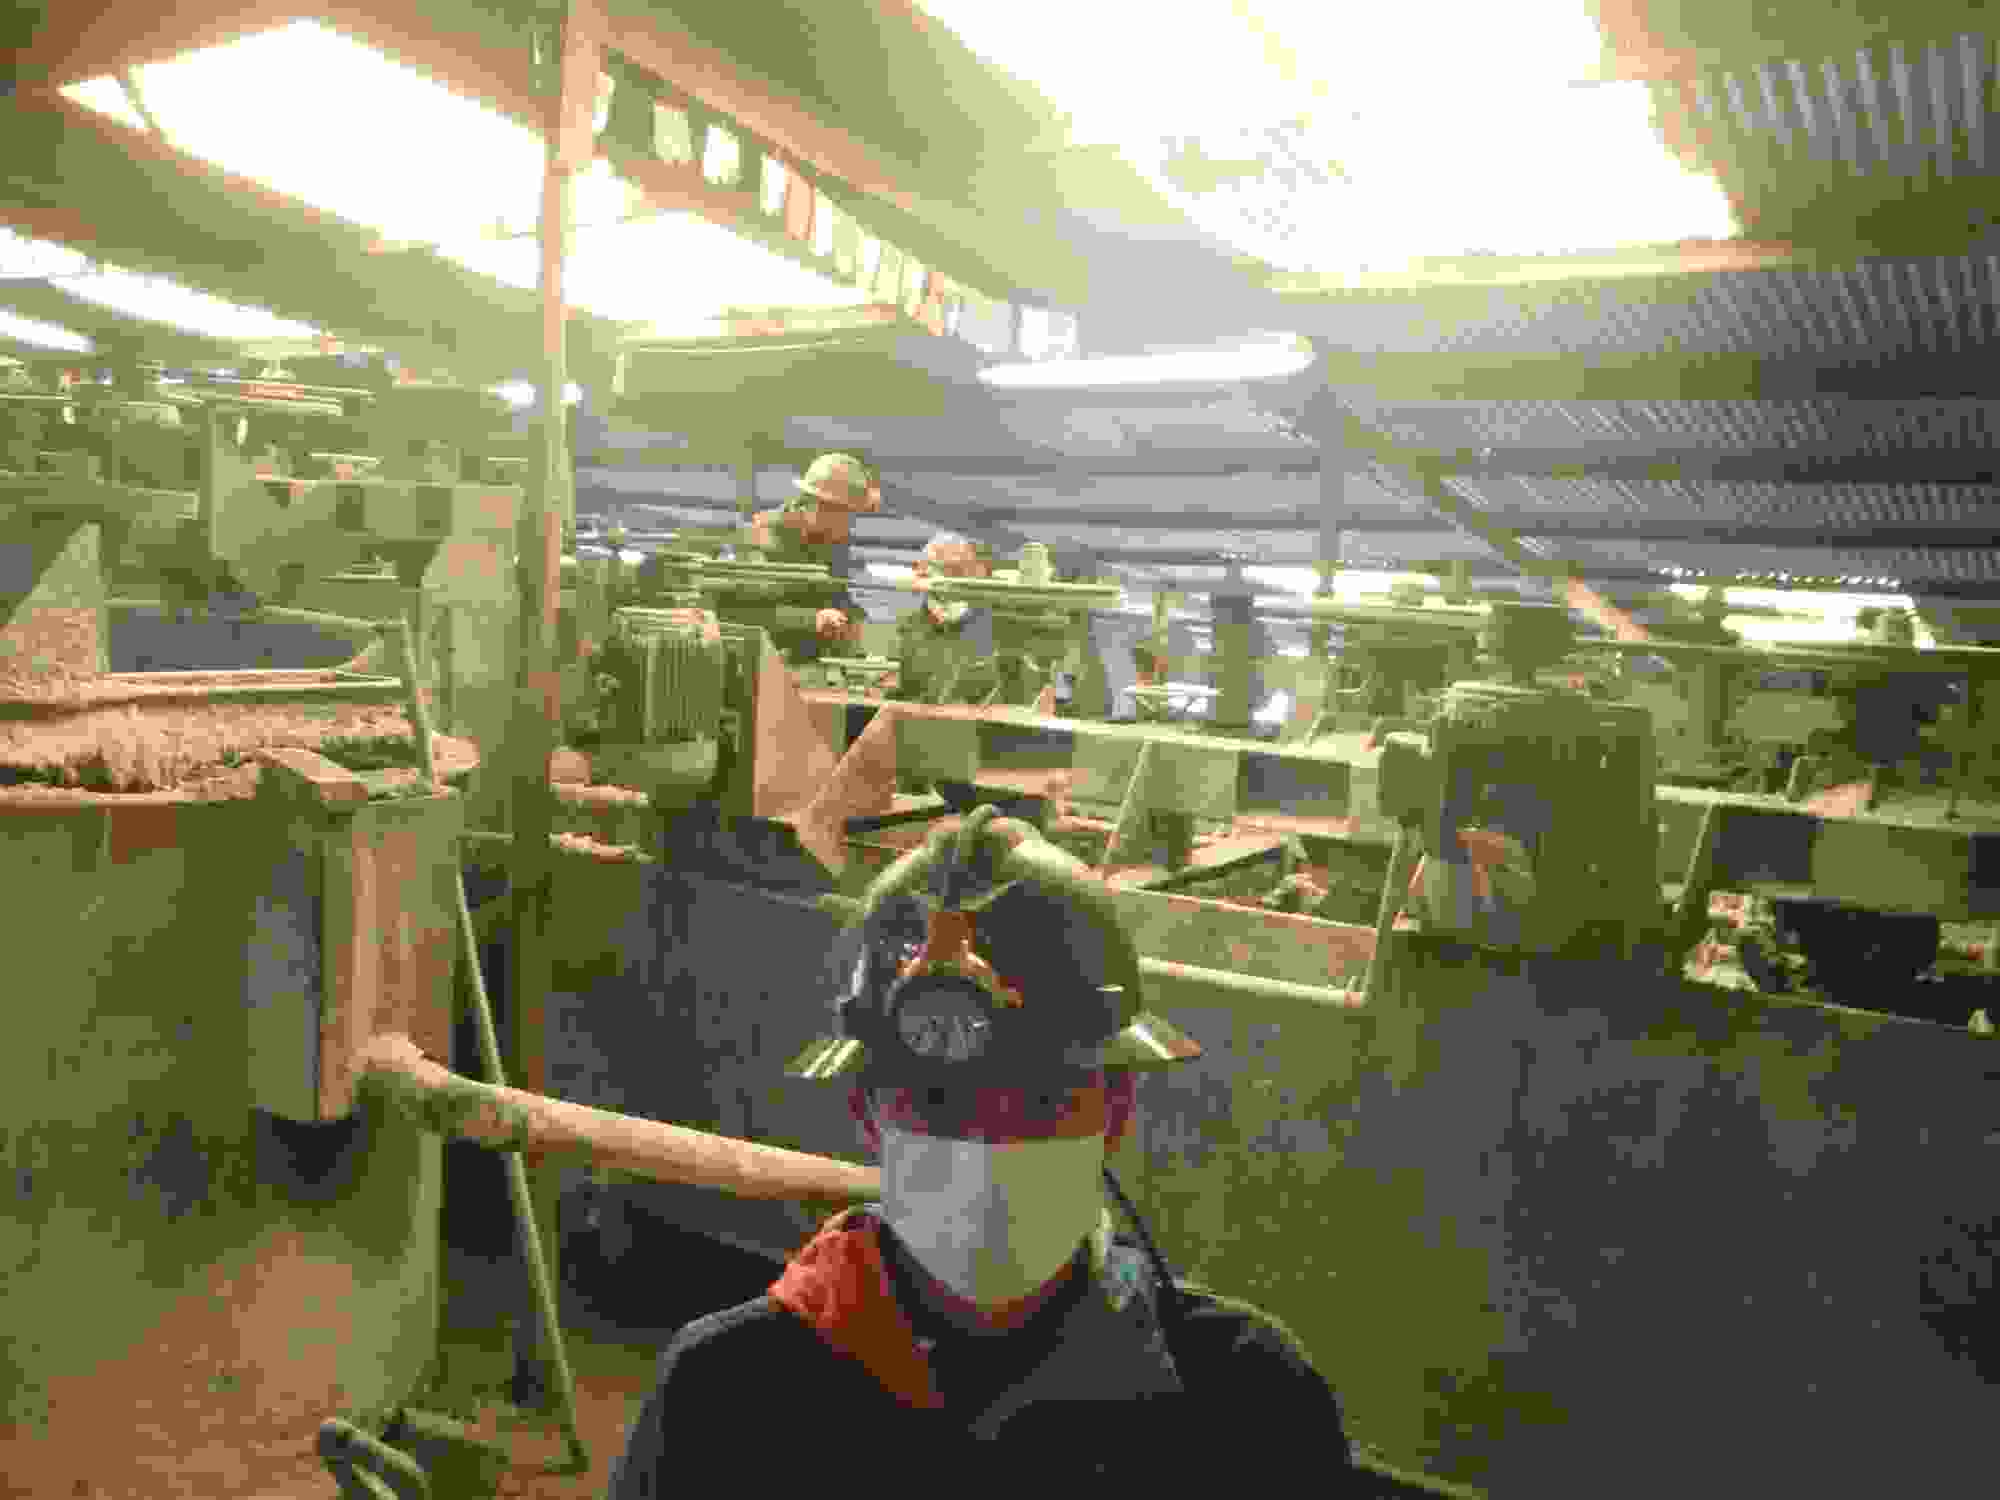
\includegraphics[width=\mywidth]{../wp-content/uploads/2015/04/wpid-wp-1428892515847.jpg} \end{center}

 Puis c'est la visite de la mine, guidée par un ancien mineur. 
\begin{center} 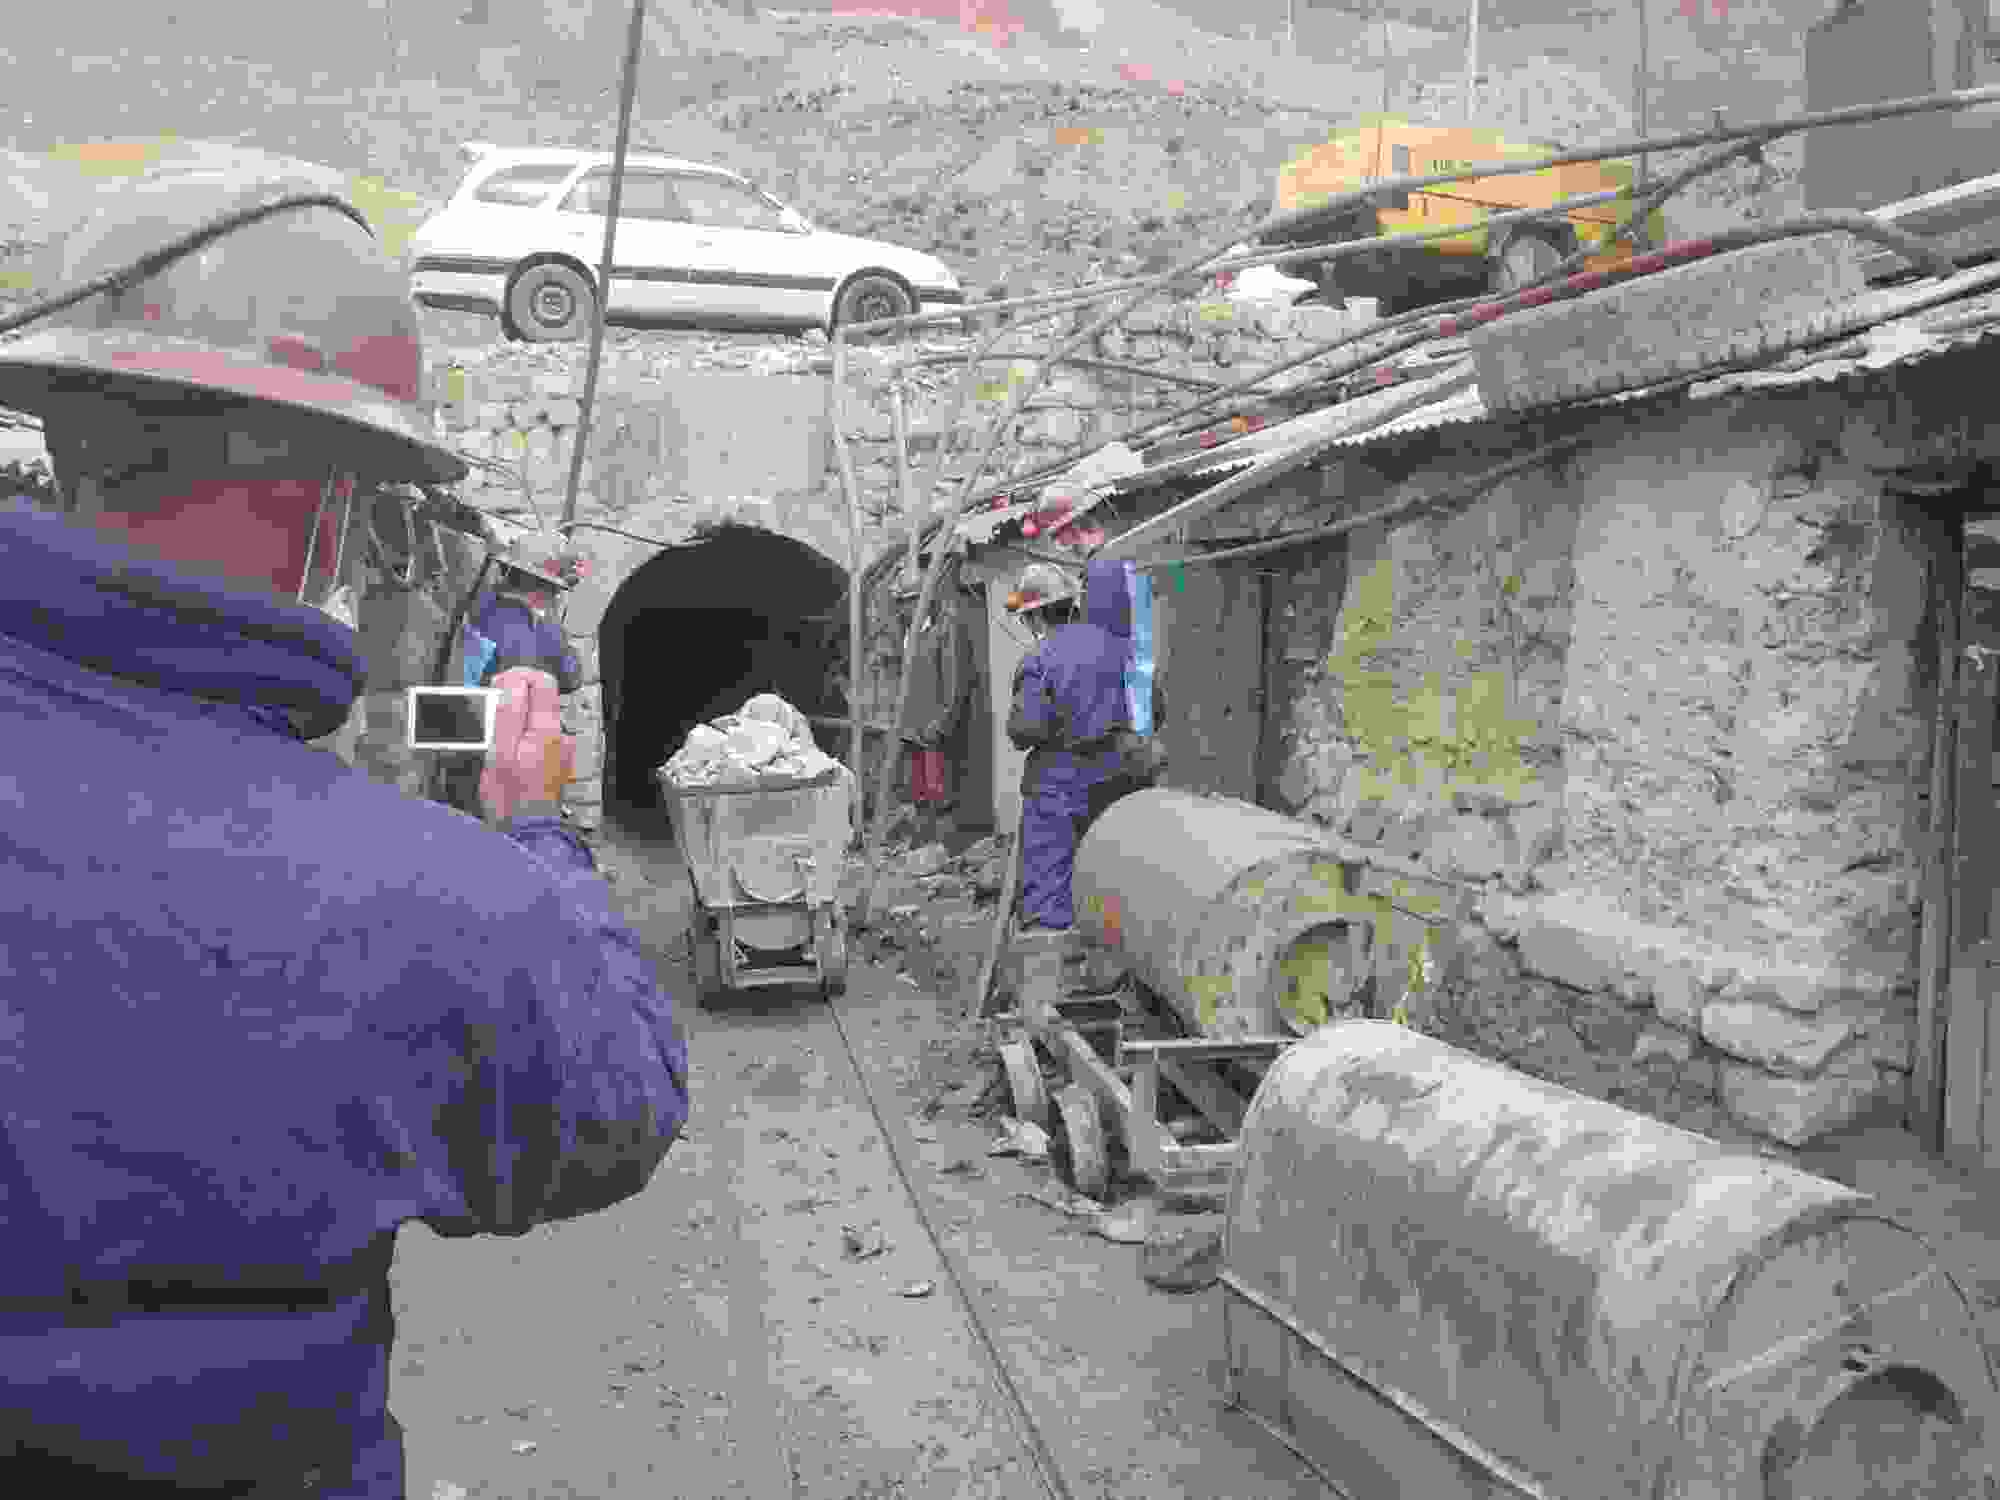
\includegraphics[width=\mywidth]{../wp-content/uploads/2015/04/wpid-wp-1428892613443.jpg} \end{center}
\vspace{-\topsep}

\pagebreak
 \og El Tio \fg\ porte bonheur pour les mineurs. 
\begin{center} 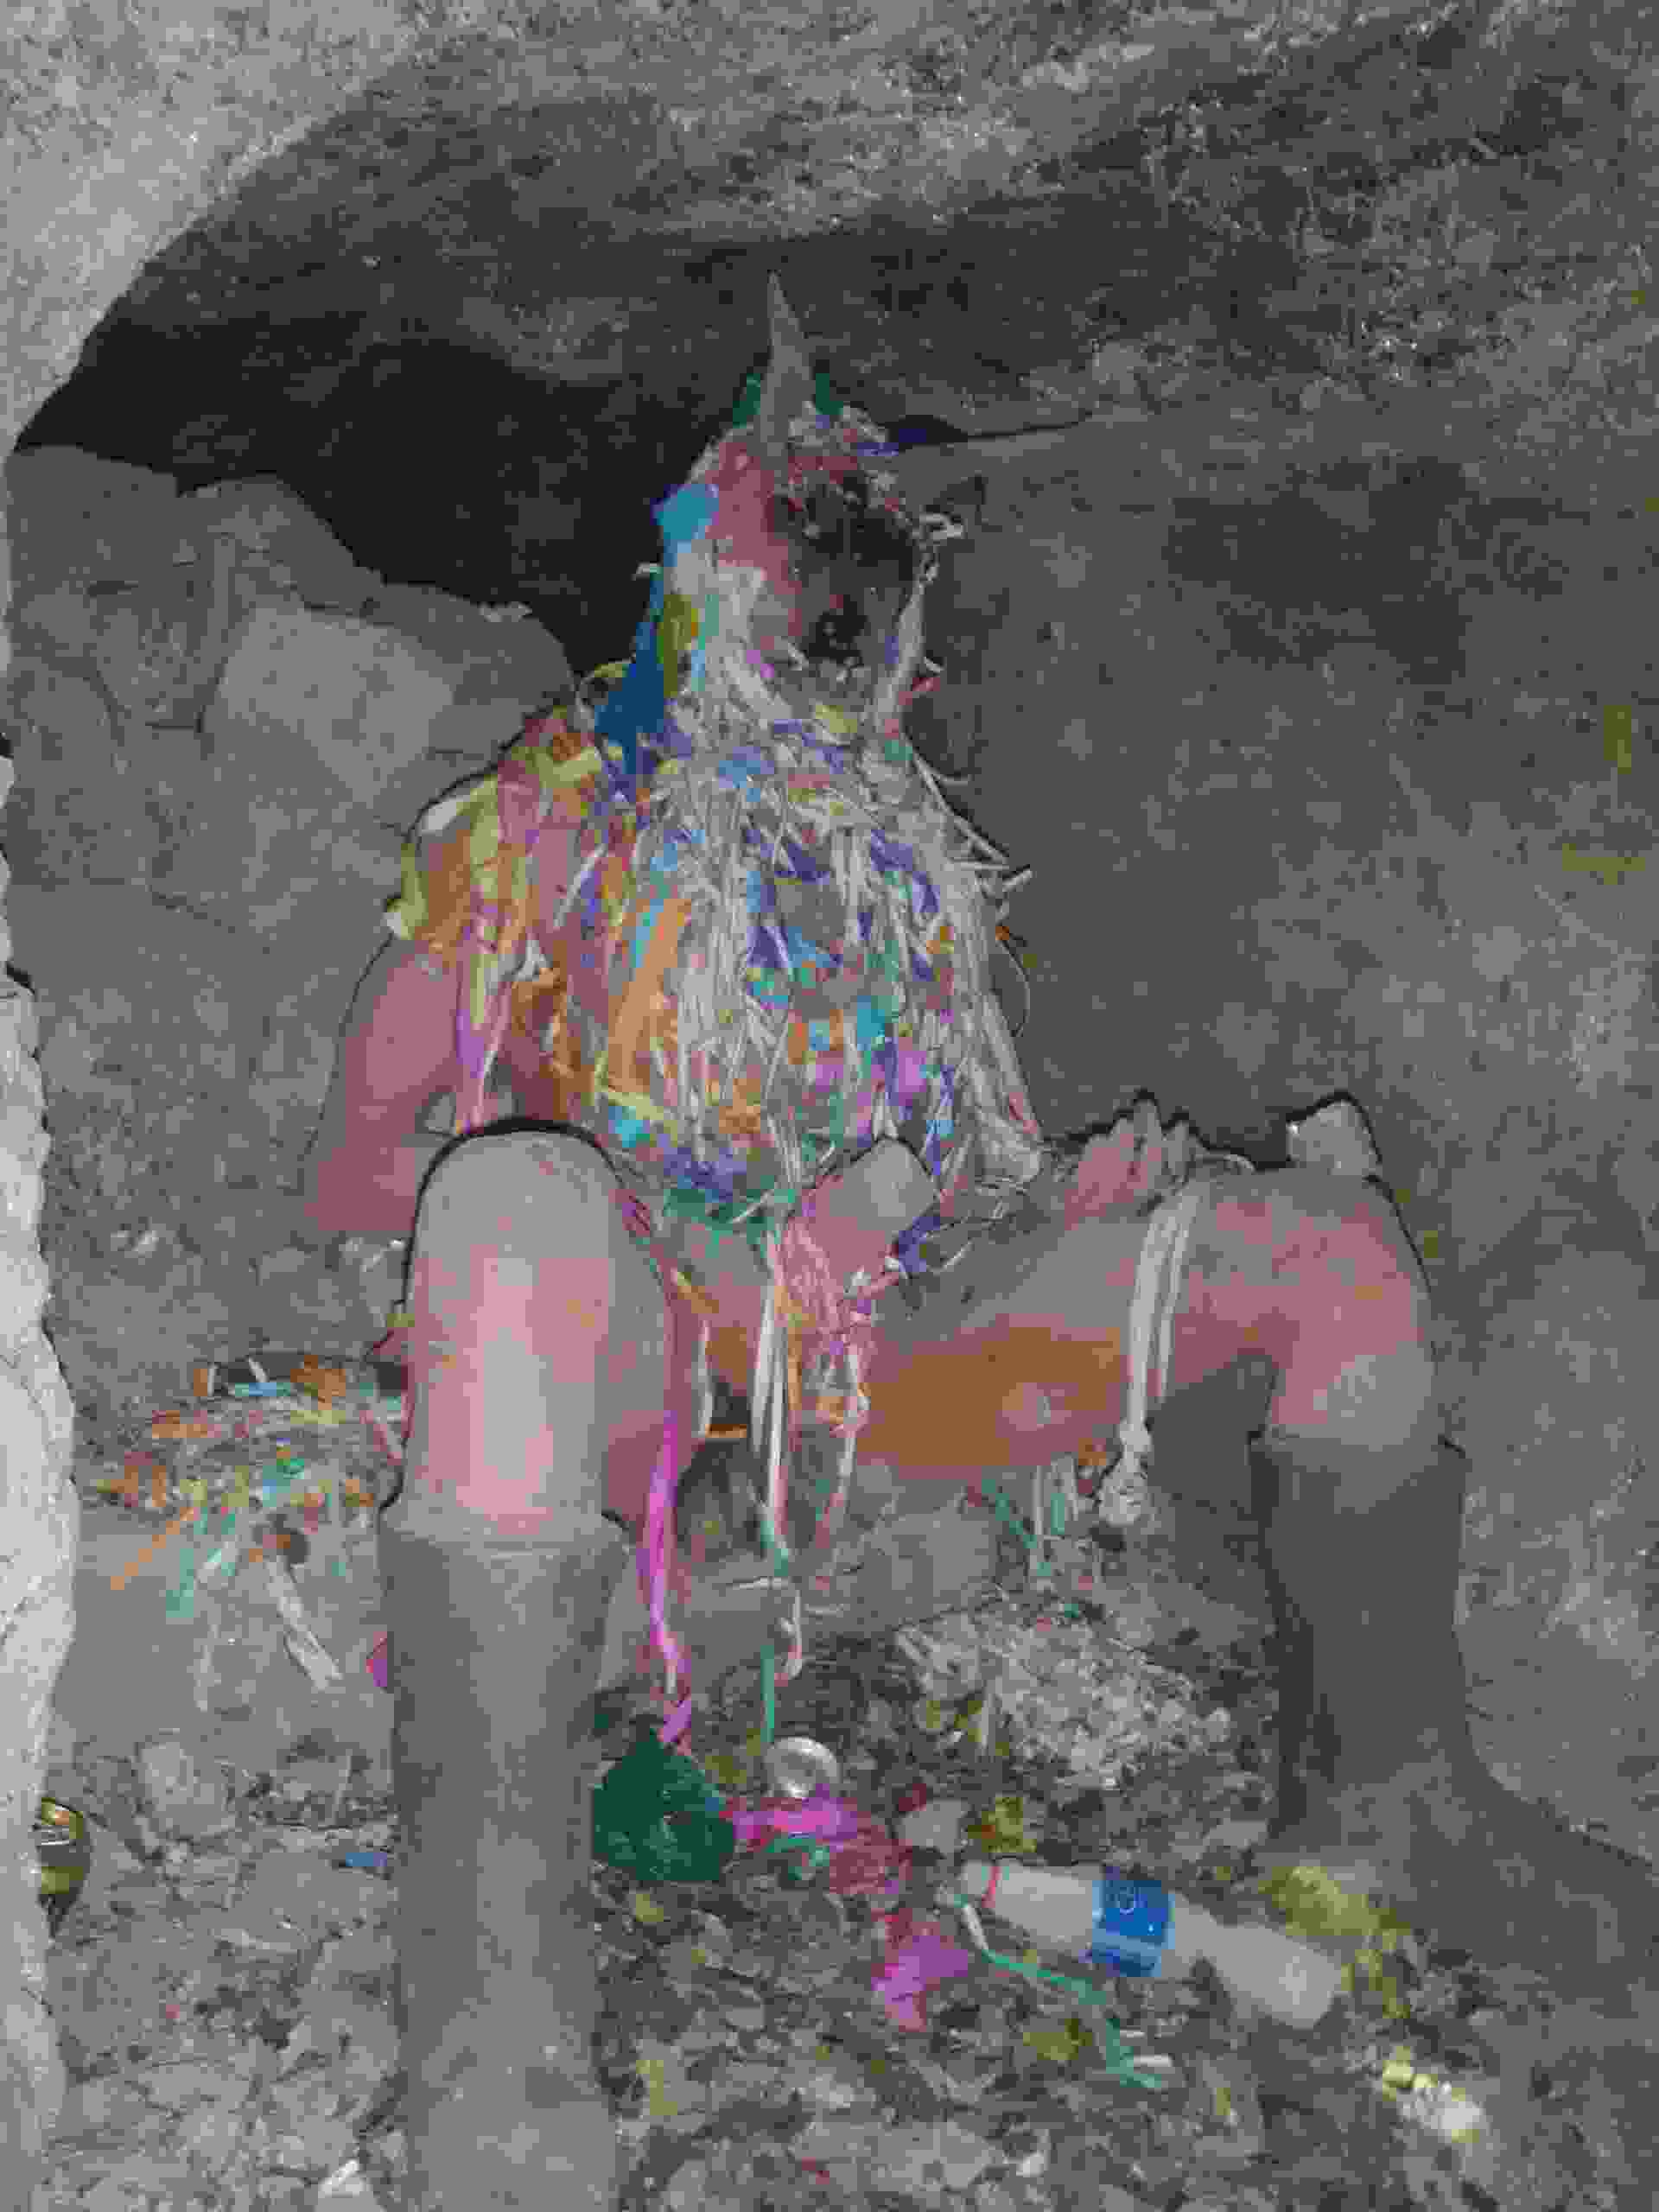
\includegraphics[height=0.79\textwidth]{../wp-content/uploads/2015/04/wpid-wp-1428892725739.jpg} \end{center}

Les galeries, on doit marcher courbé et la plupart du temps dans la boue. 
\begin{center} 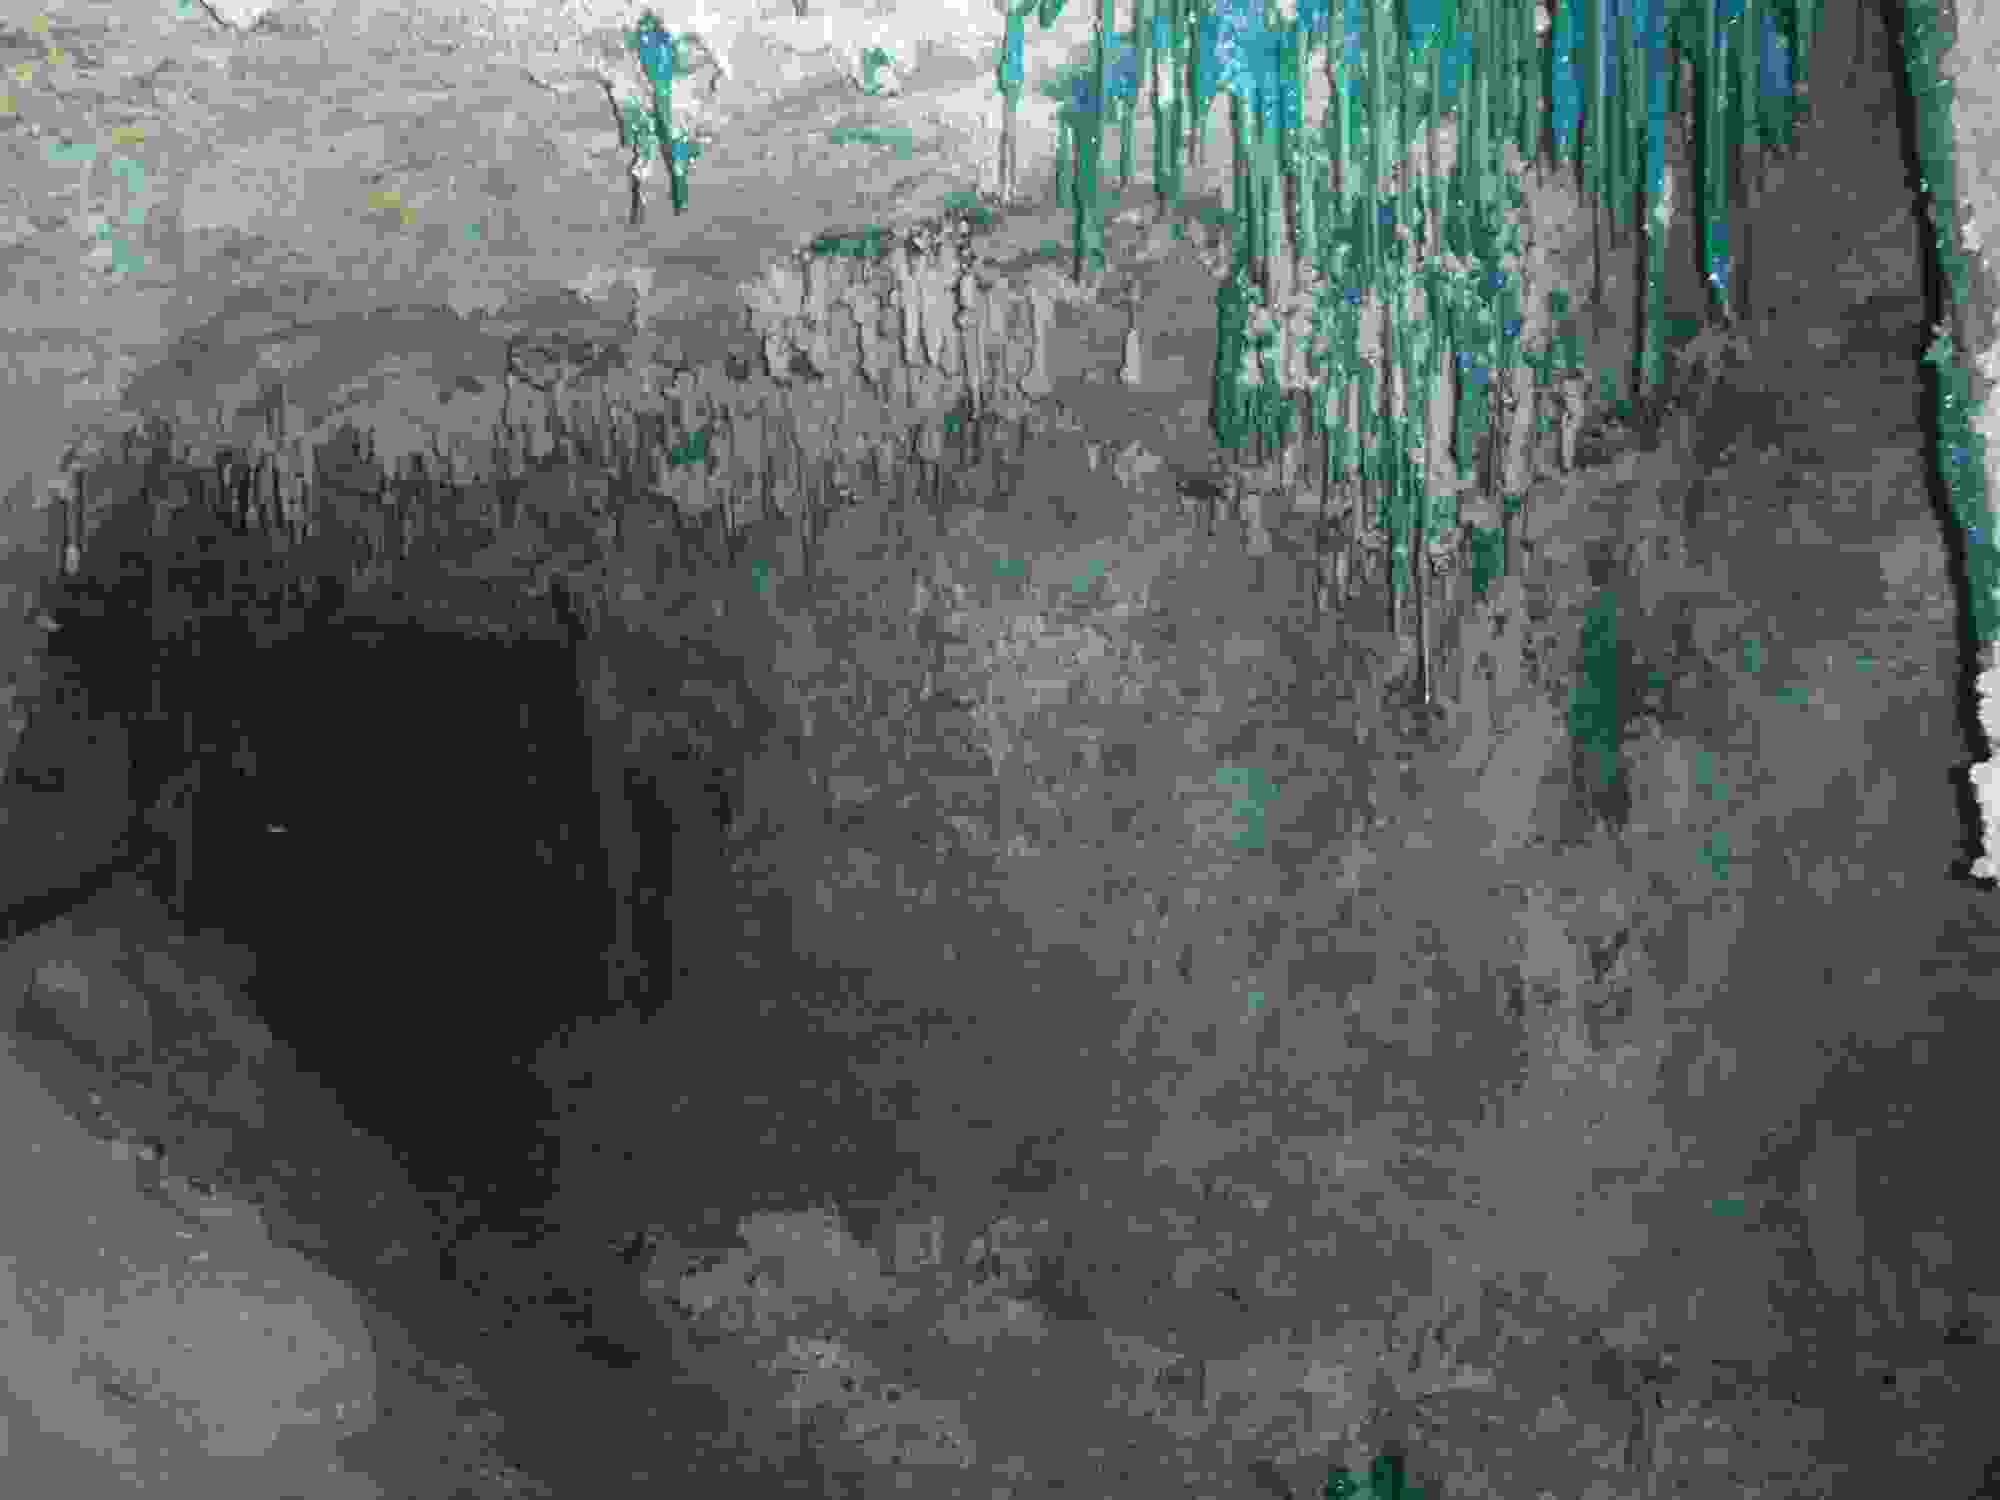
\includegraphics[width=\mywidth]{../wp-content/uploads/2015/04/wpid-wp-1428892808307.jpg} \end{center}

 On croise quelques mineurs : les feuilles de coca leur donnent l'énergie pour travailler toute la journée sans manger. 
\vfill
 Ce travail usant et dangereux leur permet de gagner 2 à 3 fois le salaire minimum bolivien. 
 \vfill
\begin{center} 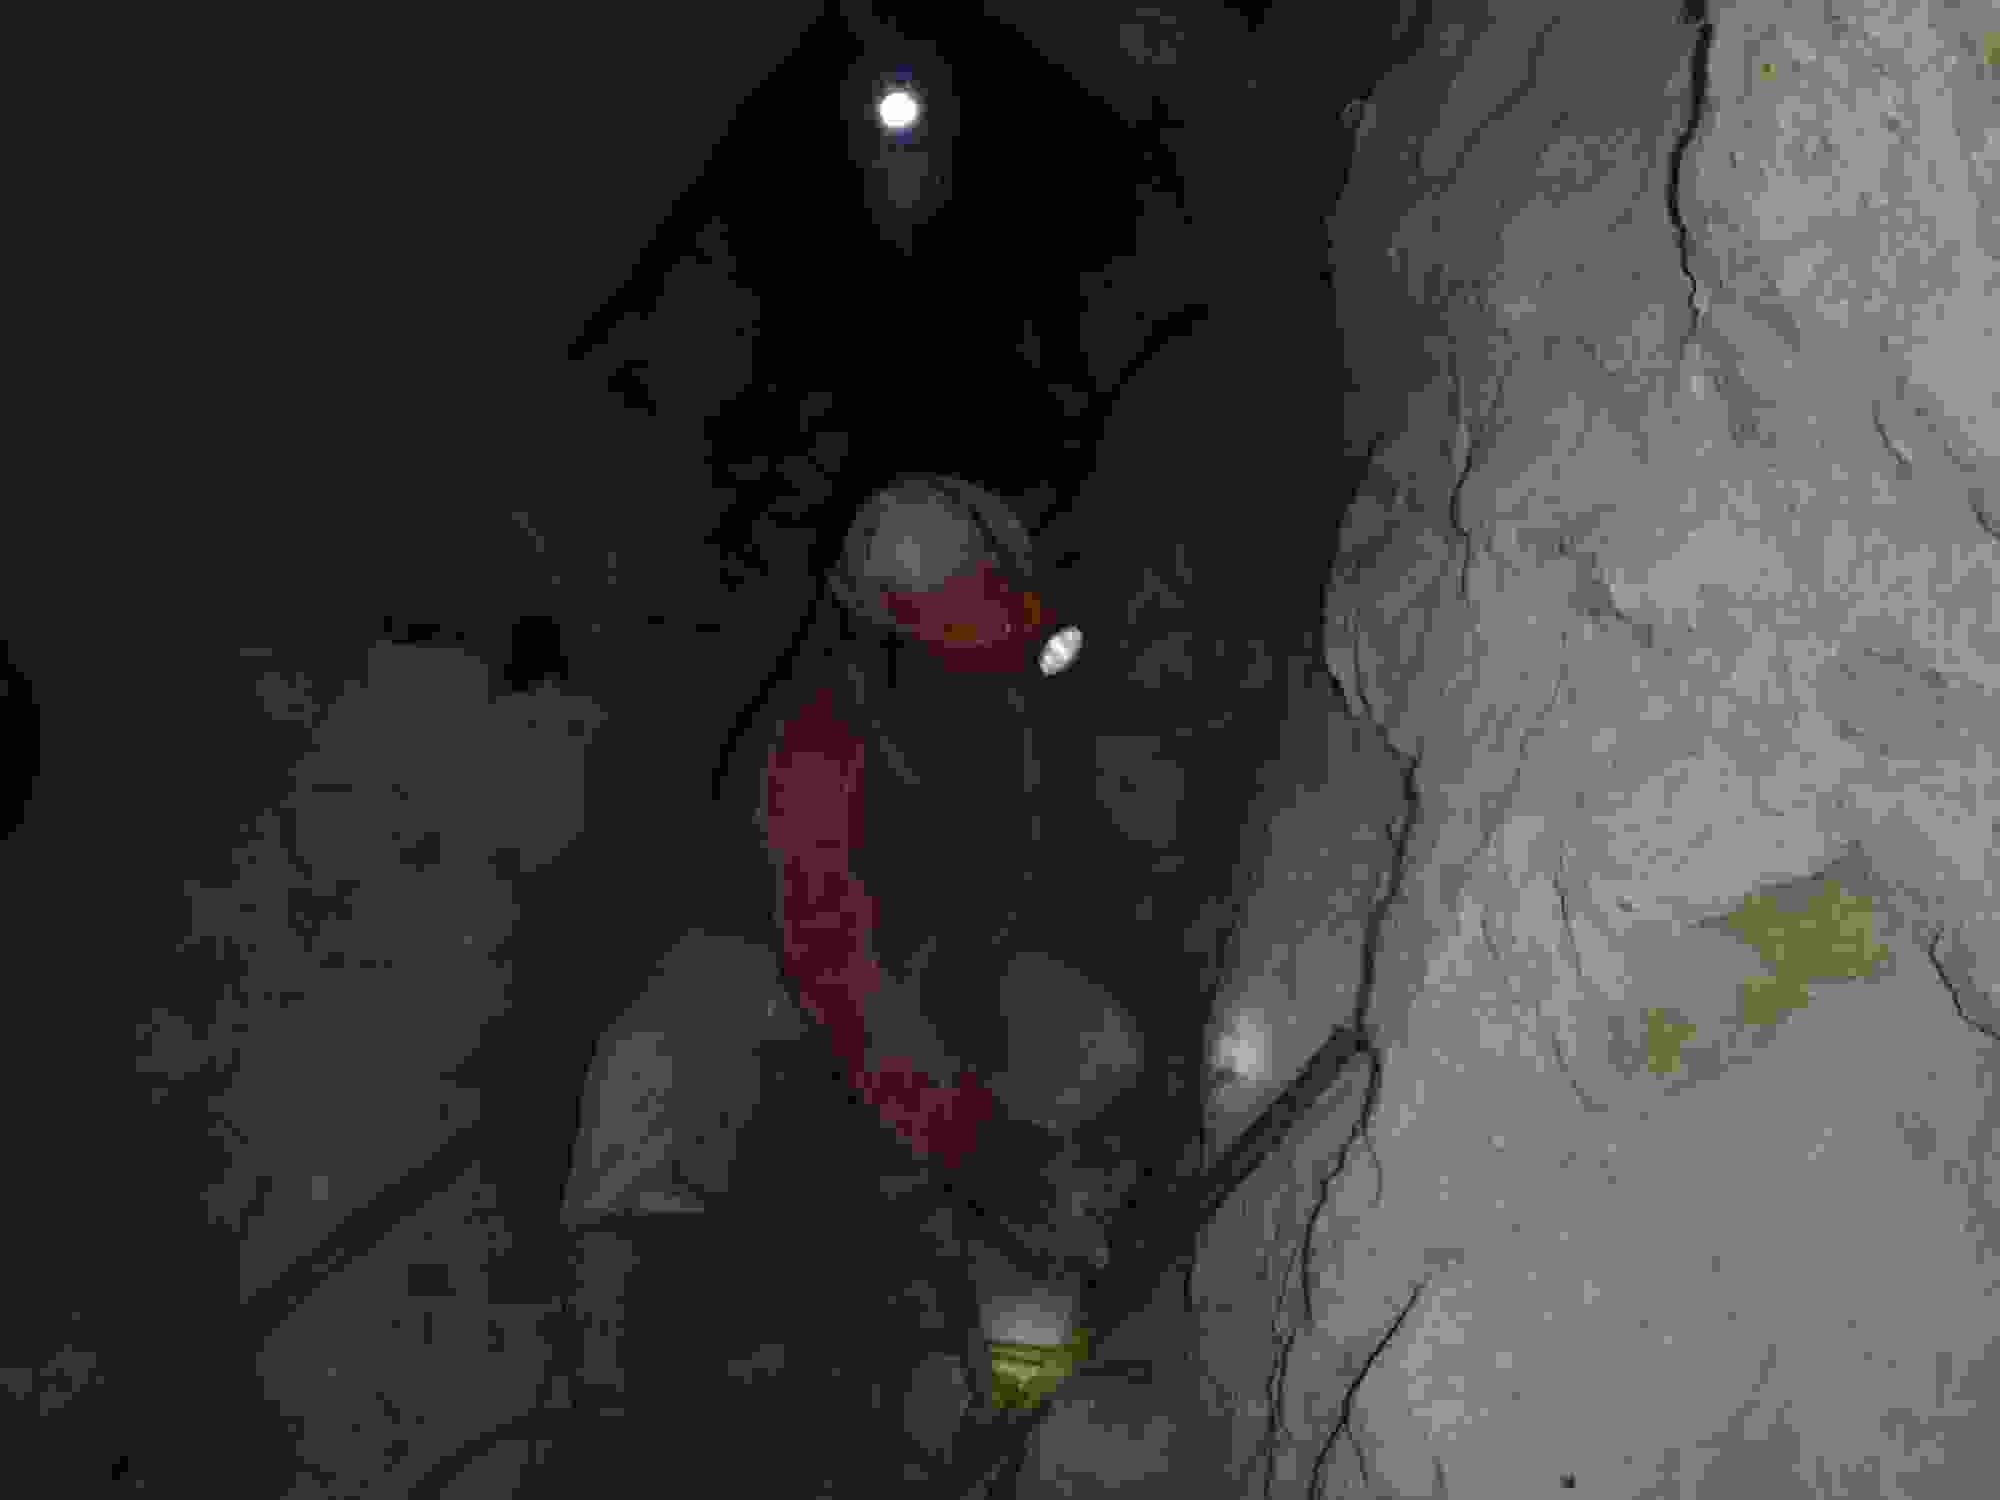
\includegraphics[width=\mywidth]{../wp-content/uploads/2015/04/wpid-wp-1428892913145.jpg} \end{center}
\vfill
\begin{center} 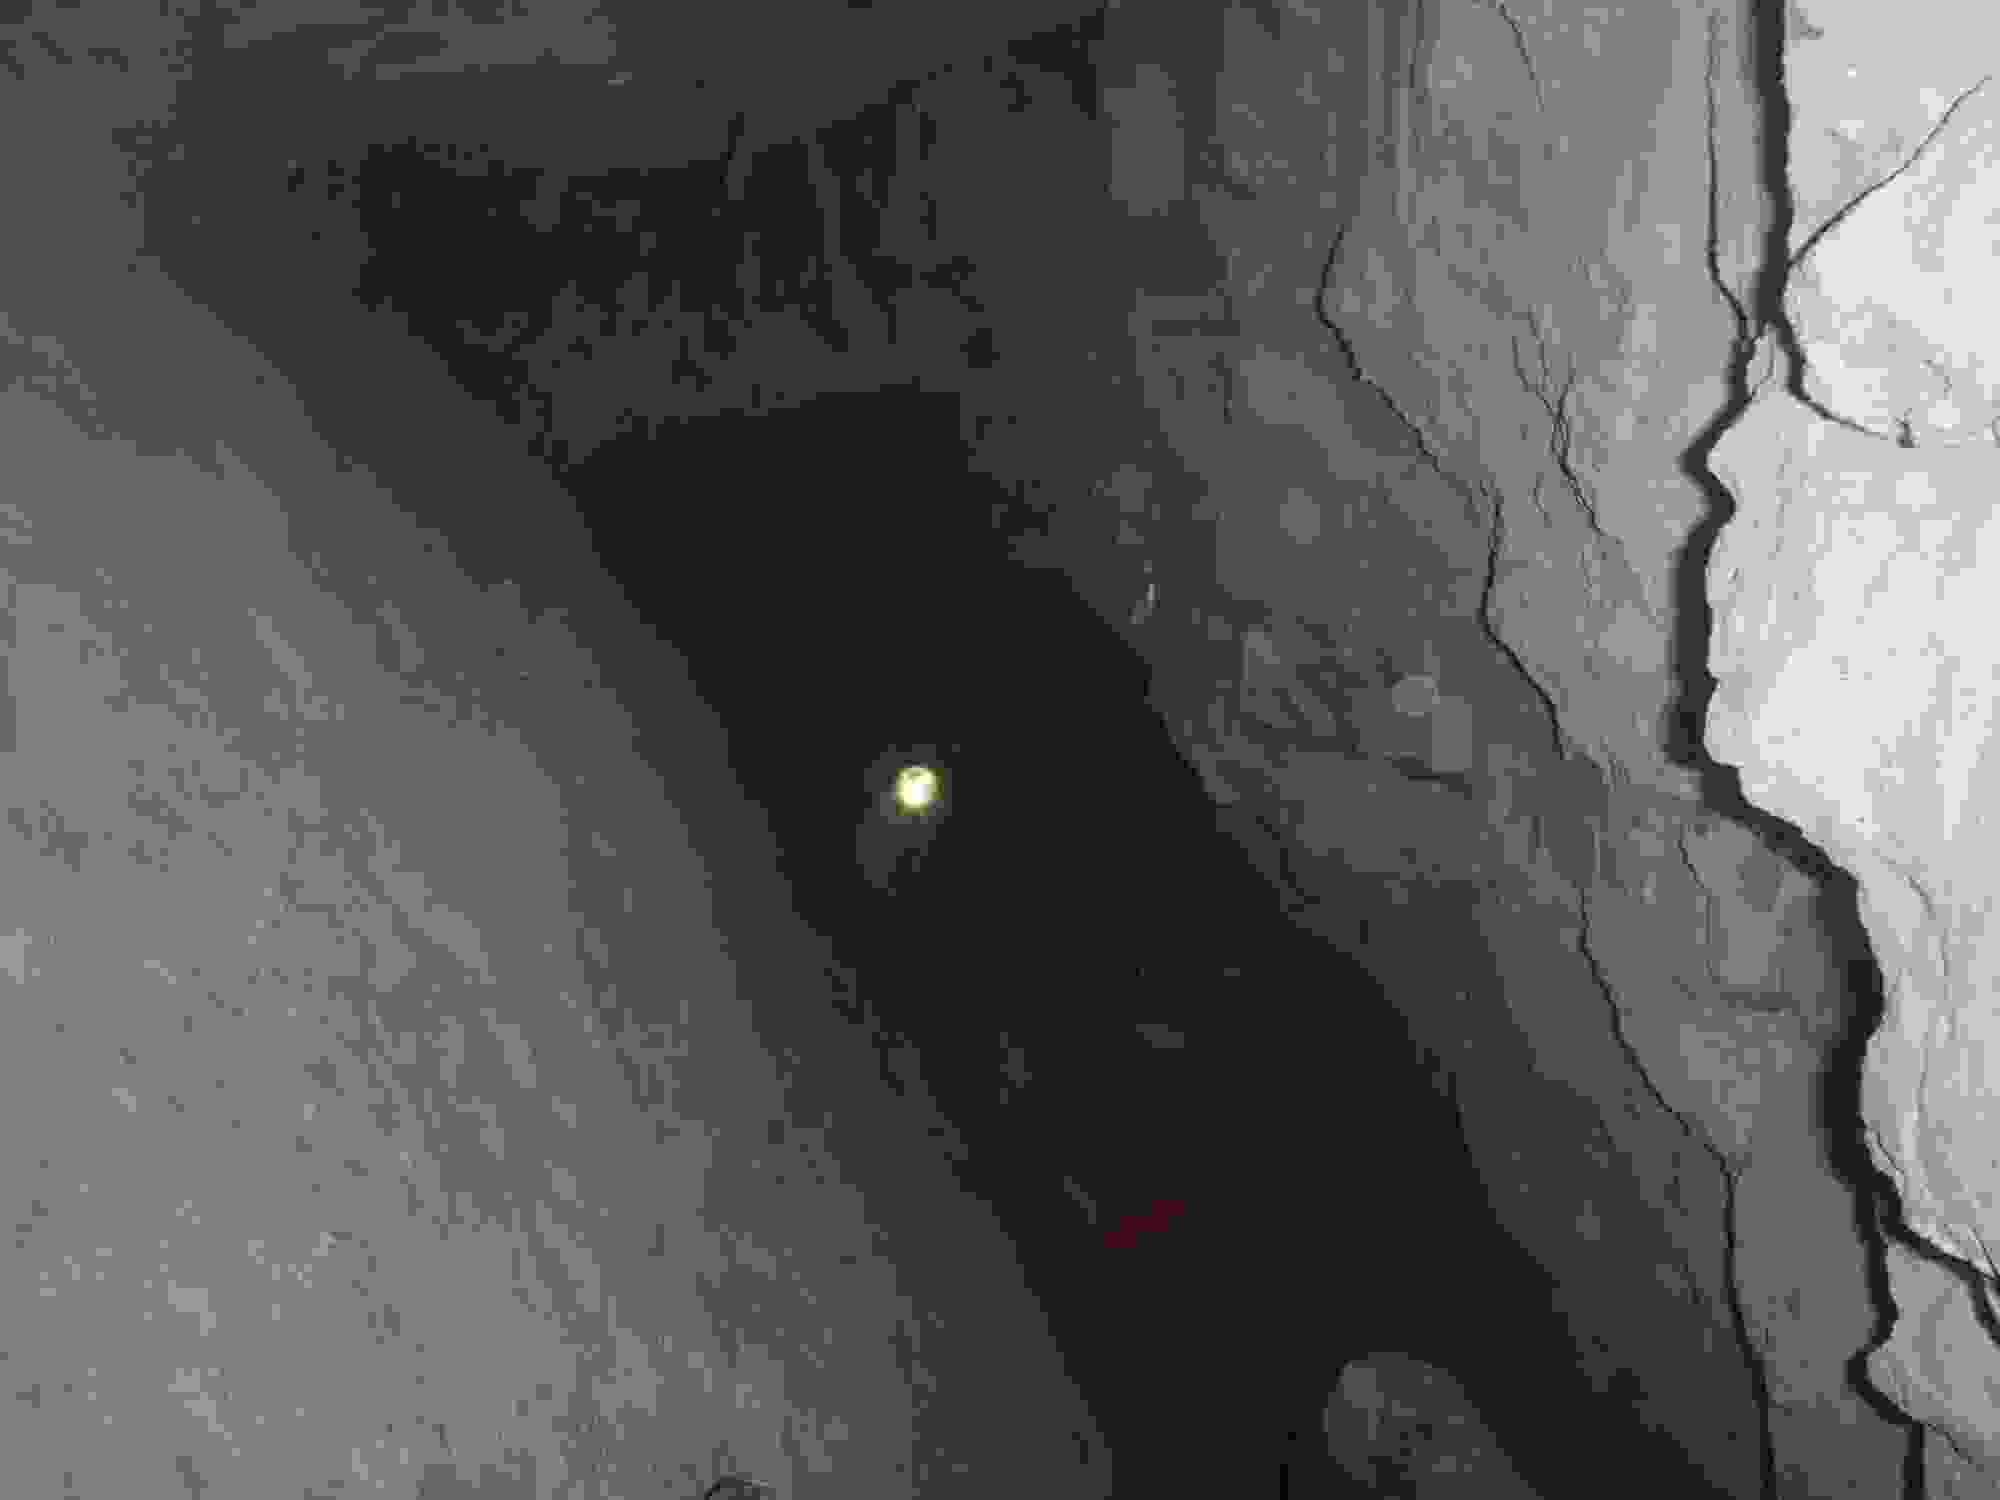
\includegraphics[width=\mywidth]{../wp-content/uploads/2015/04/wpid-wp-1428892926957.jpg} \end{center}
\vspace{-\topsep}
\vspace{-0.75mm}